\documentclass[a4paper,11pt,titlepage]{article}
\usepackage[margin=2cm]{geometry}

\usepackage[nodayofweek]{datetime}
\longdate

\usepackage{fancyhdr}
\pagestyle{fancyplain}
\fancyhf{}
\lhead{\fancyplain{}{M.Sc.\ Individual Project Literature Survey}}
\rhead{\fancyplain{}{\today}}
\cfoot{\fancyplain{}{\thepage}}
\usepackage{adjustbox}

\usepackage[english]{babel}
\usepackage[utf8x]{inputenc}
\usepackage{float}

\usepackage{amsmath}
\usepackage{graphicx}
\usepackage{cite}
\usepackage{hyperref}
\usepackage{caption}
\usepackage{subcaption}



\title{Browser-based Medical Image Viewer using WebGL \\\Large{--- Report ---}}
\author{David Basalla\\
  \small{Supervisor: Dr.\ Ben Glocker}\\
  \small{Imperial College London}
}

\begin{document}


\begin{titlepage}

\newcommand{\HRule}{\rule{\linewidth}{0.5mm}} % Defines a new command for the horizontal lines, change thickness here

\center % Center everything on the page
 
%----------------------------------------------------------------------------------------
%	HEADING SECTIONS
%----------------------------------------------------------------------------------------

\textsc{Imperial College London}\\[0.5cm] % Minor heading such as course title
\textsc{Department of Computing}\\[8.5cm] % Minor heading such as course title


%----------------------------------------------------------------------------------------
%	TITLE SECTION
%----------------------------------------------------------------------------------------


{ \large \bfseries Browser-based Medical Image Viewer\\* using WebGL}\\[0.4cm] % Title of your document
{ \large \bfseries by}\\[0.4cm] % Title of your document
{ \large \bfseries David Basalla}\\[10cm] % Title of your document
 


%----------------------------------------------------------------------------------------
%	DATE SECTION
%----------------------------------------------------------------------------------------

{Submitted in partial fulfilment of the requirements for the MSc Degree in Computing Science of Imperial College London }\\[0.5cm] 
{September,  2014}\\[0.5cm] % Minor heading such as course title



\vfill % Fill the rest of the page with whitespace

\end{titlepage}



\tableofcontents


\newpage
\section{Introduction}

Medical imaging is a type of scientific visualisation that deals with analysis, representation and exploration of medical image data. It should aid in diagnosis, treatment planning, support in actual operations, documentation and educational purposes. Medical imaging is primarily based on 3D volume data acquired by scanning devices such as computed tomography and magnetic resonance imaging. The resulting data files are viewed with specific computer software and contain a wealth of data. This software traditionally needs to be installed on a local computer machine. With the rise of WebGL, a powerful 3D Graphics API for the Web that makes use of the local graphics card, this project will investigate the general plausability and specific implementation of a Web Browser based medical image viewer. This should free the user from having to use desktop bound software and instead enable him to simply log on to a website in his prefered Web Browser.

\subsection{Motivations}

To view medical image data, users are required to have appropriate software installed on their local desktop computer. This involves a varying download or installation process. Additionally software developers have to cater for different operating systems when writing these programs. To overcome these issues, the goal of this project is to provide a medical image viewer that runs in any Web Browser. This web-app will aim to provide the functionality as a desktop solution without being tied to a specific operating system. It furthermore aims to provide an intuitive and complete set of tools for viewing multiple files and allowing for creation, viewing and manipulation of label maps and other methods of annotating these images. The rationale behind this is to facilitate users to conveniently view, edit and annotate medical image files independently of location or type of computer, following the "Software as a Service" paradigm.


\subsection{Requirements}


The goal of this project is to build a Web Browser based Medical Image Viewer. This will be achieved by making use of \textit{WebGL} to display 2D and 3D graphics. In general the project aims to provide similar functionality and user experience as the desktop application \textit{MITK} (discussed earlier). The essential requirements are as follows:

\begin{itemize}
\item The user can load and view a scan file (of type \textit{NIfTI})
\item The user can view a file in 2D and 3D
\item The user can easily navigate through the 2D and 3D viewers, with emphasis on intuitive user experience
\item The web-app provides controls for viewing the scan files at different brightness and contrast levels
\item The user can load and view a labelmap for a given scan file
\item The user can load additional scan or label maps into the viewer and compare them to previously loaded files with a set of intuitive controls
\item Provide different color-lookups (for label-maps, heat maps)
\item Provide sample data to use if user has no files of his own
\end{itemize}

Given enough time, secondary requirements can be implemented, which are considered to be more complicated:

\begin{itemize}
\item The user can paint a custom labelmap for a given scan file with a set of intuitive tools. The primary goal will be that the user can paint areas manually on individual slices. Provided there is enough time, some semi-automatic painting tools will also be implemented that will allow the user to specify regions in the 3D space with automatic selection tools. 
\item The user can save a labelmap to his computer
\item The user can create and save custom annotation maps to label given scans
\item The web app provides a method for sharing  means of sharing data across the internet (similar to the DropBox implementation in SliceDrop)
\item The web app provides image filters that can be applied to a scan or label map
\item The web app provides measuring tools that can be applied to a scan or label map
\item A three dimensional, parameterised model of the scan be viewed in the 3D view
\item The 'cine mode' feature allows for an animation along a specified axis
\end{itemize}


\subsection{Use Cases}

A small selection of use cases have been discussed with the project supervisor. The following were suggested:

\begin{itemize}

\item A user loads two medical images files from a patient that has undergone brain surgery. The user wants to compare the scans from before the operation to afterwards. The user needs to be able to compare the two files in meaningful ways, with tools for image comparison and compositing.

\item A user wants to create a custom label map by highlighting a certain section of a loaded scan. The user can use provided paint tools to paint individually on each slice, or alternatively use semi-automatic tools like filling in regions within a given color range to speed up this process. The user can save out this custom label map in \textit{NIfTI} format.

\item The user wants to create annotations for a file. He can use the software to create annotated planar or cuboid regions to for example specify where a given organ is in the scan. The software provides intuitive controls and helpful visual feedback to facilitate this process. The user can save out this files as a custom data file.

\item A user wants to communicate with another user who is not present in the same location. The first user can use the software to provide links to specified medical image files to the second user. The second user can load these files with the software for analysis.

\end{itemize}







\subsection{Contributions}

The final software represents a comprehensive tool for viewing medical image data as well as adding custom annotations . All of the primary aims as stated above have been met, as well as a couple of secondary requirements (see full feature list in the Implementation Section). It is designed to be used with intuitive control as advised for use by radiologists, mimicking convential controls in other software. Judging by similar software online, the software provides many more features than its competition. It has also been tested to successfully run across several operating systems and Web Browsers, thereby fulfilling the requirement of being more widely useable independent of computer configuration of the user. The project was built on using the XTK library, which appears to be the most comprehensive library for viewing medical image data to date. However since missing a lot of critical functionality as required by this project, the library had to be extended to provide tools for more dynamic application building.

\newpage
\section{Background}



\subsection{Medical Imaging}



As mentioned, medical image files are acquired by scanning devices such as CT, MRI or PET scanners that output data at a given resolution of data points. A typical medical image file contains a stack of individual images. Each image represents a thin slice of the scanned body part and is made up of pixels. For a volume data set the stack of images can be usually subdivided into cross sections along the three Cartesian axes X, Y and Z and together form a 3D Grid. In medical terms, these orthogonal views are called axial, sagittal and coronal. A constant pixel distance along X and Y allows for accurate measuring of distances and areas along a slice. The slice distance is the measurement in space from one slice to the next along its cross section. The three distances in every direction is called the voxel distance. If the pixel distance is equal to the voxel distance, the dataset is called isotropic. However in practice datasets usually exhibit a much smaller pixel distance than slice distance, which is called anisotropic.
Measuring cross-sectional areas and volumes are valuable for example in diagnosis of vascular diseases. The quality of these measurements is highly dependent on the quality of the image data. Typically diagnosis has been performed these slices one at a time, meaning looking at every slice. These views support precise exploration and analysis and it is a legal requirement for radiologists to inspect every slice. However for spatially complex cases a purely slice-based presentation might not be very helpful. In this case 3D visualisation or volume rendering gives a better overview. The two different visualisations can be helpful for different users, such that radiologists would rely more on the 2D Views and physicians who carry out interventions might find benefit from 3D visualisations. Therefore any software that aims to display such medical image data should provide both views.


\begin{figure}[ht!]
\centering
\includegraphics[width=90mm]{..//literatureSurvey/graphics/book_2d3d_01.jpg}
\caption{2D View (left) and 3D View (right) - REFERENCE}
\label{fig:UIdesign1}
\end{figure}



\subsection{Guidelines for Medical Image Viewer Software}

As defined in 'Visual Computing in Medicine'\cite{book}, a program needs to provide the following functionality in order to be of use when displaying this kind of medical imaging data. 

First, a certain mapping of data to gray values has to occur, called 'windowing'. This is customisable, but the goal is to display an image with meaningful values so that a user can visually perceive the files. Different mappings or lookup tables (LUTs) can be applied to render the same data with different color or level ranges.

Secondly, the user should be able to easily browse through the slices. The axial, sagittal and coronal views should be provided as well as a 3D dimensional view of these slices in either card-based or volume form. All slices should update accordingly as the user browses through them. However in order to examine a view in detail, it should be possible to enlarge a desired view. Displaying all views at the same usually only serves to give an overview. Additionally a feature called 'cine mode' could be provided which is an animation through one of the slice stacks. This could aid in understanding the spatial relationship of the slices.



\begin{figure}[ht!]
\centering
\includegraphics[width=90mm]{..//literatureSurvey/graphics/book_4Views_01.jpg}
\caption{3D View and Orthogonal Views}
\label{fig:UIdesign1}
\end{figure}

Furthermore, the software should provide means to take measurements of the image data, such as distance, area or volume measurements. In this case it is helpful to specify a region of interest (ROI) that can be focused on. Also intensity distribution can be measured to give indications of severity of disease in certain cases (such as osteoporosis)\cite{book}.

For advanced tools, the book suggests providing segmentation tools for identification and marking of certain structures. These tools could be manual so that the user has to paint a region for each slice, or semi-automatic where algorithms select regions following specific rules given by the user, such as threshold-based segmentation or region growing. The resulting segmentation (or labelmaps) should be overlaid on top of the scan data in a clear manner.

It is also suggested to have tools for annotating files with information. Examples would be creating a region around a specific organ or an arrow pointing to a particular area of interest.
On the topic of user interaction, the book points out that the most frequently used should be carried out with the mouse. Specifically, browsing through slices could be done by scrolling wheel, right-clicking and moving the mouse affect the windowing, ie contrast and brightness. Zooming and panning should also be implemented in similar fashion. These kind of direct mouse controls are preferable to having to adjust specific sliders, although these may be included for visual feedback.

Additional functionality should be added for pressing down the Alt or Shift key and using the mouse.
With regards to 3D rendering of the data, different modes are mentioned. Multiplanar Reformatting (MPR) is a way to creating an arbitrary slicing with an orientation that does not follow the cartesian axes. Maximum Intensity Projection (MIP) is a frequently technique which casts out rays from the viewing plane and highlights voxels with the maximum intensity, mostly used for diagnosis of vascular structures. Surface Shaded Display (SSD) is another visualisation technique that renders the data as 3D shaded surfaces based on a  given threshold. This is achieved by connecting adjacent voxels as polygons. Some simple lighting is applied for shading so depth relations are more recognisable. Finally Volume Rendering produces a semi-transparent rendering of the data voxels where individual voxels' brightness determine their opacity. This is often referred to as direct volume rendering (DVR) as opposed to indirect volume rendering of SSD.

\subsection{NIfTI File Format}

After consulting with the project supervisor, it is deemed sufficient to support the \textit{NIfTI} for format for medical image data. \textit{NIfTI} supports the multi-dimensional format of medical image data as described in the previous section. The format is adapted from the widely used \textit{ANALYZE 7.5} file format. The \textit{ANALYZE 7.5} file format has been widely used in the functional neuroimaging field. The files can be used to store voxel-based volumes. An \textit{ANALYZE 7.5} data item consists of a file with the actual data in a binary format (with the filename extension .img) and another header file (header with filename extension .hdr) with information about the data such as voxel size and number of voxel in each dimension. Among other improvements, the \textit{NIfTI} format allows for storing the two files in one file (with the filename extension .nii), which is an obvious advantage for file management.
In the \textit{NIfTI} format, the first three dimensions are reserved to define the three cartesian spatial dimensions (X, Y, Z). The fourth dimension is reserved to define the time points. The remaining dimensions, from fifth to seventh, are for other uses. 

\subsection{Desktop Applications}

There exists a variety of desktop software to date that allow viewing of medical image data. For this project, a selection of programs have been tested and analysed for functionality.

\subsubsection{MITK 3M3}
\textit{MITK 3M3} by Mint Medical and German Cancer Research Center allows for easy viewing of a variety of medical image file formats. The layout of the views is customisable and by default shows the X, Y, Z dimension and a 3D view of all 3 dimensions together. (picture) There is a universal range slider that affects all images at once. Labelmaps (called Segmentations) can be added to a scan file, as sub layers and a range of paint tools are provided to colour in regions of the scan. An arbitrary number of layers can be created and saved out as separate files. 
Furthermore it can create a 3D volume renderings, applying image filters and supplies measuring tools. In general it is a well rounded product with intuitive controls so will serve as a good benchmark test for the final product.

\subsubsection{Imview}
\textit{Imview} is a medical image viewer created by Dr. Ben Glocker, which also allows the user to load scan files and inspect the individual slices of each axis. The user can perform flip transformations and apply different colour look-ups to the image, such as Colormap JET which looks like a heat map. It also provides the option of displaying an information overlay with stats about the image. It would be beneficial if the web-app has similar options as they provide useful data for the user.


\begin{figure}[ht!]
\centering
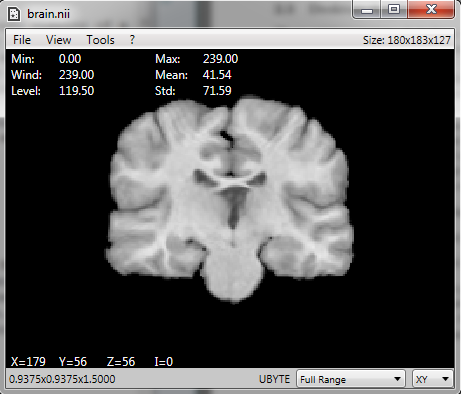
\includegraphics[width=90mm]{..//literatureSurvey/graphics/imview_01.png}
\caption{2D View (left) and 3D View (right)}
\label{fig:UIdesign1}
\end{figure}





\subsubsection{3DSlicer}
\textit{3DSlicer} is a free open source software that provides a modular platform for image analysis and visualization. Of all the packages, this tool seems to be the most feature rich, which is not surprising as it is funded by a number of American organisations such as  the National Alliance for Medical Image Computing, Neuroimage Analysis Center and others. Although it features a wide variety of tools, the focus will be on the ones relevant to this project. \textit{3DSlicer} allows for loading of different files of different formats. It provides options to composite different slices on top of each other for comparison. It supports hardware accelerated volumetric rendering of medical image data. It is widely customisable with global settings. Layouts are also customisable. It has an extensive set of tools for manual and automatic image segmentation. It has an in-built feature to download sample data, which would be a useful inclusion for the web app project. Another powerful feature is that \textit{3DSlicer} allows the addition of new functionality and provides a number of generic features not available in competing tools. All in all, \textit{3DSlicer} appears like a well designed, user-friendly program that has an overwhelming amount of functionality. It will be another good benchmark and inspiration for this project.

\subsubsection{MIview}
\textit{MIView} was programmed by Greg Book, is open source and provides much the same functionality as \textit{MITK}. \textit{MIView} is an \textit{OpenGL} based medical image viewer which aims to support a wide range of medical imaging files such as \textit{NIfTI}, and raster images. The main goal of \textit{MIView} is to provide a platform to load any type of medical image and be able to view and manipulate the image. Volume rendering is also supported. Control-wise, support for mouse-wheel scrolling seems erratic, which makes navigation through the slices more cumbersome. Also the buttons tend to be quite small which also does not improve the user experience. It does not appear to support the loading of multiple files together. A number of predefined color look-up tables are provided.


\subsubsection{ITKSnap}

The final website for this project included a survey that asked users about which medical image viewers they used, if any. ITKSnap came up the most frequently, so a brief review is included here. Development started before the year 2000, is currently being lead in development by Paul A. Yushkevich (University of Pennsylvania) and Guide Gerig (University of Utah) and is supported financially by the US National Institure of Biomedical Imaging and BioEngineering. It is currently in its third major revision.

Upon starting up the ITKSnap application, it is instantly appealing. It features a library of recently viewed files, which is very convenient for repeated use. It offers the ability to save a workspace as an XML file which includes which files are currently being viewed, making it easier to share specfic sessions with other users. This would be a great addition to this project.

The controls follow the standard setup, with panning, zooming and traversing all assigned to the different mouse buttons. Scrolling through the indices is performed by scrolling with middle mouse button. A slider is also provided on each panel for selecting a specific index. There are many options for navigating the slices, which seem well thought and focus on convenience. A button is provided to center the image on a selected cursor position.

In terms of viewers, it offers zoomed-in views with a little thumbnail in the corner of the whole image to show which protion is being examined. When trying out some sample data, the 3D view did not display properly. Interestingly it does not feature many options for adjusting the layout of the viewers, with only a four-panel layout and a single panel layout available. As it has been rewritten with Qt, these features should be very easy to implement.

ITKSnap further impresses with the customisation options for image brightness, contrast and colortable lookups. A wealth of options are available for each component, and a wide number of colortables are provided, which can also be edited. A separate information panel summarises the key data facts about the currently loaded files such as dimensions, voxel spacing and orientation.

The program als offers a variety of tools for segmentation (painting custom labelmaps), with manual and semi-automatic tools provided. It represents a volume of work that would be too ambitious to emulate in a project of only three months.

In conclusion, ITKSnap appears to be the most appealing, focused and well rounded medical image viewing software out of the ones that were researched for this project, due to the wealth of customisation yet convenient design. It has a number of features that would make great additions to the current ScanView program. Unfortunately I came across this specific piece of software quite late so have not had the opportunity to add any of these features. 



\subsubsection{Photoshop}
Looking further afield to some graphical editing software programs, some interesting functionality can be discovered. Adobe's \textit{Photoshop} is well known software for creating and manipulating 2D imagery. When editing an image, the user works with a document. The user can add as many layers as required and edit each layer individually. The layers are composited to form the whole picture. Each layer's opacity and compositing/blending mode can be specified. This could be a worth while to emulate for comparing different medical image files in the web app.


\begin{figure}[ht!]
\centering
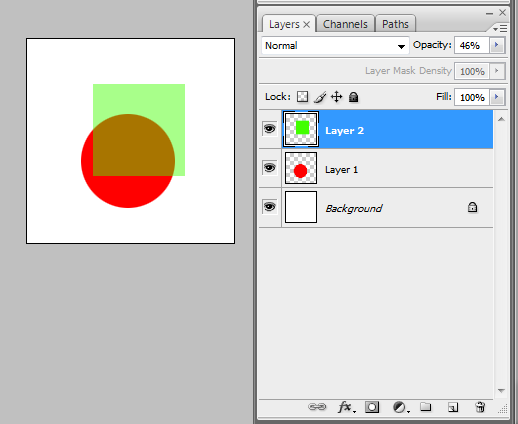
\includegraphics[width=90mm]{..//literatureSurvey/graphics/photoshop_01.png}
\caption{Layer Compositing in Photoshop}
\label{fig:UIdesign1}
\end{figure}


\subsubsection{Nuke}
The Foundry's \textit{Nuke} is a compositing package which is used in the Visual Effects Industry to edit and composite 2D images with each other. It is used among others at high profile Visual Effects companies such as Industrial Light and Magic and Weta Digital\cite{nuke1} \cite{nuke2}). The interface differs from \textit{Photoshop} in that it provides the user with a workplace where any number of nodes can be created. When selecting any node, a graphical display will appear. These nodes can be linked together and do anything from loading a specific image file, transforming the whole node tree or applying an image filter such a film grain. The power of this approach is the modular nature of a tree. Any node can be taken out and reinserted at another place into the tree, thereby changing the final image. Additionally, for comparing different images, by default the software supplies two image buffers which the user can fill with any image of his choice (including of course the result from any node tree in his workspace). Once both buffers are filled, the user can easily toggle between the two images, blend between them by setting the opacity and even use a slider to reveal just a portion of either image. So while \textit{Nuke}'s node-based approach may be overkill for this project, \textit{Nuke}'s image blending seems quite desirable for this project as it would give the user a variety of ways in which he can compare multiple images. 


\begin{figure}[ht!]
\centering
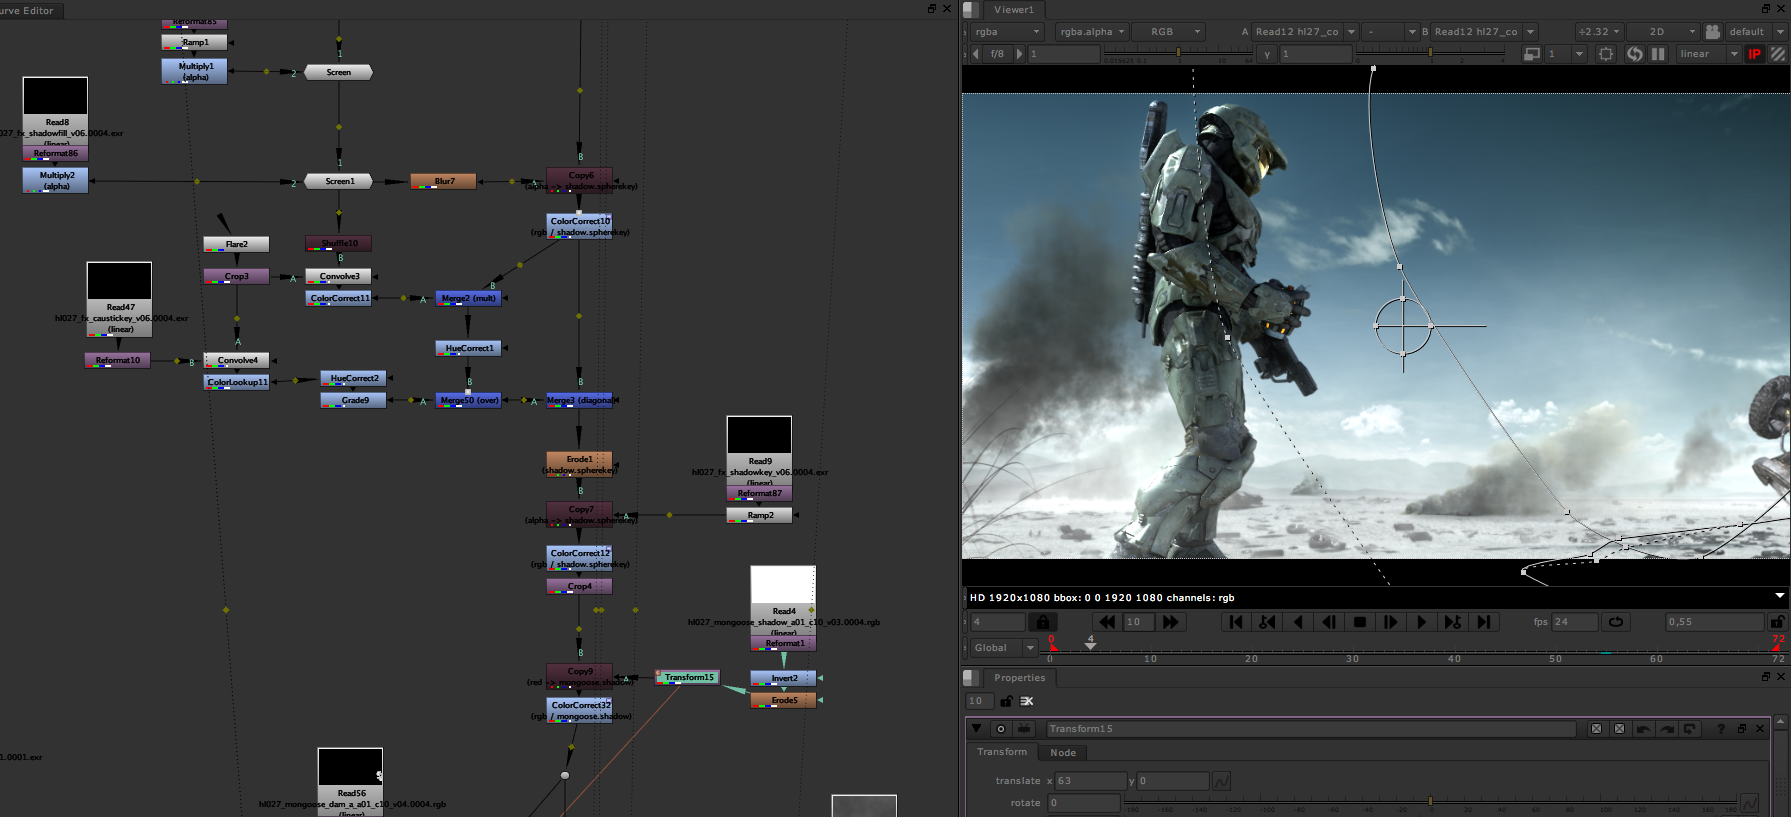
\includegraphics[width=170mm]{..//literatureSurvey/graphics/nuke_02.png}
\caption{Nuke's node-based workspace}
\label{fig:UIdesign1}
\end{figure}


\subsection{Web Applications for Medical Image Viewing}


\subsubsection{Web Framework XTK}

As suggested in the project specification, the goal of this project is to use the \textit{X Toolkit}(\textit{XTK}), a \textit{JavaScript}-based framework for visualizing and interacting with medical imaging data using \textit{WebGL}. It was developed and maintained by Haehn et al of the Fetal-Neonatal Neuroimaging and Developmental Science Center at Childrens Hospital Boston, Harvard Medical School, US (\cite{xtk}). \textit{XTK} provides an API to load medical images, based on \textit{WebGL} technology for displaying 3D graphics and the \textit{HTML5} canvas elements to display 2D components. It hides a lot of the low-level elements of \textit{WebGL} and is designed to load and configure medical image data files of various types (including \textit{NIfTI}). The library is well documented and comes with several tutorials as well as a number of example applications, which will be discussed in the next section. It appears to follow closely the suggestions laid out in section 2.1 (Medical Imaging) in that it provides means to display 2D and 3D slice visualisations (Surface Shaded Display and Volume Rendering are supported), with simple mouse-based controls. It allows for loading of label (segmentation) maps which can overlaid on top of the image data files. It also features color tables (LUTs) to display the data. More advanced features such as reslicing a volume along arbitrary axis and rendering particles are also supported.


The library is comprised of a host of different components. Since it would take too long to explain every class, I will describe the four concepts of renderers, volumes, slices and labelmaps to give an insight into XTK's workings. The XTK website has a list of API commands for these but it is not up to date, and I learned more by actually looking into the code.

A X.renderer is an abstract virtual class and inherits to X.renderer3D and X.renderer2D.  The renderer has a private attribute called topLevelObjects which is an array of X.objects that have no parents themselves. This matters as inherited X.objects such as X.volume have nested X.objects as member attributes. The X.renderer class also has a private objects class, which is an array of all X.objects that are linked to this renderer. Next, an X.loader object is also assigned to the private 'loader' attribute. This loader will be used for any loading of file object, as will be discussed in more detail later in this subsection. The X.renderer class also has an X.camera class. This is used to view the renderer content, and viewing transformations such as panning, zooming and rotation are handled by this class. There exists an inherited 2D and 3D camera class. Then there is an X.interactor assigned as well. This class handles all mouse and keyboard inputs. 

The inherited X.renderer2D class has extra attributes to specify which slice is being rendered, such as currentSlice, orientiation, sliceHeight and sliceWidth. It has a framebuffer array attribute which stores the current slice texture information which will be rendered to screen. It also has a labelFrameBuffer which is secondary buffer that is used to render a labelmap if one has been loaded. This is in essence an A over B compositing effect. The X.renderer3D class has different internal attributes since it does its drawing through WebGL technology. It contains number attributes of the the dimensions of the loaded objects, as well as an X.shaders object and various buffers of the form goog.structs.Map to store vertex, normal, color and texture information of the currently loaded objects.

There are various methods in the X.renderer classes. Init(), render() and update() warrant a closer look. The init() function is called in the beginning to set up main aspects such as the X.interactor, X.camera, X.loader, HTML Canvas and Context on which to draw on. The render() function deals with the actual drawing of content onto the canvas. The renderer3D and renderer2D classes naturally differ in their implementations of this function, but both call on the parent's render() function to continuously redraw the frame. Renderer2D.render() function reevaluates if the current buffer needs to be recalculated and if so does it inside the scope of the code, whereas the renderer3D.render() function pushes any changed data to the GPU for drawing. SOMEWHAT HAZY UNDERSTANDING OF THIS, IMPROVE.


\begin{figure}[ht!]
\centering
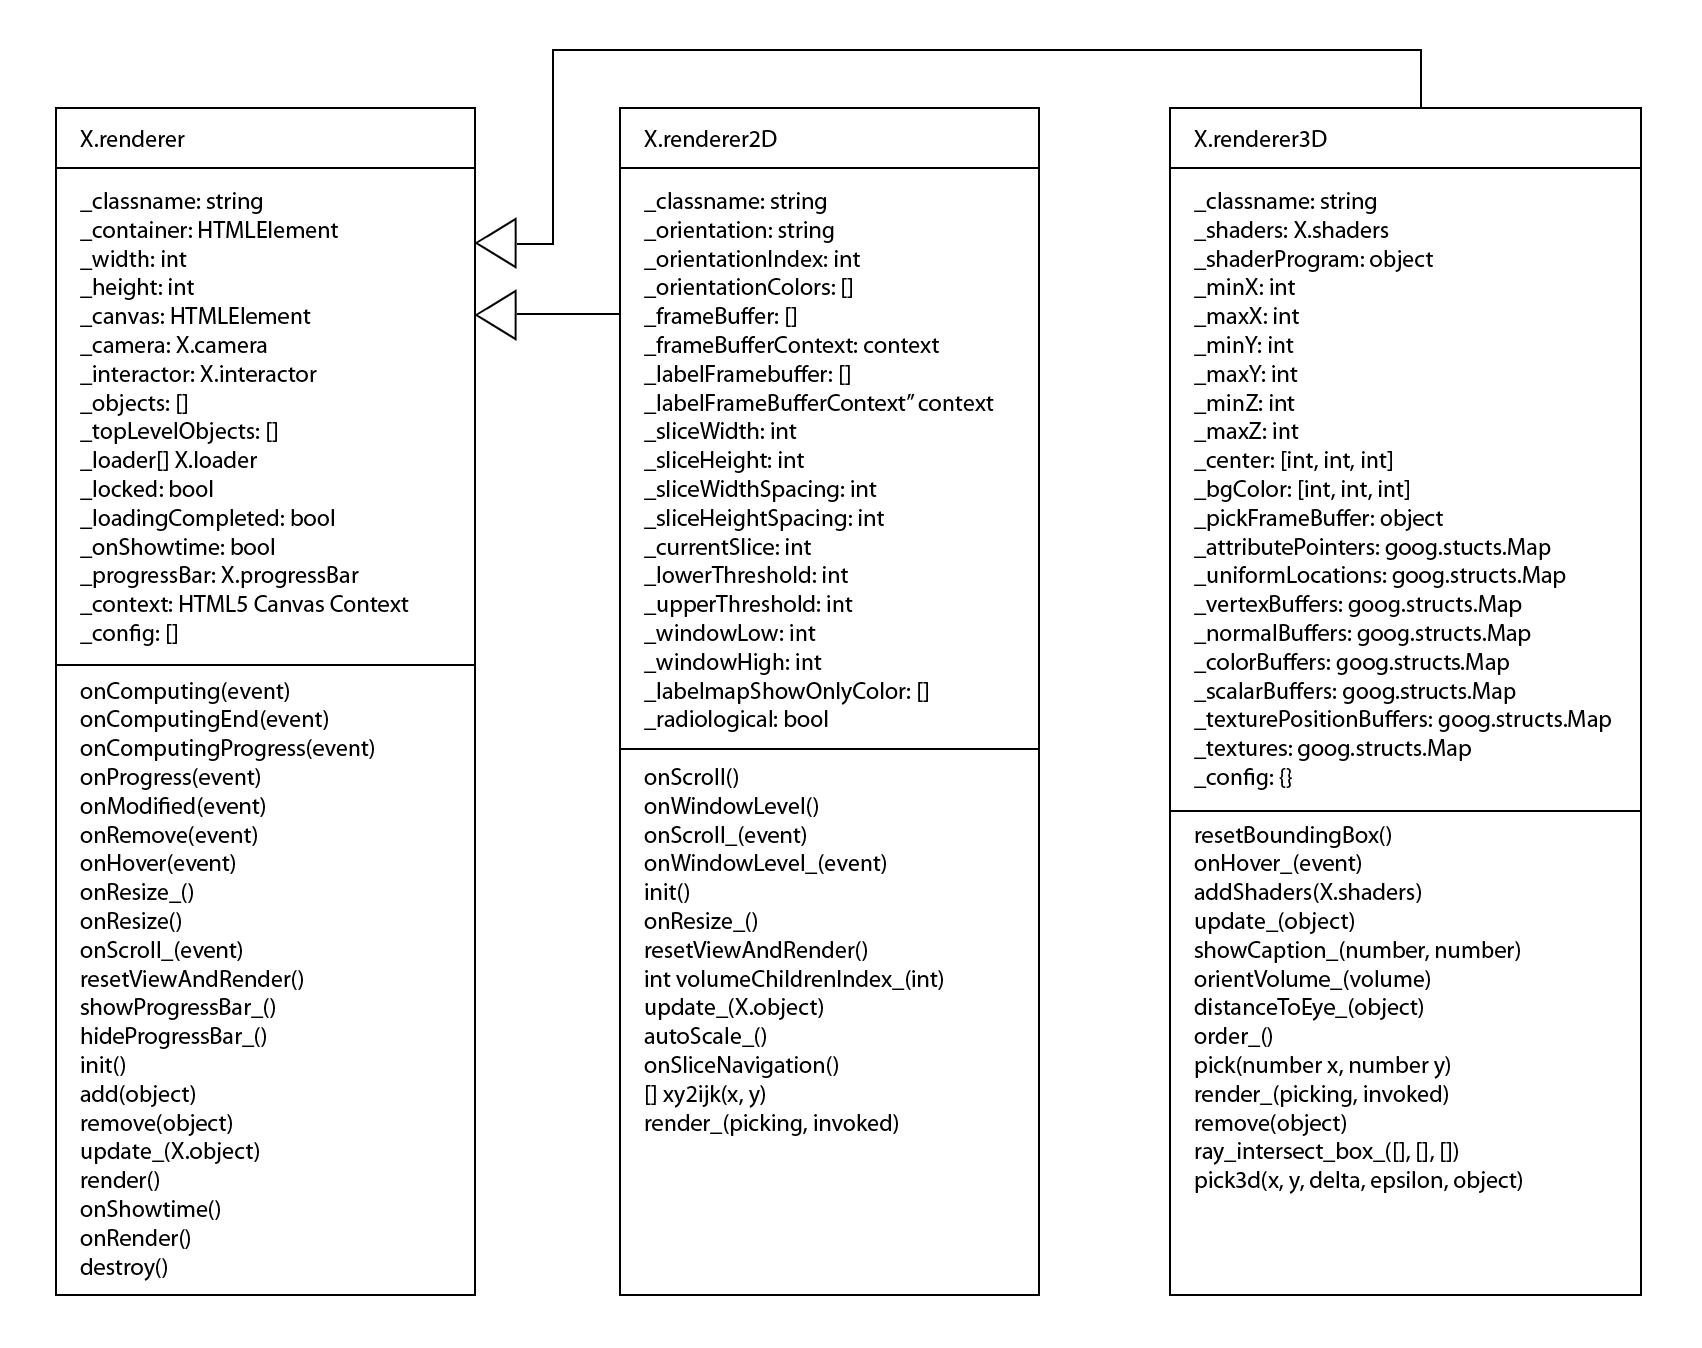
\includegraphics[width=170mm]{graphics/xtkUML_01.png}
\caption{Full Class Diagrams for renderer.js, renderer2D.js and renderer3D.js}
\label{fig:UIdesign1}
\end{figure}


X.slice is a type of X.object and inherits a host of attributes and functions from it (see below for UML diagram). It stores attributes for a current slice, such as orientation vectors (\_front, \_up, \_right), \_center, dimensions (\_width and \_height).

Generally, XTK uses the concept of injections to add extra features into various X.classes. A selection can be see in Figure 34. X.loadable supplies attributes to store file data. X.displayable offers several attributes useful for displayin in Canvas, such as \_color, \_points and \_texture. Finally, X.thresholdable enables the setting of different threshold values, as is used in the X.volume.

The Xvolume is a more complex type of Xobject. As it is an X.object, it can be added to a X.renderer and inherits all the attributes and methods from the X.object class. Volumes are also injected with the loadable.js code and thresholdable code. An X.volume has a variety of attributes that deal with the currently loaded data, such as current indices (\_indexX, \_indexY and \_indexZ), range which specifies the maximum indices. It has \_windowLow, \_windowHigh, \_thresholdLow and \_thresholdHigh (the last two from thesholdable.js) which dictate the window and treshold settings. As for all attributes that are to be accessed from outside the API, setter methods have been written which take care of internal logic. It is the setter methods for window and threshold that are being called through the Levels Panel when adjusting the sliders. The X.volume has the inherited array children from (X.object) in which it stores all the precomputed X.slices. A precomputed X.slice is generated when the slice index is set to an index that has not been visited yet since instantiation. In this way, the X.volume will buffer more and more slices throughout scrolling. Once the X.slices have been buffered, lookup is noticeably quicker. When the X.volume is set to an uncomputed sliceIndex, different functions are called than when a precomputed slice is present, including forcing a redraw in the render.js class. 


So when loading a custom labelmap, I had to implemented a method to clear the \_children array.

\begin{figure}[ht!]
\centering
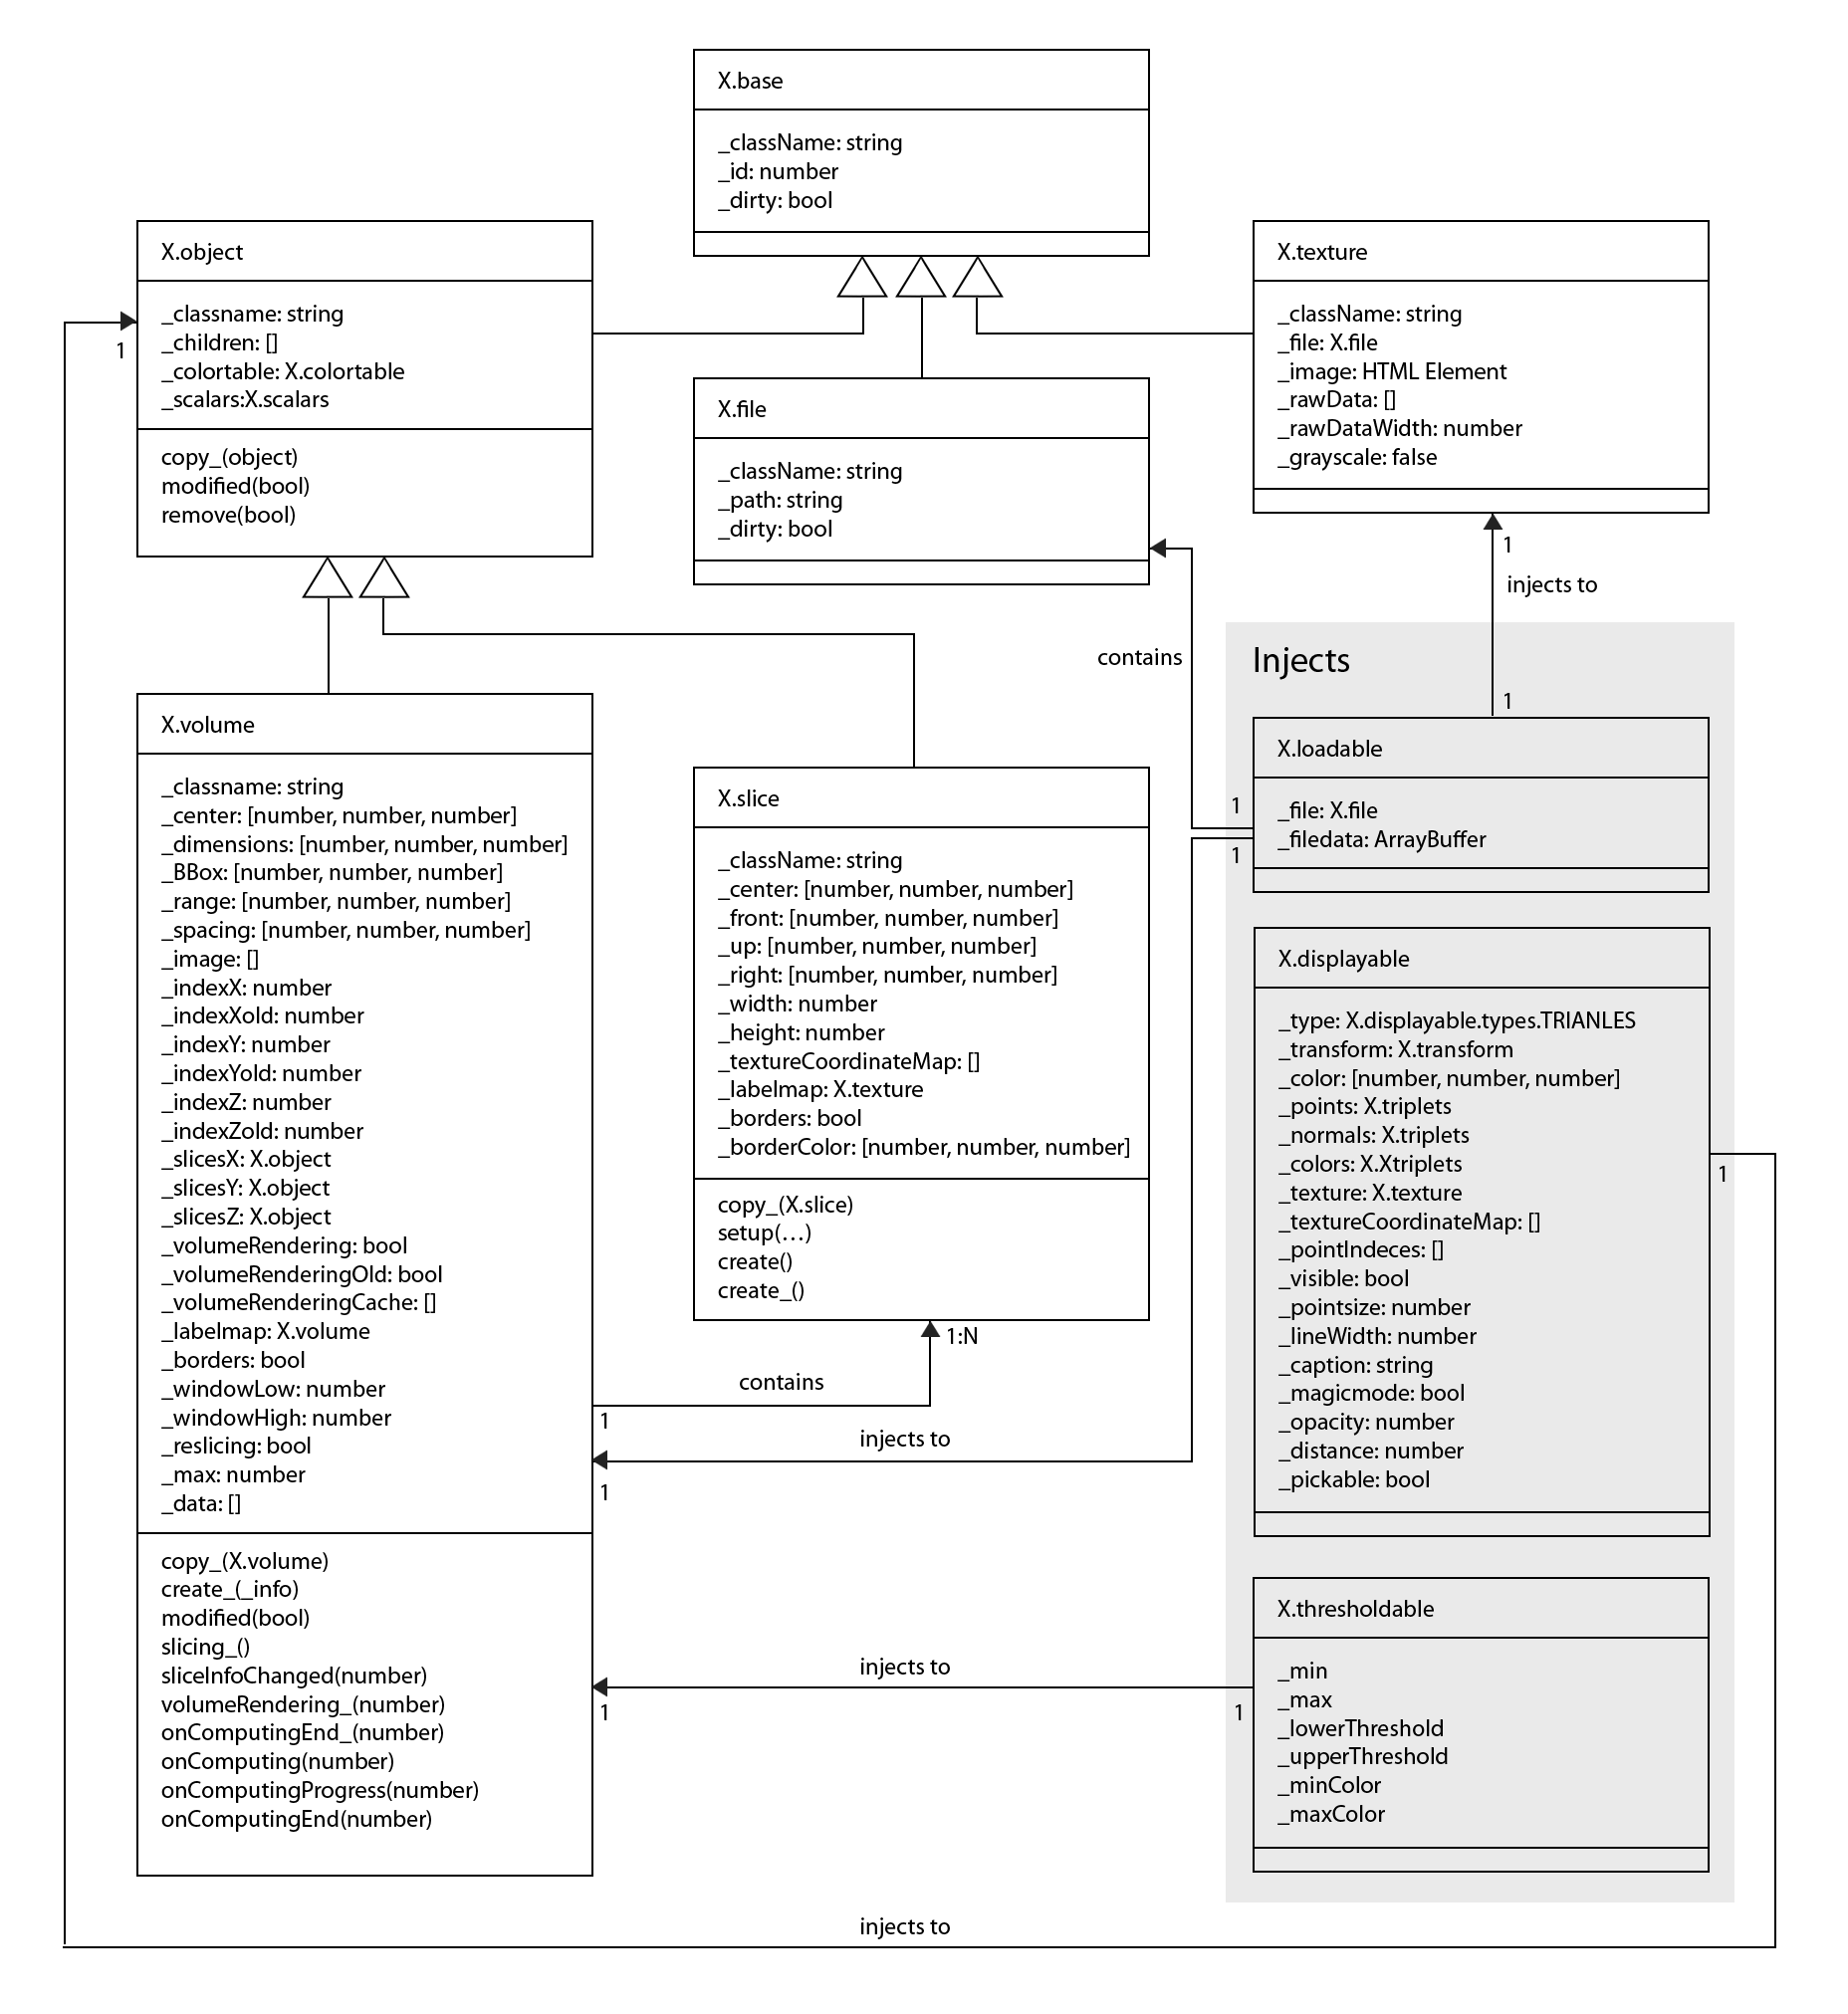
\includegraphics[width=170mm]{graphics/xtkUML_04.png}
\caption{UML Class diagram for X.volume and dependencies}
\label{fig:UIdesign1}
\end{figure}



The \textit{XTK} library also provides a module for creating User Interface (UI), that can be overlaid on top of the image viewers, with easy controls to connect the image content with the UI controls.
The popular forum for coding questions Stackoverflow hosts about 100 questions regarding \textit{XTK} to date, and occasionally the \textit{XTK} developers offer up answers.


\subsubsection{SliceDrop}
The \textit{XTK} library also provides links to example applications. One of these is \textit{SliceDrop}\cite{slicedrop} which has written by the \textit{XTK} developers and appears to be a testing bed for many of \textit{XTK}'s features as it is often referred to on the \textit{XTK} Stackoverflow forums. It provides part of the desired functionality and shows off the possibilities provided by \textit{XTK}, but also outlines some of its short comings. Like the desktop software \textit{MITK}, the user can load a file and view it in the standard 4 views, split into 3D and 2D windows. The layout of these views is somewhat customisable, although not to the extent of the \textit{MITK}. The user can interact with the images by scrolling the mouse wheel, which changes the index of the current slice. An interesting feature which has been added lately is the incorporation of popular file sharing site \textit{DropBox} to allow users to share files more easily across the internet.

There appear to be some bugs in \textit{SliceDrop}. When loading \textit{NRRD} files, as the image is offset and not centered. The image brightness controls seem not calibrated correctly, as with little mouse interaction, the brightness will clamp to white or black and can not be reset other than restarting the program (refreshing the page for web-apps). Furthermore the app does not allow to load custom labelmaps. Also the viewers provide some functionality which is not clearly communicated to the user, such as holding the 'shift' button and move the mouse will adjust the slice index of the other viewers. In general \textit{SliceDrop} has less than the minimum functionality required for this project, but shows the potential of the \textit{XTK} library. 


\subsubsection{Brainbook}
\textit{Brainbook}\cite{brainbook} is a web-app which builds on and extends the features of \textit{SliceDrop} by adding painting tools. It allows the user to paint onto a given file with a standard brush a number of auto selection tools which will fill out a region in 2D or 3D space. The web app offers to save the file, but at time of writing this feature was not working correctly. Since heavily based on \textit{SliceDrop}, it features similar advantages and disadvantages, but provides the painting functionality that is desirable for this project. Therefore it should be of benefit to study this implementation.

\subsubsection{DWV - DICOM Web Viewer}
This viewer does not provide much functionality other than scrolling through one stack of slices. The user interface is sparse and does not give sufficient feedback to the use of what is currently happening. It uses the \textit{HTML5} Canvas element to display the file contents.

\begin{figure}[ht!]
\centering
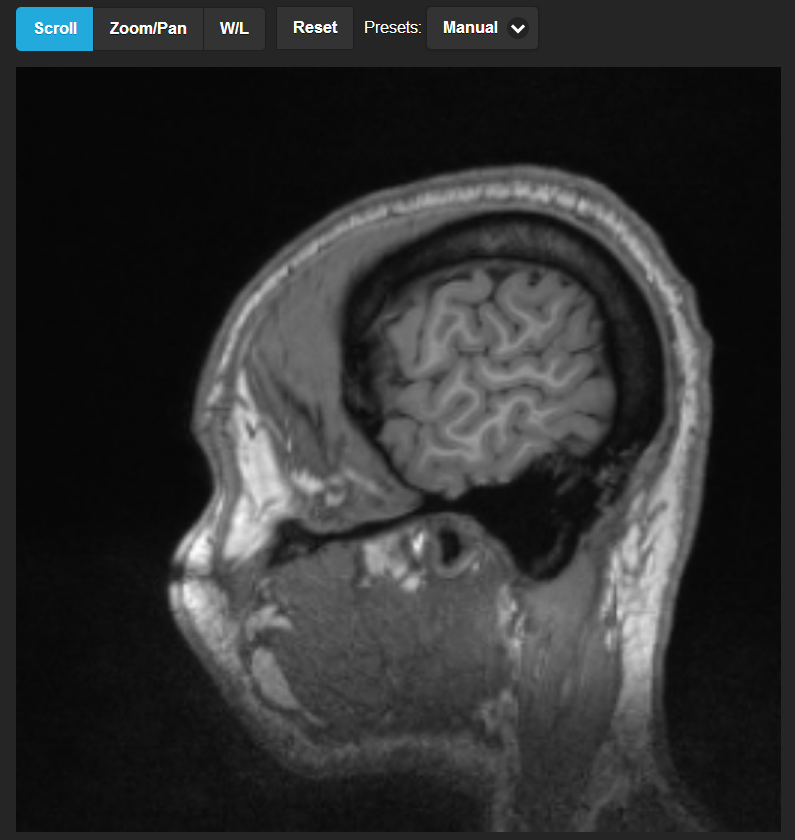
\includegraphics[width=90mm]{..//literatureSurvey/graphics/webViewer_01.png}
\caption{DMV User Interface}
\label{fig:UIdesign1}
\end{figure}



\subsubsection{Papaya}
Papaya\cite{papaya} is a \textit{JavaScript}-based medical image viewer with limited functionality. It has a clean uncluttered design, is easy to use and gives good visual feedback to the user. It successfully adheres to the user control guidelines outlined in section 2.1. It only displays 2D views of slices and does not allow any customisation in terms of label maps, windowing or compositing. It also uses the \textit{HTML5} Canvas element to render the 2D data.

\begin{figure}[ht!]
\centering
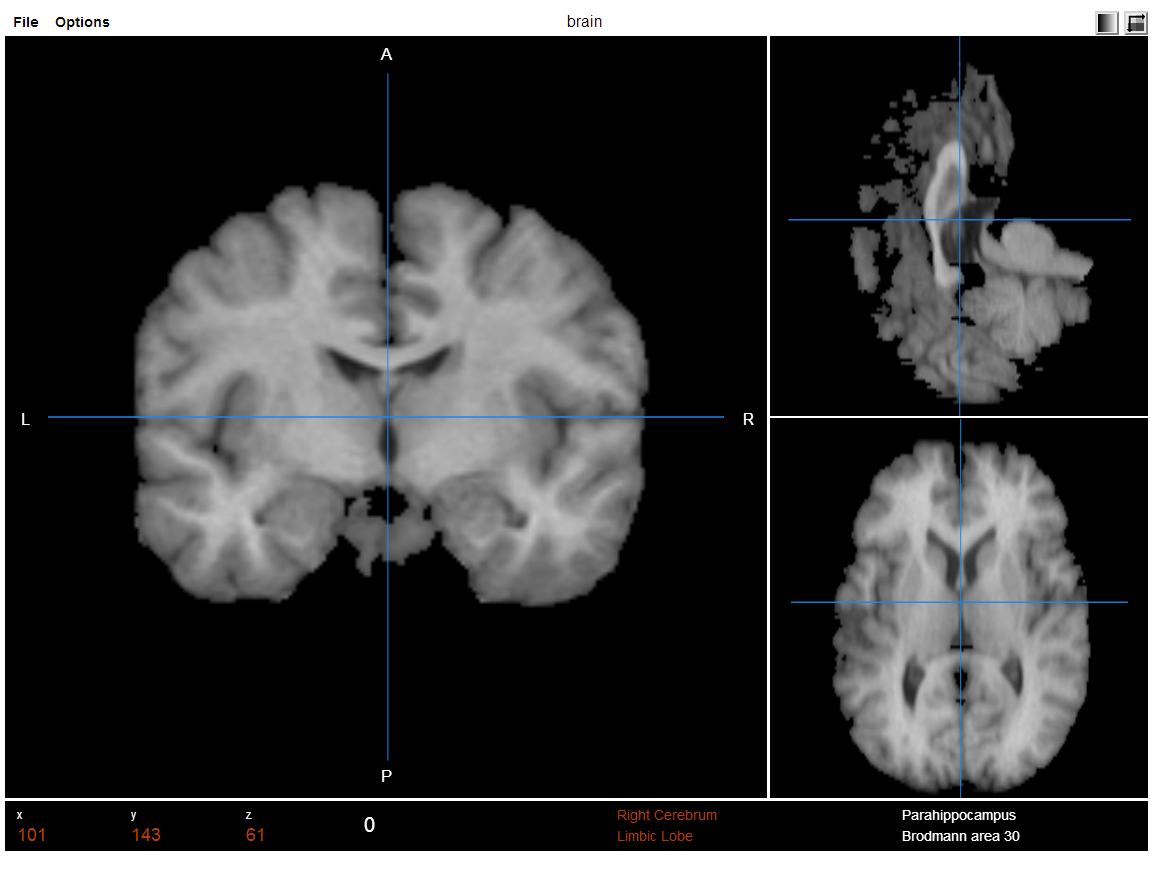
\includegraphics[width=90mm]{..//literatureSurvey/graphics/webViewer_02.png}
\caption{Papaya User Interface}
\label{fig:UIdesign1}
\end{figure}



\subsubsection{Other}

The website \url{http://www.idoimaging.com} lists a number of other available browser-based viewers.


\subsection{Developing Web Applications}

\subsubsection{Web Browsers}

According to Web Browser usage statistics from w3counter.com for 2014, the 4 most used
browsers are (in descending order) Chrome, Internet Explorer, Firefox
and Safari. Chrome leads with 38.5\% market share, followed by Internet Explorer (21.2\%), Safari (15.4\%), Firefox (15.2\%) and Opera (3.1\%)- REFERENCE FROM WEBSITE.

\begin{figure}[ht!]
\centering
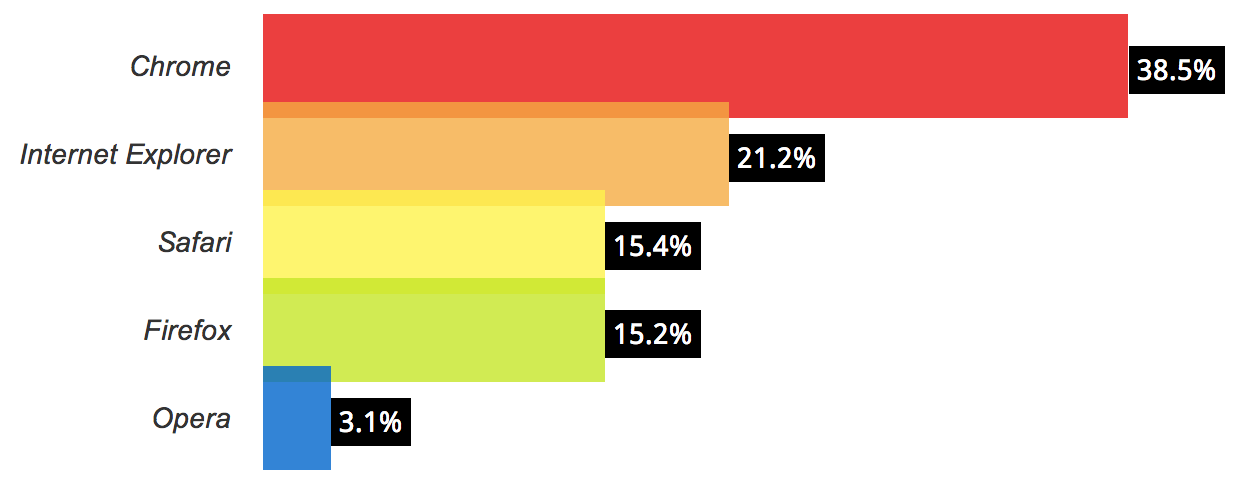
\includegraphics[width=170mm]{graphics/webStats_01.png}
\caption{Browser Market Share July 2014 - REFERENCE}
\label{fig:UIdesign1}
\end{figure}

Looking at a breakdown over the last 10 years, Internet Explorer used to be the most used Web Browser in 2007 with 67.6\%, but its dominance has steadily declined up until the present day. In the same time span Mozilla's Firefox gained popularity and its market share peaked in 2010 but also decreased afterwards to equal Safari's market share in July 2014. Safari's market share has stayed relatively constant until it more than doubled in 2012 (possibly linked to the rise in IOS devices like Apple's IPhone and IPad around 2012 REFERENCE). Google's Chrome Web Browser rose steadily from 2009 onwards and beat Internet Explorer in 2012 to become the most used Web Browser at present time.

\begin{figure}[ht!]
\centering
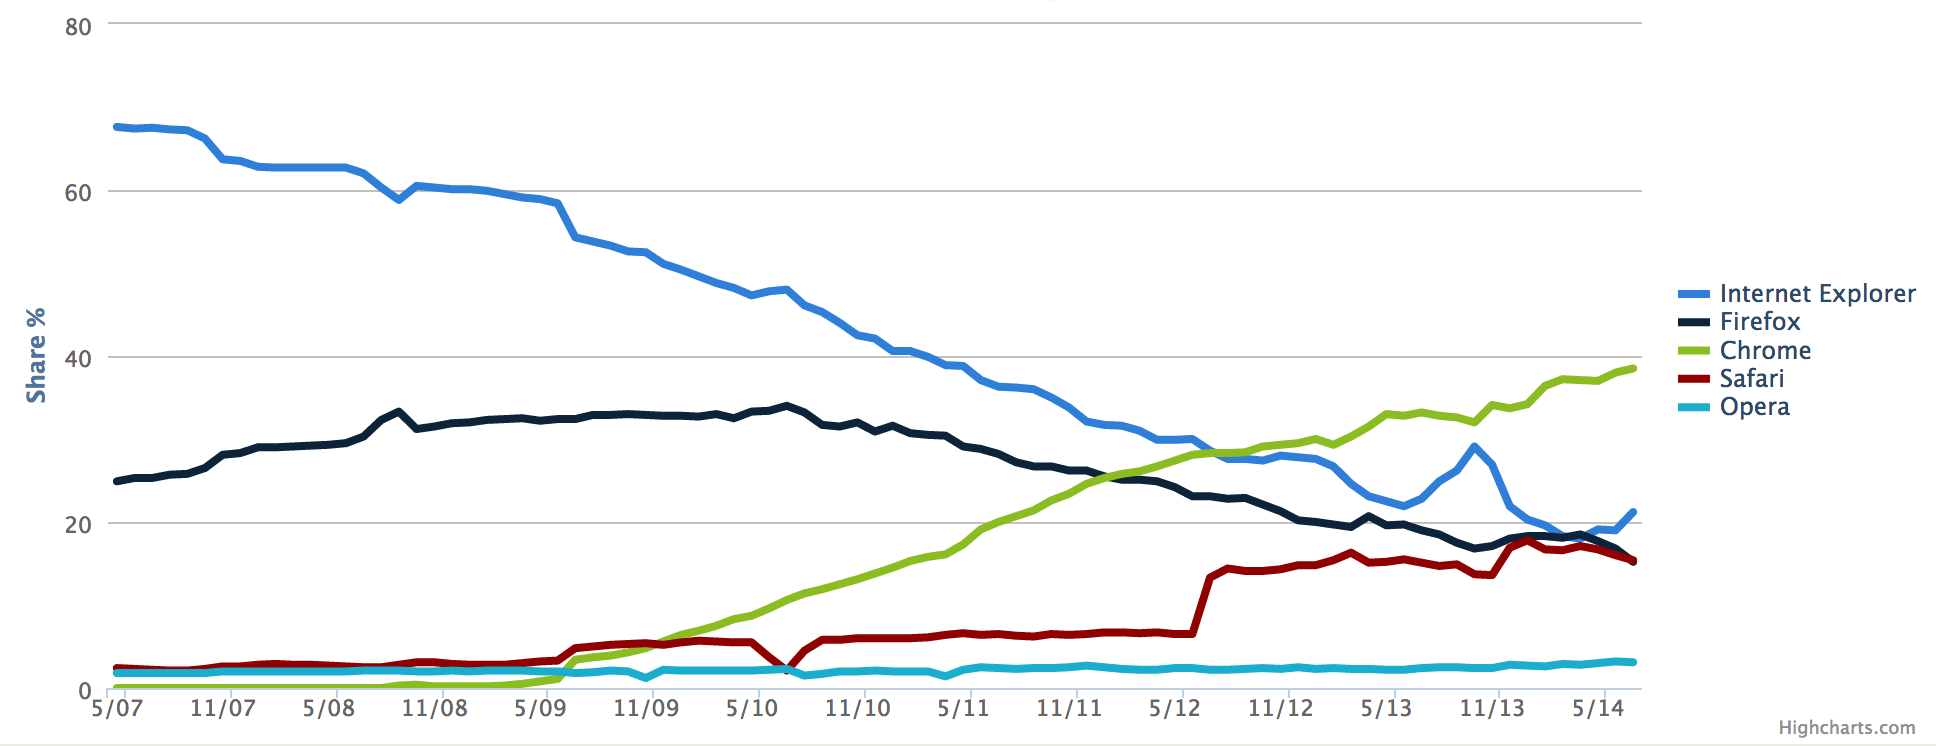
\includegraphics[width=170mm]{graphics/webStats_02.png}
\caption{Browser Market Share History - REFERENCE}
\label{fig:UIdesign1}
\end{figure}

The site www.w3schools.com, a popular tutorial site for web programming, has slightly different statistics. Chrome still comes out on top with 59.8\%, but the places for Firefox and Internet Explorer are reversed with 24.9\% and 8.5\% market share respectively. W3School's sample set comes from people logging onto their sites, so therefore are more likely to be developers rather than casual users. This could mean that developers prefer Chrome and Firefox (a group where I would include myself).

\begin{figure}[ht!]
\centering
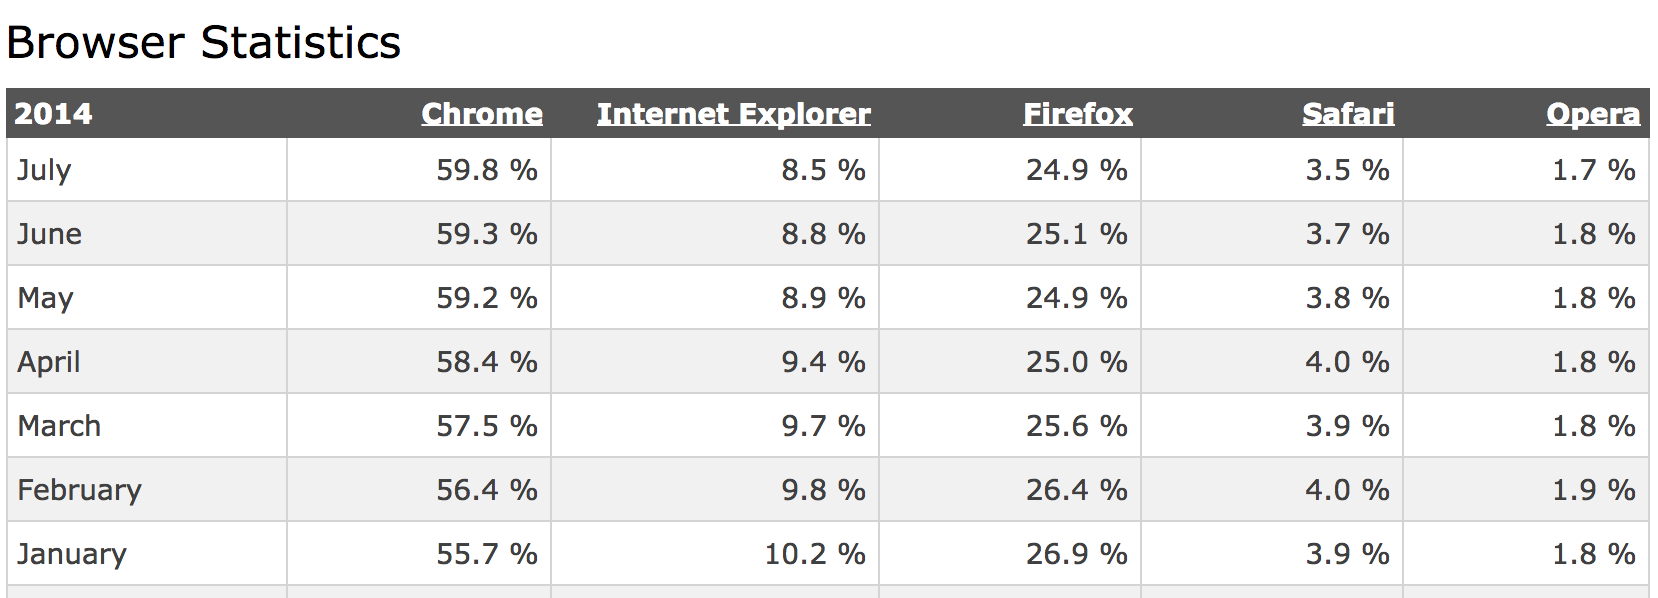
\includegraphics[width=170mm]{graphics/webStats_01b.png}
\caption{Browser Market Share 2014 - REFERENCE}
\label{fig:UIdesign1}
\end{figure}



\begin{figure}
\centering
\begin{subfigure}{.5\textwidth}
  \centering
  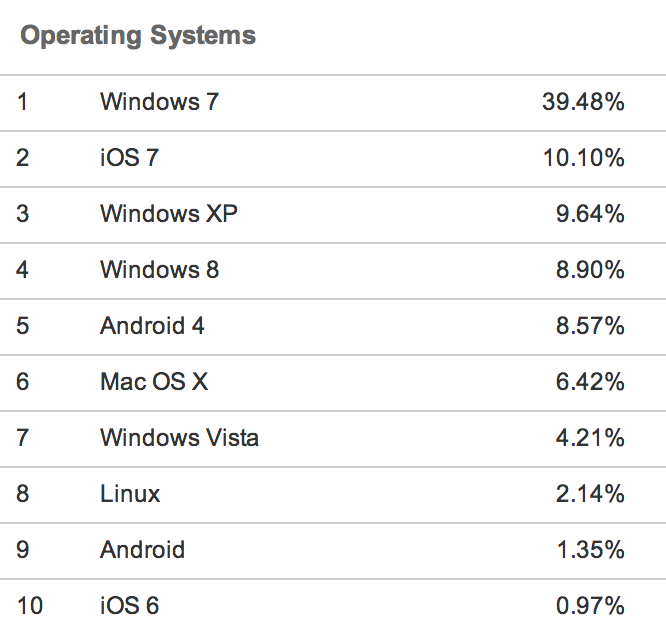
\includegraphics[width=80mm]{graphics/webStats_03.png}
  \label{fig:sub1}
\end{subfigure}%
\begin{subfigure}{.5\textwidth}
  \centering
  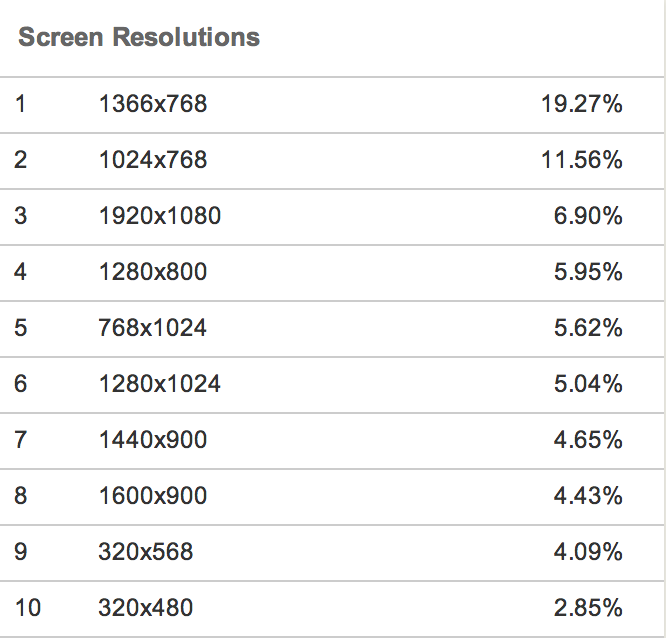
\includegraphics[width=80mm]{graphics/webStats_04.png}

  \label{fig:sub2}
\end{subfigure}

\caption{Most used Operating Systems (left) and Screen Resolutions (right)}

\end{figure}

Further statistics from w3c show that most Web Browser usage comes from Windows 7 (39.48\%) followed by iOS 7 (10.10\%) and Windows XP (9.64\%). Most used screen resolution is 1366x768 pixels (19.27\%).

Given the statistics discussed above, it was decided to mainly develop for Google's Chrome. The other browsers will be supported as secondary priority. It will be developed and tested on Windows 7, OSX Mavericks and Linux Ubuntu, which should cover most computer Operating Systems. In terms of screen resolution, the most widely-used screen resolution of 1366x768 will be taken into account, but a higher resolution assumed, such as 1920x1020. This is obviously an important issue, since a screen with HD resolution (1920 x 1080) and a screen with a smaller resolution of 1366x768 will need to have differently sized components. Therefore using absolute pixel values, such as setting a button or section to be exactly X pixels wide could cause problems, and care will have to be taken to make the website workable across different resolutions.




\subsubsection{Developing websites}

There are many ways to make a website. At a very basic level, a website can be written with just HTML (Hyper Text Markup Language) code. HTML is written with tags as in the example below. This code is converted into a tree format of\textit{JavaScript}node objects or Document Object Model (DOM) by the Web Browser. The purpose of this is to provide a programmatic interface for scripting (removing, adding, replacing, eventing, and modifying) this live document using\textit{JavaScript}[REFERENCE]. The nodes come in different types. These nodes can also be created by running\textit{JavaScript}methods such as the createElement() function. The point is that\textit{JavaScript}and HTML are linked very closely.

\begin{verbatim}
<html>
    <body>
        Hello World
    </body>
</html>
\end{verbatim}

Creating websites with just HTML however is not quite enough in today's world of modern web development. Modern websites can be thought of as a combination of structure, style and interactivity [REFERENCE]. These three jobs are handled in turn by HTML, CSS and JavaScript, which go hand in hand to deliver modern web page content. CSS was first published and recommended by the W3C in 1996. It is generally used to style the look of HTML content. This was previously possible with HTML, but involved a lot of work as elements had to be type set individually and was still relatively limited compared to what is possible with CSS today. With CSS an element could be assigned a class, which would refer to specific set of CSS rules.

\begin{figure}
\centering
\begin{subfigure}{.5\textwidth}
  \centering
  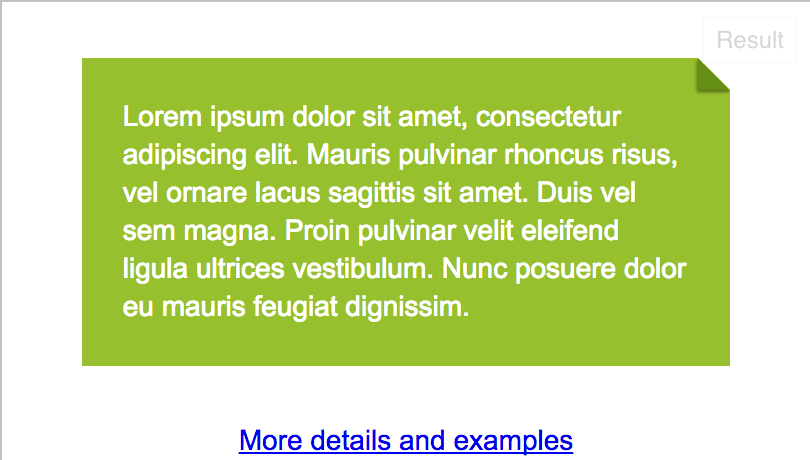
\includegraphics[width=82mm]{graphics/css_01.png}

  \label{fig:sub1}
\end{subfigure}%
\begin{subfigure}{.5\textwidth}
  \centering
  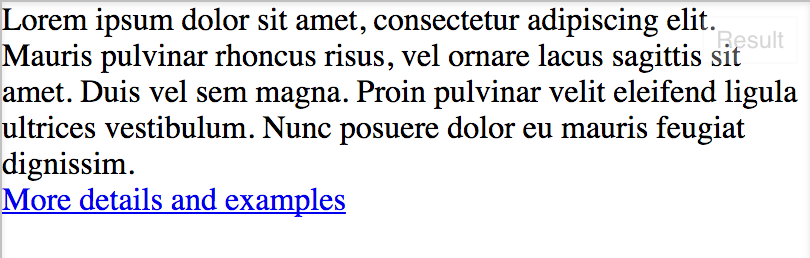
\includegraphics[width=82mm]{graphics/css_02.png}

  \label{fig:sub2}
\end{subfigure}
\caption{HTML with CSS (left) and without CSS (right)}

\end{figure}


Additionally\textit{JavaScript}can be include as code itself in an HTML document with the <script> tag. See the example below.\textit{JavaScript}is used to add functionality to a website by managing interactive elements, function calls and whatever else a developer can think of doing with it. Advanced features such as WebGL and HTML Canvas are manipulated with JavaScript. When a website contains JavaScript, it is downloaded to the user's local machine and run locally ('client side') by the Web Browser's\textit{JavaScript}interpreter. With increasing computational power of machines and faster processing speeds of\textit{JavaScript}by Web Browsers, complex code can be run locally and does not rely on network speed.



\begin{verbatim}
<script>
    document.write("Hello, World!");
</script>
\end{verbatim}


In terms of organisation, it is possible to include the code from all three language in one base HTML file, but this is extremely undesirable as it lacks modularity and will be hard to test and debug. Instead, it is convenient to keep each type of language to separate files. This makes everything more modular, easier to edit, and individual components will be easier to update or swap out. Methods on dealing with more complex bodies of code will be discussed in a later section.




\subsubsection{Web Browser Compatibility}

To make things more challenging, various programming aspects such of HTML, CSS,\textit{JavaScript}and DOM functionality are supported to varying degrees in the different Web Browsers and versions. This stems from the fact that Web Browsers are created and maintained by different companies (with differing business goals and implementation strategies). In the late 1990's this proved disasterous as Web Browsers with different features existed without any coordination between them. However with the creation of the World Wide Web Consortium, the main international standards organization for the World Wide Web, matters took a turn for the better. The organisation is lead by Tim Berners-Lee, the inventor of the World Wide Web, and sets out the standards used for Web Browser scripting, such as CSS, HTML,\textit{JavaScript}and many more. This happened in several stages and revisions over the years, and is now probably more unified than ever before. 

However there still remain small differences, which is only natural when different companies are maintaining these different browsers. For example, WebGL has been supported by Google Chrome since Februray 2011, whereas it was only introduced to the Internet Explorer with Version 11, which came out in October 2013. Also, not all CSS features, used for styling the look of a website, are universally supported or at least support is lagging behind between browsers. For example when searching for the CSS property "box-shadow" www.w3schools.com will list which browsers and versions support this attribute. Luckily the most commonly used elements tend to be supported across all browsers. The http://www.quirksmode.org/ website aims to provide a comprehensive breakdown of provided features across different browsers. Another issue is that the Web Browsers'\textit{JavaScript}interpreters can differ in their implementation.

\
It is anticipated that all the variations will become a source of problems when developing the project and some time will have to be dedicated to test and if necessary reimplement certain sections of the code that does not run successfully in all browsers. A method called 'browser sniffing' could be employed, where the type and version of Web Browser is determined and the code configured accordingly. However W3C does not recommend this, as there would be too many variations to cater for. Instead they advocate using feature detection, which allows the developer to query for support of a feature such as WebGL instead of having to check the browser version when WebGL was first supported. This is more elegant and future-proof. 
Looking at this from a code perspective, detecting a browser and version is done by the "navigator.userAgent"\textit{JavaScript}command. It returns a string like:

\begin{verbatim}
Opera/9.80 (Macintosh; Intel Mac OS X 10.6.8; U; Edition Next; en) Presto/2.10.289 
Version/12.00
\end{verbatim}

This string can be parsed, but will obviously differ widely for each different browser. It is also error prone, depending on the string parsing method employed and assumptions made about the format of the string. Instead, detecting a feature would be done like so:
\begin{verbatim}
if(!!document.createElement('video').canPlayType === true) {
  // run some code that relies on HTML5 video
} else {
  // do something else
}
\end{verbatim}

Testing for features like this seems a better approach since you are directly testing for a feature that you are using. Also it is independent of specific browser types and versions.

Web Browsers for mobile devices add another layer of complexity to this, but will be ignored for the scope of this project.




\subsubsection{Web Frameworks for Single Page Apps}

The aim of this project is to create a singe-page application (SPA), which loads into the browser on the client side and does not require complete page refreshes [REFERENCE].

As goes for any body of complex code, an orderly and modular structure should be implemented and maintained. The estimated length of code for this project lies in the tens of thousands of line code and a multitude of classes. Therefore, it is in no way feasible to just include the\textit{JavaScript}in script tags in the actual HTML pages. A more avanced solution is needed.

Thankfully, this requirement for advanced code structuring was generally recognised, and a dominant solution to this issue by the name of Model View Controller (MVC) pattern has emerged. MVC separates the concerns in an application into three parts [REFERENCE]:

\begin{itemize}
\item Models represent the domain-specific knowledge and data in an application, such as specific data container classes. Models can notify observers when their state changes.
\item Views typically constitute the user interface in an application (such as markup and templates), but not necessarily so. They observe models, but do not directly communicate with them.
\item Controllers handle input (clicks or user actions) and update models.
\end{itemize}

So in an MVC application, user input is handled by controllers, which then updates various models. Views listen to the state of models and update the user interface or visual front end when changes are detected. The definition of MVC frameworks is not always followed strictly and some merge the role of controller and views into one. BackboneJS, which will be used for this project does exactly this. For that reason, these more loosely defined implementations are sometime called MV* frameworks. It would in theory be possible to organise the code for this project in a custom MV* pattern, but libraries such as Backbone are well established and reduce a lot of tedious work that would otherwise be required. AngularJS, CanJS EmberJS are other popular MVC implementations.

\begin{figure}[ht!]
\centering
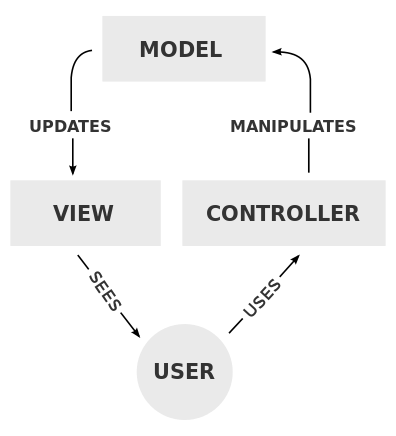
\includegraphics[width=70mm]{graphics/MVC_01.png}
\caption{A typical interaction of MVC components REFERENCE-WIKI}
\label{fig:UIdesign1}
\end{figure}


At the time of writing, the \textit{Backbone} library seems to be a good choice to manage the complexity and structure of the project. It was written by Jeremy Ashkenas and is designed for developing SPAs, and for keeping various parts of web applications synchronized. It has been used by big companies to create nontrivial applications, such as Walmart, SoundCloud, and LinkedIn. I have also used it in successfully in a previous group project. In accordance with the MV* pattern, Backbone provides Events, Models, Collections and Views. Models represent the information in class-like structures, Collections are lists of Models and Views handle the visual representation on the actual HTML site. Finally Events are used to keep track of state changes across the website elements, models and views. It builds on \textit{jQuery} and \textit{Underscore.js}, both libraries which simplify dealing with \textit{HTML} elements. It also provides inheritance for its models, collections and views.

Regarding the design aspect, it looks like twitter-bootstrap.js supplies a convenient library for creating visually pleasing user interface elements. This will cut down on having to spend time to design custom elements with \textit{CSS} and \textit{JavaScript}. \textit{Bootstrap.js} supplies buttons, drop-down menus and commonly-used icons. Some specific UI control elements are not provided by \textit{Bootstrap.js}, so \textit{jQueryUI} will be used. It enables the creation and customisation of complex elements such as slider elements with multiple slider tabs, which will allow for a better user experience. Also, it's dependent on the \textit{jQuery} library which is already being used for \textit{Backbone}.

As this project will make of several modules, it will be important to manage the dependencies of the modules. For example \textit{Underscore.js} and \textit{jQuery} will need to load before \textit{Backbone.js} is used. \textit{XTK} and twitter-boostrap are additional modules that will have to be loaded. \textit{RequireJs} is a \textit{JavaScript} library that provide the ability to asynchronously load nested dependencies. Traditionally \textit{JavaScript} files or modules are loaded sequentially, where the order matters in case a module depends on another module. Additionally it will be helpful to manage the different HTML templates required for the various elements of the web app. \textit{RequireJs} will make it possible to split up everything into neat modules and templates and facilitate testing of all the components.



\subsection{Graphics for Web Applications}

In order to create an interactive Web Browser application that provides graphical feedback, the available tools for creating 2D and 3D graphics in a Web Browser have to be considered. Generally, in the past Web Browsers have provided several different methods to display 2D and 3D graphics on screen, and only recently with the introduction of \textit{HTML5} and \textit{WebGL} has a widely-conformed standard emerged.

\textit{HTML5} is the fifth revision of the HTML standard. \textit{HTML5} introduced a number of important features that were designed to facilitate including and handling multimedia and graphical content on the web without the use of proprietary plugins and APIs. One of these new features is the Canvas element, a scriptable graphical display element which is a low level, procedural model that updates a bitmap element. It was originally introduced by Apple \cite{canvas} . This components forms the basis for most complex rendering of 2D and 3D graphics in modern browser applications.

\subsection{2D Graphics}

Displaying 2D graphics has long been an integral part of Web Browsers. Various aspects and methods allow for the generation and manipulation of 2D graphics in a Web Browser. Aside from simply displaying an image file, there are various other aspects and methods allow for the generation and manipulation of 2D graphics in a Web Browser

\textit{CSS}, as discussed, is used to alter an element's style property, but this is not really suitable for creating intricate 2D graphics, as it is typically used to style the look of \textit{HTML} elements. There are no custom draw commands.

Scalable Vector Graphics (\textit{SVG}) is like \textit{HTML} for graphics\cite{svg}. It is a markup language for describing all aspects of an image or Web application, from the geometry of shapes, to the styling of text and shapes, to animation, to multimedia presentations including video and audio. It is fully interactive, and includes a scriptable DOM as well as declarative animation (via the SMIL specification). It supports a wide range of visual features such as gradients, opacity, filters, clipping, and masking.
The use of \textit{SVG} allows fully scalable, smooth, reusable graphics, from simple graphics to enhance \textit{HTML} pages, to fully interactive chart and data visualization, to games, to standalone high-quality static images. \textit{SVG} is natively supported by most modern browsers (with plugins to allow its use on all browsers), and is widely available on mobile devices and set-top boxes. All major vector graphics drawing tools import and export \textit{SVG}, and they can also be generated through client-side or server-side scripting languages.

Finally, the Canvas API is a client-side scripting technology to allow for the rich creation or alteration of raster images (bitmaps) . It uses vector-based programmatic methods to create shapes, gradients, and other graphical effects, and because it has no DOM, it can perform very quickly. Dedicated scripters can develop games or even full-featured applications using the Canvas API, alone or integrated into \textit{HTML} or \textit{SVG}. It is supported natively in most modern browsers (with script libraries extending support to all major browsers), and even on some mobile devices.

Before the Canvas API became common place, there were different Web Browser plug-ins which would display more interactive graphics and videos. Adobe's \textit{FlashPlayer} and JavaApplets were very common for this purpose.



\subsection{3D Graphics}

\subsubsection{Pre-WebGL}

3D Graphics are usually defined by a space in Cartesian coordinates in which reside three-dimensional objects, as well as a camera object through which the scene is viewed with help of a projection matrix. 3D graphics includes lots of maths with matrices and is computationally much more expensive than drawing 2D graphics. Rendering a scene can mean that the image should be refreshed 60 times a second, which poses a challenge for many browsers.

Broadly speaking, the history of 3D Graphics can be divided into the time before and after the standardisation of \textit{WebGL}. Before \textit{WebGL} the standard way to display 3D graphics in a Web Browser were tied to a browser plug-in that the user would have to download locally to their computer. Adobe's Flashplayer used to be one of the dominant plug-ins. Demonstrating one of the issues with the plug-ins is that they would have to be implemented specifically for each operating system. Furthermore, Apple actually refused to support the format, instead betting on the \textit{HTML5} standard. This shows that there are issues with using browser plug-ins, and a more generalised solution was sought for.

Various other brower-plugins existed or are still around, such as Adobe's \textit{FlashViewer} and \textit{O3D}. \textit{Java Applets} are another alternative, which run on the local machine through the \textit{Java} virtual machine. Microsoft implemented its own plugin \textit{Silverlight}.


\subsubsection{WebGL}

In parallel with the standardisation of \textit{HTML5}, \textit{WebGL} became more widely used and supported, and helped to reduce the multitude and clutter of browser-plugins. Generally speaking, WebGL is a 3D graphics API for the Web. It has been used among others on Google Maps, Autodesk's Autocad Cloud applications and Epic Games' WebGL Demo 'Citadel'.

The website http://www.awwwards.com hosts a number of impressive showcases of WebGL's capabilities, such as "WebGL Water"  which features a swimming pool and a ball with fluid dynamics and high-end visual phenomena such as reflection, refraction, caustics, and ambient occlusion.

\begin{figure}
\centering
\begin{subfigure}{.5\textwidth}
  \centering
  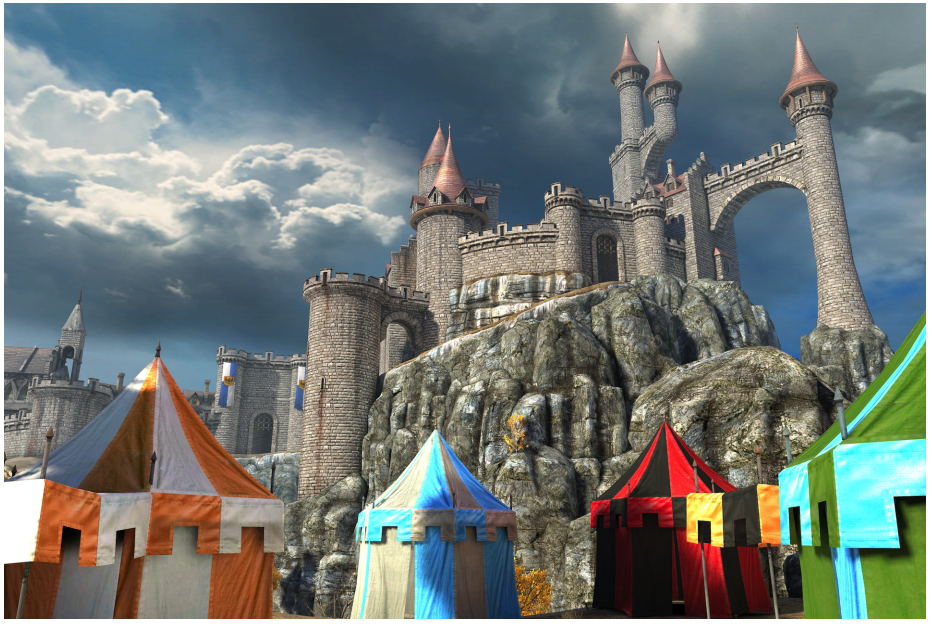
\includegraphics[width=86mm]{graphics/webGL_01.png}
\caption{Epic Games' Citadel - REFERENCE}

  \label{fig:sub1}
\end{subfigure}%
\begin{subfigure}{.5\textwidth}
  \centering
  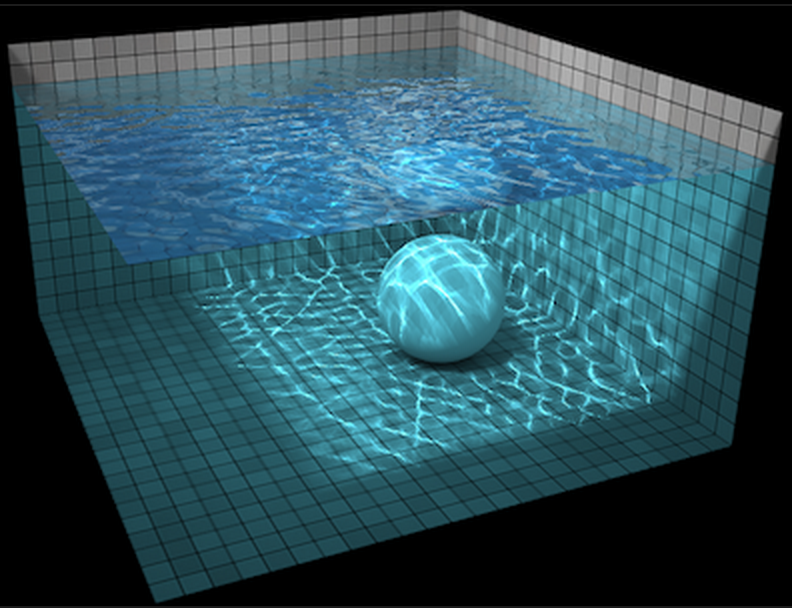
\includegraphics[width=74mm]{graphics/webGL_02.png}
	\caption{WebGL Water - REFERENCE}

  \label{fig:sub2}
\end{subfigure}


\end{figure}


WebGL is exclusively controlled by JavaScript. WebGL is based on OpenGL ES 2.0, the Embedded Systems version of the widely used OpenGL standard for generating 3D graphics. The Embedded Systems off-shoot is intended for smaller computing devices such as smart phones and tablets, such as IPhone, IPad and Android phones. Due to its smaller footprint, it was felt that WebGL would make it a more consistent, cross-platform and cross-browser 3D API (REFERENCE). 

WebGL uses the HTML5 Canvas element to render into, and uses a specific webGL-compliant context (as opposed to the 2D context used for 2D drawing). It differs in 2D Drawing, that all rendering is done with primitives such as Triangles, Points or Lines. 
Dedicated arrays called buffers are used to store the data for these primitives, such as vertices and normals. Next, a ModelView matrix needs to be created, which sets the transformation of a primitive or object in the 3D World. Also, a projection matrix is needed which converts 3D points into 2D coordinates of the drawing screen. Finally, a shader needs to be defined which will be attached to the primitives. Shaders are written in their own language called GLSL, and are themselves typically comprised of vertex shaders and fragments shaders. Vertex shaders combine the matrices and position of primitives into the final position on screen whereas the fragment shader is used to assign attributes such as color, texture and lighting. Thus, the workflow to render something with WebGL onto a webpage is as follows (Taken from book, reference):

\begin{enumerate}
\item Create a Canvas element.
\item Obtain a drawing context for the canvas.
\item Initialize the viewport, synonymous with with setting the rectangular bounds of where to draw.
\item Create one or more matrices to define the transformation from vertex buffers to screen space.
\item Create one or more shaders to implement the drawing algorithm.
\item Initialize the shaders with parameters.
\item Draw.
\end{enumerate}


As can be guessed from the steps above, WebGL is a very low level API in that it does not provide any high level scene descriptions of scene graphs. All this has to be implemented by developers manually. A large part of its draw and power stem from this fact, but also makes it very time intensive to work with from the ground up. For this purpose, some solutions already exist that build on this to provide a more convenient interface into the 3D capabilities such as ThreeJS. For this project, the XTK library plays the same role in that the low level features of WebGL can be accessed by a high-level API which can load a volume file as 3-plane slice display in a 3D View.

Nowadays, most browser-based 3D graphics libraries make use of \textit{WebGL} and even libraries that used to require a plug-in (example) have now been ported to use \textit{WebGL}. 



\newpage


\section{Implementation}

\subsection{Implemented Features}

At the end of the project, the software has been deployed to this website:

\noindent
\\
\url{http://www.davidbasalla3d.com/MscComputerScience/IndividualProject/Code/index.html}

\noindent
\\
and it has the following features:



\begin{itemize}
\item Display Layer Management

  \begin{itemize}
  \item Creation/Deletion of Display Layers
  \item Loading Medical Image Data File per Display Layer
  \end{itemize}

\item Loading of NII Volume Files (one per Display Layer), including load error management	
\item Changing of Brightness
\item Changing Image Threshold
\item Changing indices of NII Volume File
\item Viewing of NII Volume File through four bespoke cameras (X, Y, Z and 3D)
\item Custom Layouts of the four different cameras
\item Ability to pan/zoom and rotate the NII Volume File through the cameras
  item Ability to traverse by left-click and drag on a 2D-Renderer will update the other 2D Renderers to the current indices
\item Refocus the cameras by pressing 'F'
\item Two buffers to hold different Display Layers
\item Buffer Opacity and Buffer Swiping to compare the two Display Layers
\item Changing the color lookup table for a Display Layer, currently three supported Lookups (None, ID's and Heatmap)
\item Toggle for Volumetric Rendering of the Data in 3D Camera View
\item Interactive Annotation Management

  \begin{itemize}
  \item Creation/Deletion of Annotation(s)
  \item Support for multiple Annotations
  \item Customisation of Label, Color and Position of Annotation
  \item Saving out of Annotations as JSON file (via file download)
  \item Loading and Importing of Annotation JSON files
  \item Setting visibility of Annotations
  \end{itemize}

\item Labelmap Management

  \begin{itemize}
  \item Loading of Labelmaps
  \item Changing opacity of Labelmap
  \item Changing color lookup of Labelmap
  \end{itemize}

\item 'Cine' Mode for playing through Slices in a Camera View

\end{itemize}


\subsection{Layout and Input Breakdowns}

\subsubsection{Main Page Layout}



The main view that the user first sees is split into four different components. The Navigation Bar (in blue colour) contains the links to other sites such as Tutorials, Sample Data and the About webpage. It also contains the Layout Selector buttons where the user can chose a layout for the View Panels. The Display Layer Panel allows for managing of Display Layers, which are synonimous with loaded Volume files. Each Display can load a Volume File. The Levels panel contains various controls for affecting the currently selected Display Layer and its inherent Volume File. Finally the Viewer Panel contains the four different Camera View Panels that each Volume is display in. They are the perspective 3D View, and the orthogonal X, Y and Z views.

\begin{figure}[ht!]
\centering
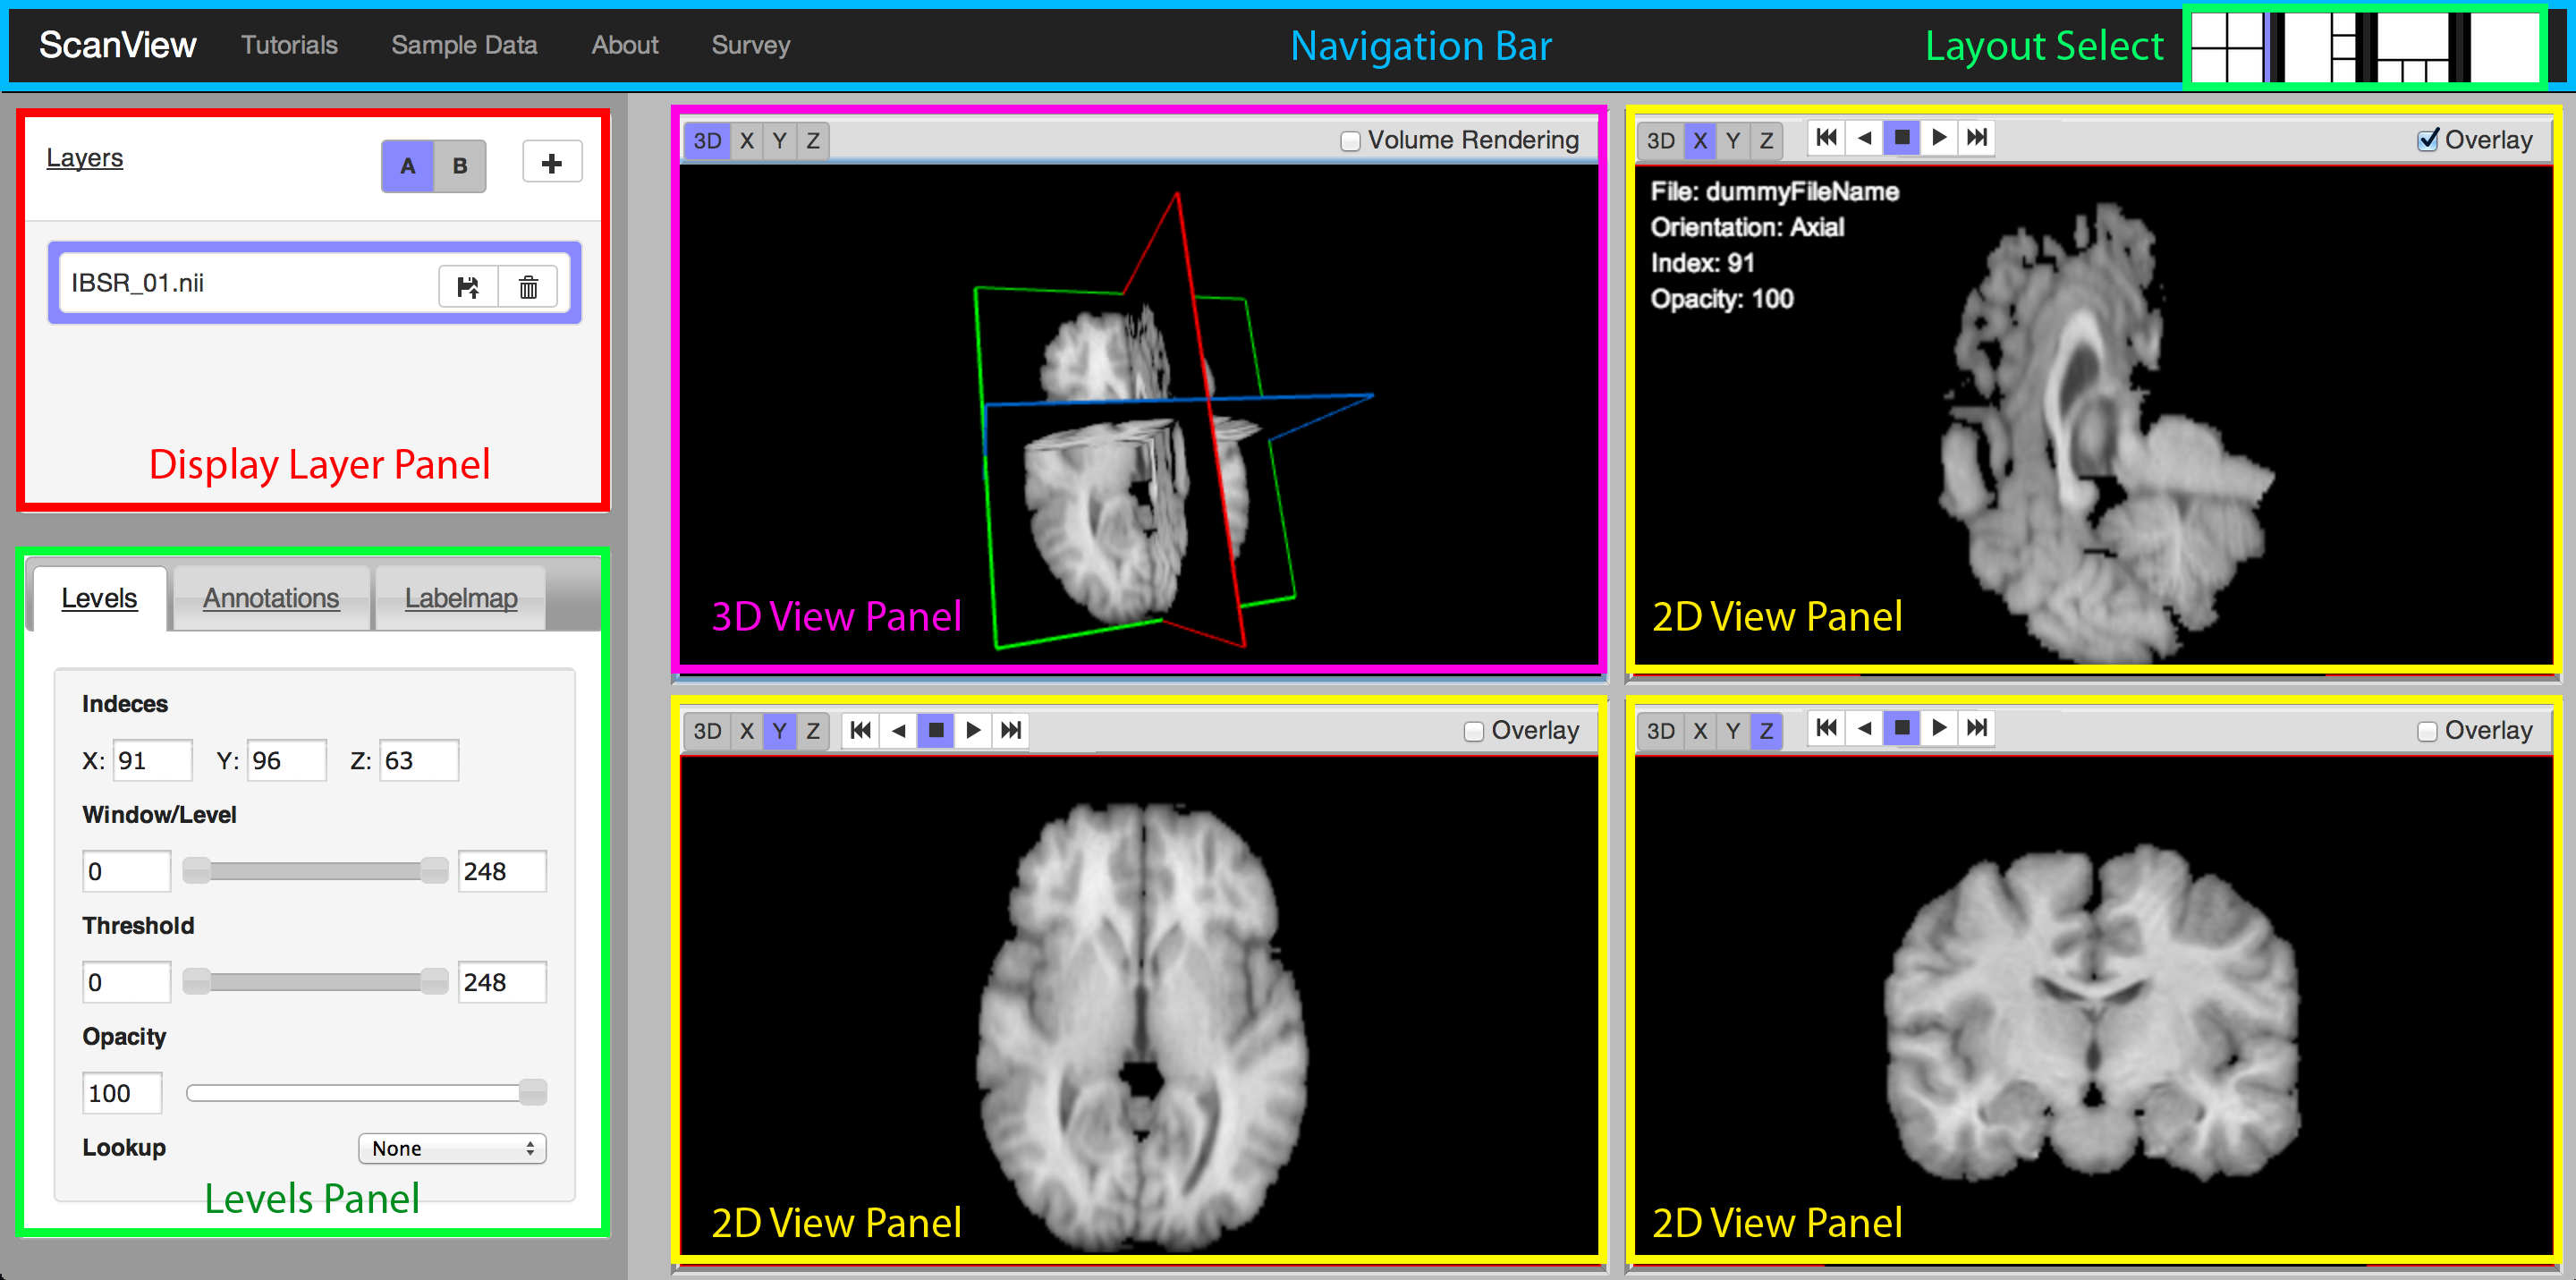
\includegraphics[width=170mm]{graphics/features_01.png}
\caption{General Panel Breakdown}
\label{fig:UIdesign1}
\end{figure}

\begin{figure}[ht!]
\centering
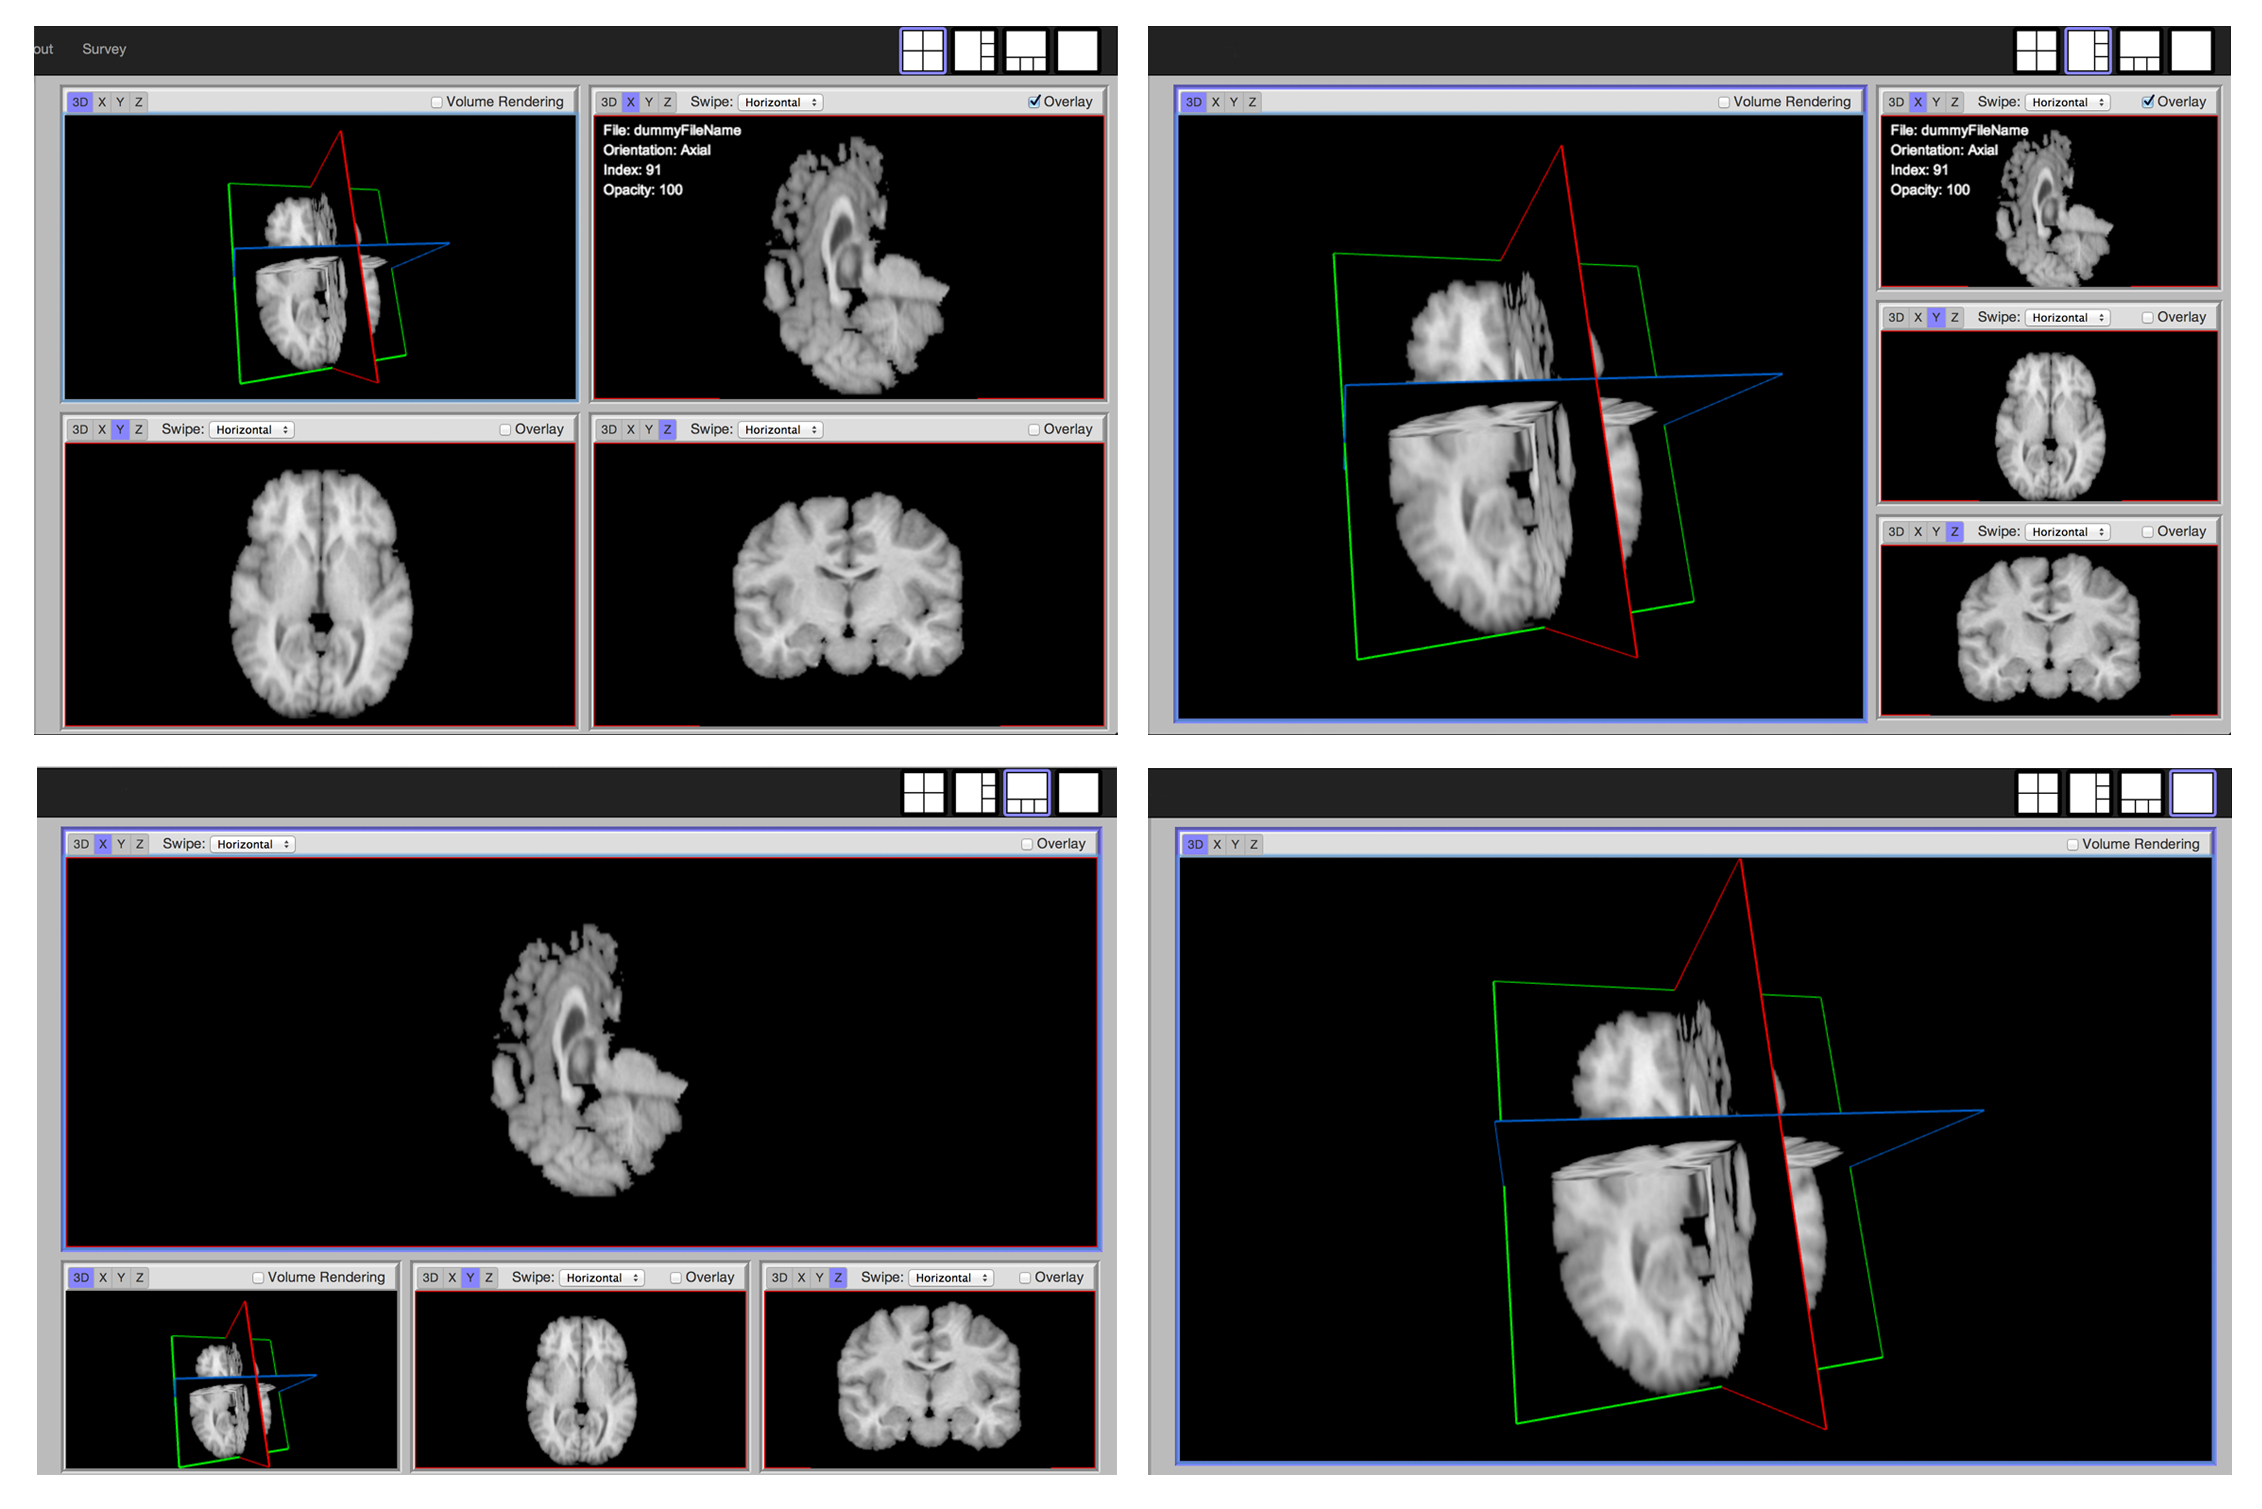
\includegraphics[width=170mm]{graphics/layouts_01.png}
\caption{Four Different Layout Options}
\label{fig:UIdesign1}
\end{figure}


\subsubsection{Camera View Panels}

\begin{figure}
\centering
\begin{subfigure}{.5\textwidth}
  \centering
  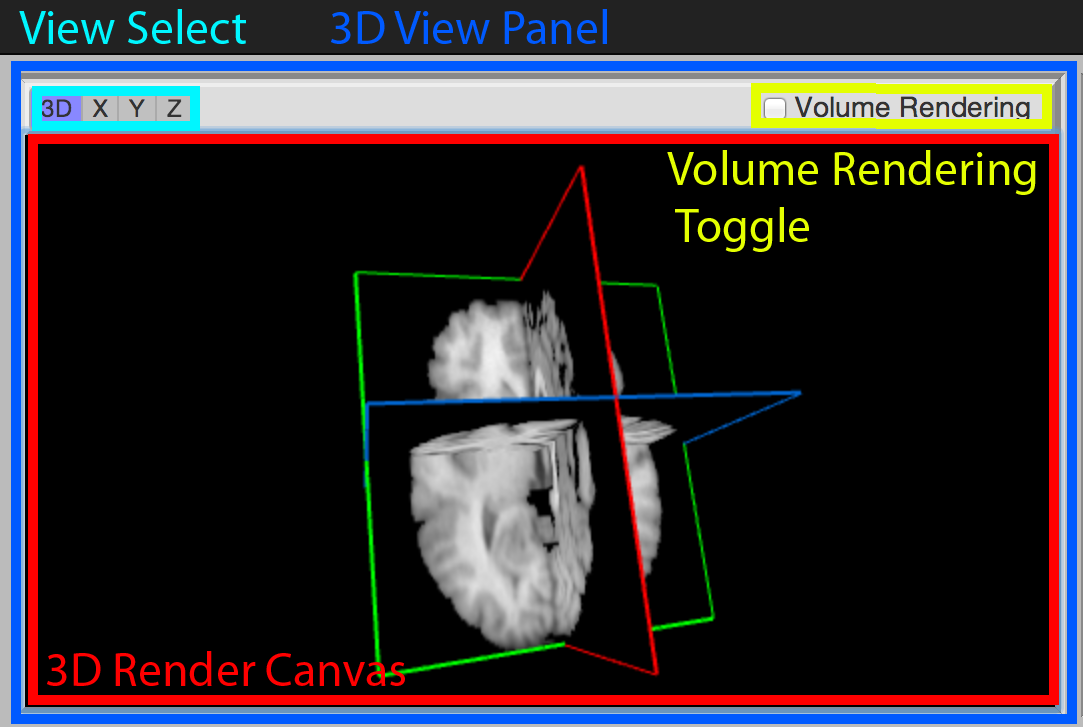
\includegraphics[width=82mm]{graphics/features_02b.png}
  \caption{3D View Panel Functionality}
  \label{fig:sub1}
\end{subfigure}%
\begin{subfigure}{.5\textwidth}
  \centering
  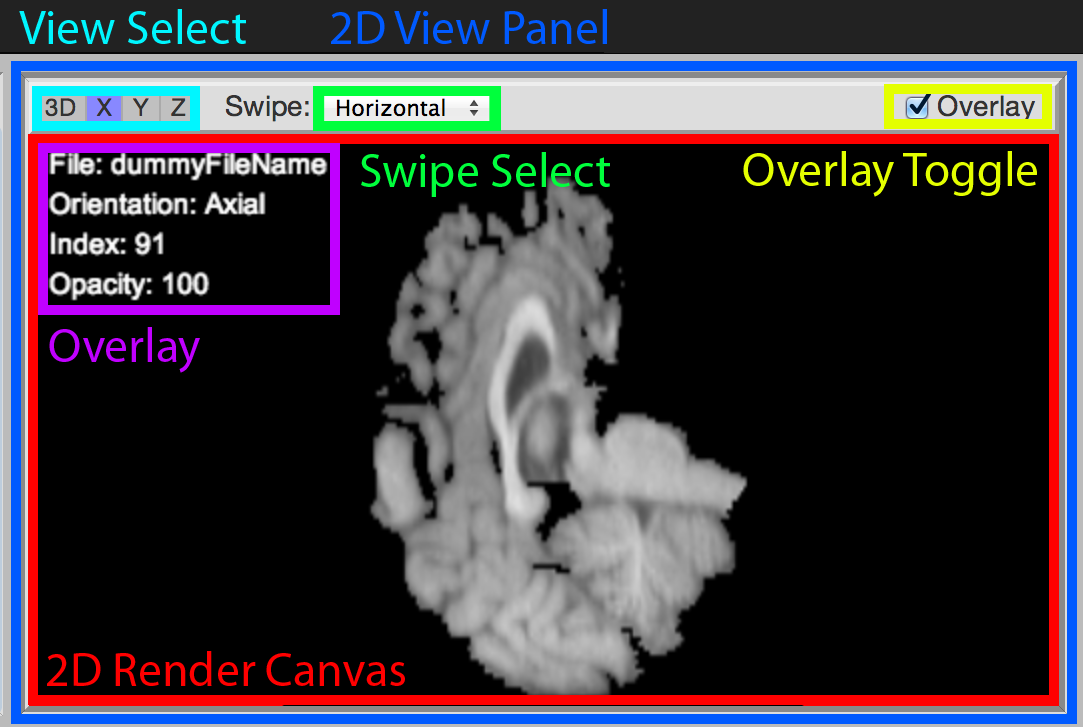
\includegraphics[width=82mm]{graphics/features_02.png}
  \caption{2D View Panel Functionality}
  \label{fig:sub2}
\end{subfigure}
\end{figure}

The Camera View Panels are the viewing windows for displaying the visual representation of the loaded Volume File. Internally they copy pixels from invisible XTK Render Panels. The View Panels hold a top bar with options to customise the viewer (e.g to specify which camera to look through). The View Panels also contain an HTML5 Canvas Element which does the drawing of the Volume File. The View Panels come in two types. The 3D View Panel displays the 3D volume with the 3 axial slices. There is an option to toggle Volume Rendering on, a feature of the XTK library. It uses WebGL and will only work on computers that support WebGL. The 2D View Panels render the orthographic (ie. axial, sagittal and coronal) views of the Volume File. They include an option to specify which way Swiping between Buffers takes place. Furthermore they have a toggle for Overlaying Information into the Viewer about current filename, orientation, index and opacity.




\subsubsection{Display Layer Panel}

\begin{figure}[ht!]
\centering
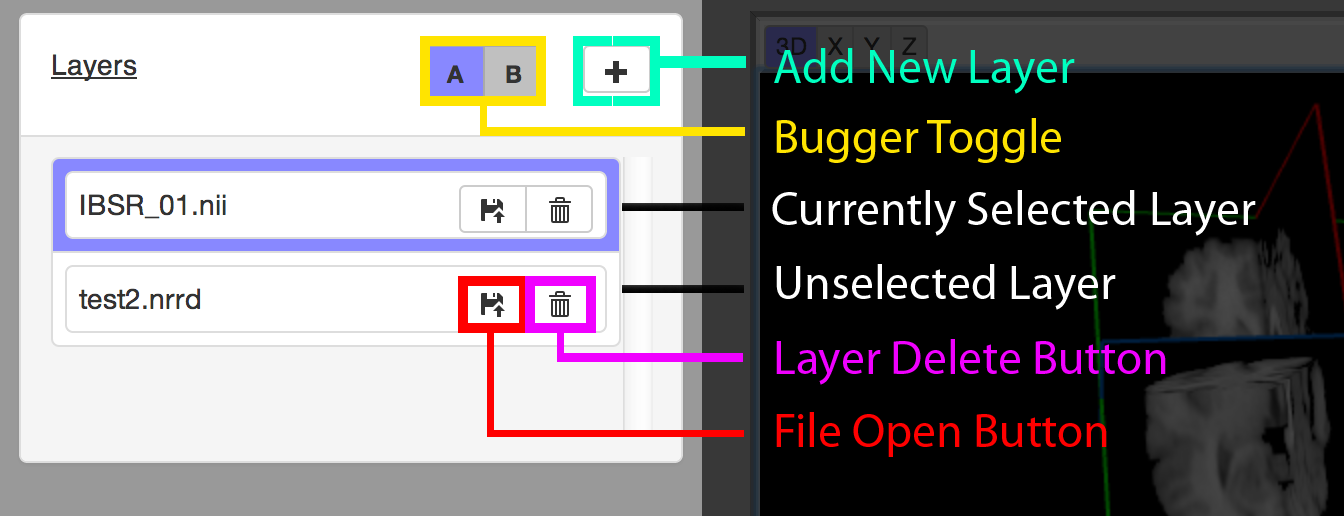
\includegraphics[width=140mm]{graphics/features_03.png}
\caption{Display Layer Panel Functionality}
\label{fig:UIdesign1}
\end{figure}

The Display Layer Panel allows the user to manage Display Layers by creating, deleting and modifying them. Each Display Layer can load a Volume File, which will be displayed in the View Panels. Multiple Layers can be created and will highlight blue when selected. Additionally there is a Buffer Toggle Button which allows to switch the viewer between Buffer A and Buffer B. Each Buffer can hold a different Display Layer. This becomes useful when adjusting the Opacity of a Display Layer and it will reveal the Display Layer in the B Buffer. When Buffer A and Buffer B hold the same Display Layer, dialling down the opacity will fade the View Panels to black. Also the Buffer Swipe feature (hold Ctrl and move mouse over a 2D View Panel) plays into this.

\begin{figure}
\centering
\begin{subfigure}{.5\textwidth}
  \centering
  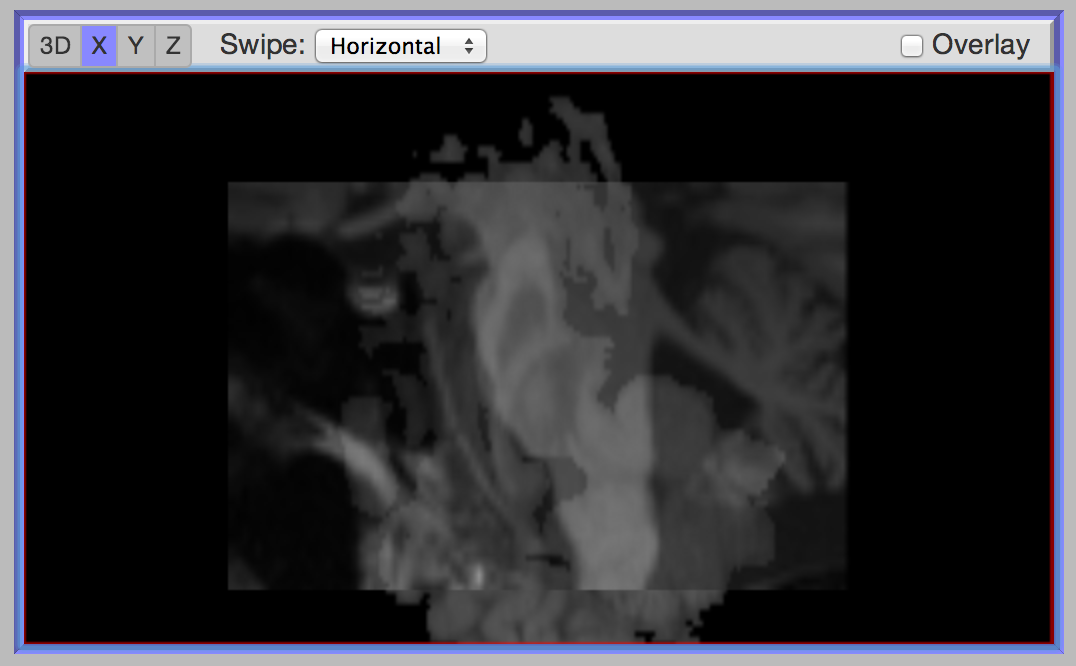
\includegraphics[width=82mm]{graphics/BufferOpacity_01.png}
  \caption{50\% Opacity on Buffer A with revealed Buffer B}
\end{subfigure}%
\begin{subfigure}{.5\textwidth}
  \centering
  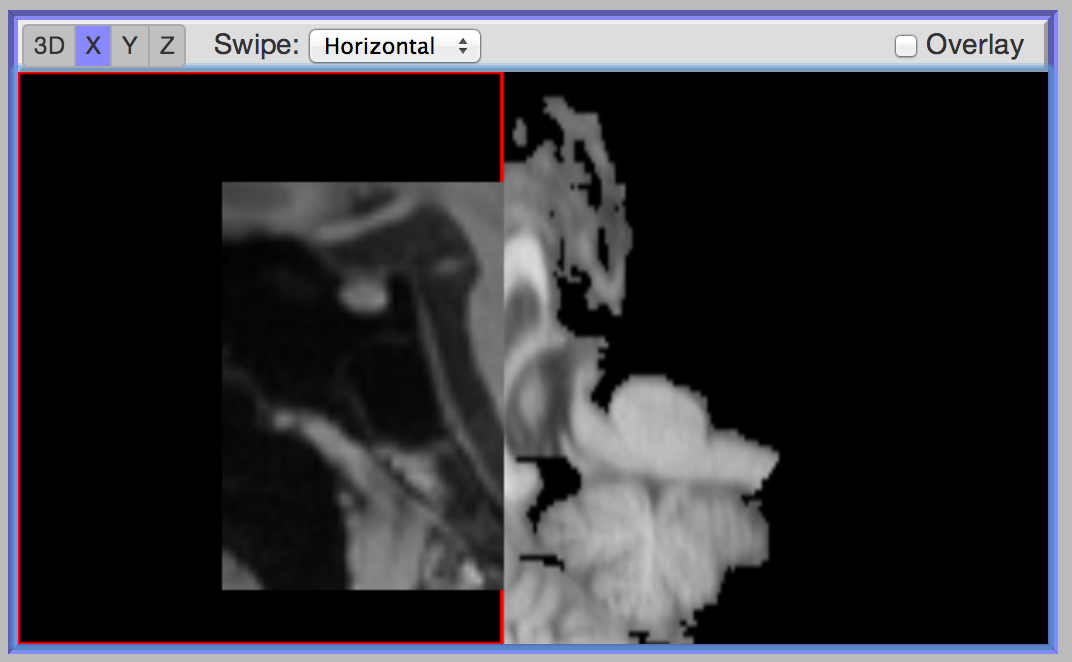
\includegraphics[width=82mm]{graphics/Swipe_01.png}
  \caption{Horizontal swiping between two different Buffers}
\end{subfigure}
\end{figure}




In terms of mouse and keyboard input controls, the 3D Render Canvas supports the common operations of panning, zooming and rotating via mouse controls. Pressing 'F' on the keyboard will reset the camera to the initial setting. Pressing 'v' will toggle the Volume Rendering toggle. Likewise for the 2D Render Canvases, panning and zooming are supported, as well as 'traversing'. When the user clicks the left mouse button and floats the mouse across the slice rendering, the indices will update in the other viewers accordingly as to where the mouse pointer is in the selected View Panel. Also, pressing 'f' will reset the camera. Pressing 'o' will toggle the Overlay toggle.




\subsubsection{Levels Panel and Tab}

\begin{figure}[ht!]
\centering
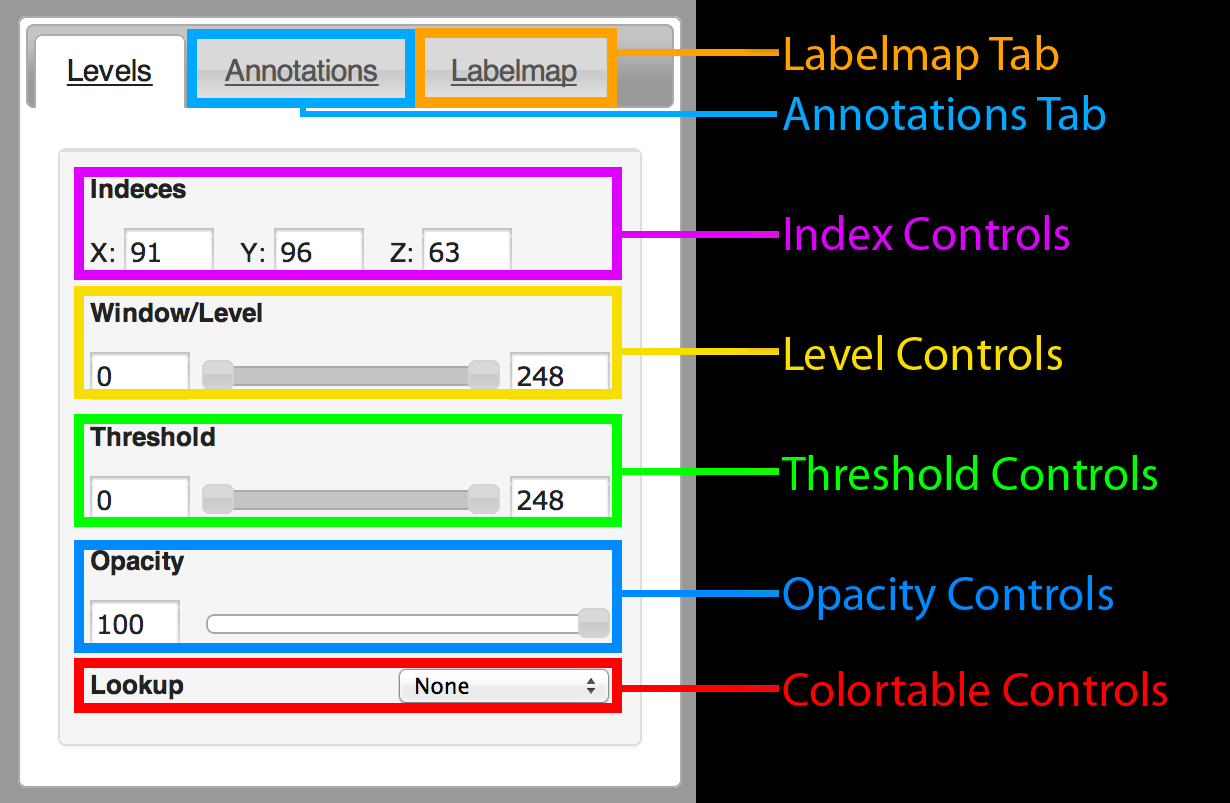
\includegraphics[width=140mm]{graphics/features_04.png}
\caption{Levels Tab Functionality}
\label{fig:UIdesign1}
\end{figure}

The Levels Panel contains separate tabs that enable further customisation of the currently selected Display Layer. In the Levels tab, a number of convenient controls are provided. Firstly, the Index Controls provide feedback on which Slice Indices are currently set. These can also be altered via the number input. 

Next, the Window Controls can be used to control the Brightness of the loaded Volume File. This attributes straight into windowLow and windowHigh attributes of an X.volume. Likewise, the Threshold Controls allow for a clipping of a Volume File and is also provided by default by the XTK library.

The Opacity Controls allow the user to set the opacity of the currently loaded Display Layer. Depending on what is loaded in the other Buffer, this will either reveal the Volume File from other Display Layer or fade to black.

Finally, the Colortable Controls allow for switching the Colortable to one of three options (None, IDs and Heatmap). This changes the color value lookup at render time, making the Volume File look different with each option. IDs is generally intended for use with Labelmaps, whereas Heatmap can be used for any Volume File.



\subsubsection{Annotations Tab}

\begin{figure}[ht!]
\centering
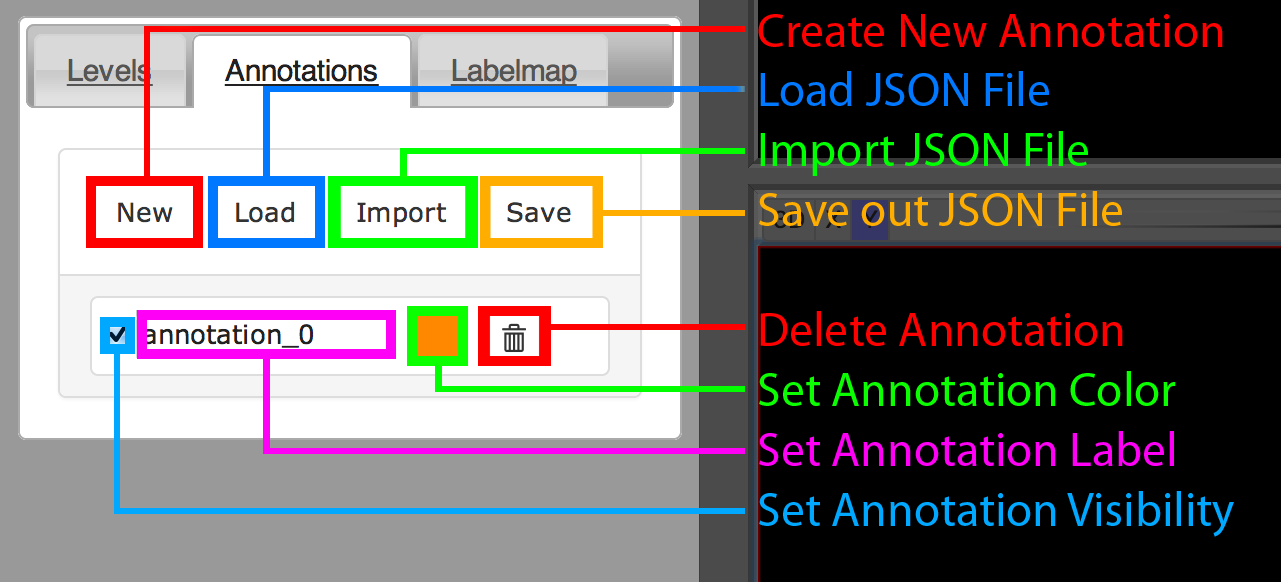
\includegraphics[width=140mm]{graphics/features_05.png}
\caption{Annotation Tab Functionality}
\label{fig:UIdesign1}
\end{figure}

The Annotations Tab allows the user to create, load, customise and delete Annotation Layers. When the user hits 'New', a new Annotation Layer is created, based at the current Volume File indices position with a prespecified width, length and breadth. The user can then toggle the visibility, change the label and color. Clicking on the color button will open a Colopicker UI. Finally each Annotation Layer has a Delete Button. Multiple Annotation Layers can be created. The UI allows for loading (via 'Load') a JSON file which will remove all current Annotation Layers and create the Layers as specified in the JSON file. Clicking 'Import' will add Annotations from a JSON file to the current Annotations. Lastly, clicking the 'Save' Button downloads the current Annotations in JSON format to the users computer. This would otherwise cause a 'Save As'-style UI modal screen to pop up, but Web Browser do not supply this feature for security reasons.



\begin{figure}[ht!]
\centering
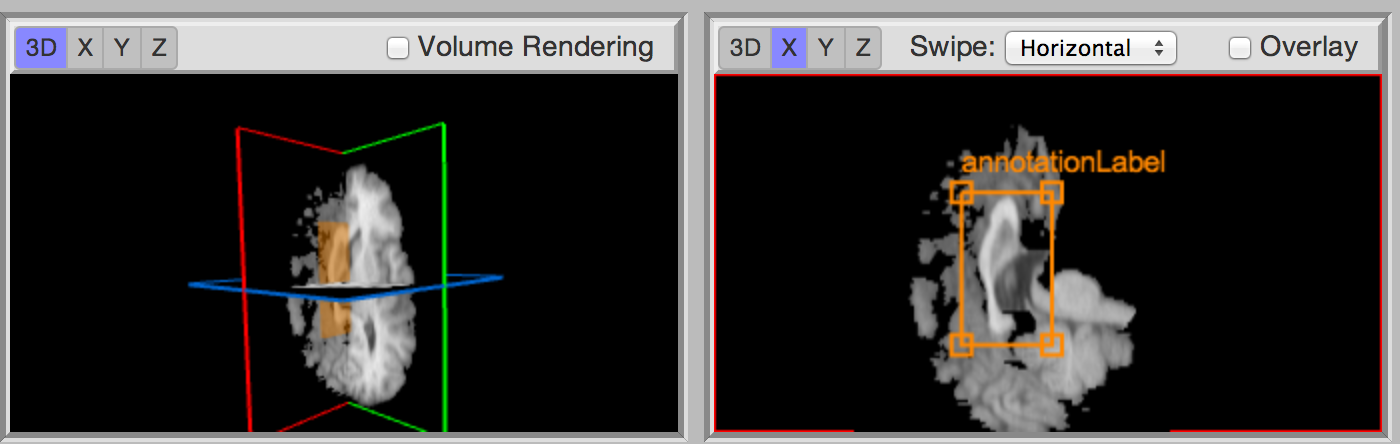
\includegraphics[width=170mm]{graphics/AnnotationFinal_01.png}
\caption{Annotation in 3D and 2D View}
\label{fig:UIdesign1}
\end{figure}


A visible Annotation is displayed as a rectangular volume in the View Panels, colored as per the color specified in the Annotation Layer, with the Annotation label being displayed above it in the 2D Panel Views. The corner points are selectable and manipulatable in the 2D Panel Views. Moving one point will move its neighbor points accordingly to keep the rectangular shape. There is a fixed limit to how small an annotation can be made. When a Annotation point is selected, it's according layer is highlighted blue in the Annotation Tab.




\subsubsection{Labelmaps}

\begin{figure}[ht!]
\centering
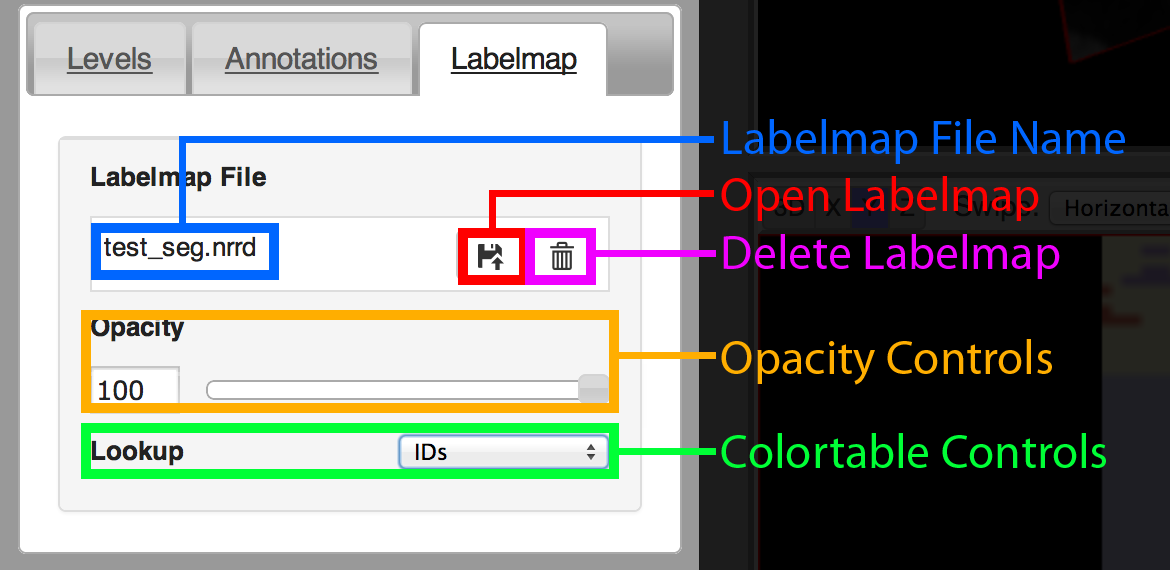
\includegraphics[width=140mm]{graphics/features_06.png}
\caption{Labelmap Tab Functionality}
\label{fig:UIdesign1}
\end{figure}

Labelsmaps can be loaded via the Labelmap tab. The UI allows the user to load one labelmap. There is a Opacity Control for setting the Labelmaps opacity and a Colortable Selector provided. The Colortable Selector provides the same three options as for the Levels tab.




\subsection{Development Strategy}

Generally the development strategy for this project was to program in modular fashion, tackle problems in a naive fashion first to test for any big problems or in other words to create prototype solutions first. Once a certain prototype milestone had been achieved, some time was spent on refactoring code based on insights learned. A Todo list was maintained throughout the project against which items were ticked off as completed when done. Regular meetings were held with the project supervisor Dr. Ben Glocker to ensure that the project was on the right track. As this was an individual project and no other programmers were involved, team organisation or communication was not an issue.

\subsubsection{Meetings with Supervisor}

Meetings with the Project Supervisor Dr. Ben Glocker were held every one to three weeks, based on availability. Written notes were kept as record. Generally we discussed my progress up to date, and which features I should focus on in future. The meetings provided valuable feedback and direction, since Dr. Glocker is an expert in the field of Medical Imaging, has written his own Medical Image Viewers and could provide relevant Software and Data samples. He was treated as the client for this project.


\subsubsection{Test Data}

My supervisor provided a host of test files for me to use while developing this tool. These varied from smaller files of a brain scan (4.2 Mb) with a labelmap (4.2 Mb), to the largest scan file of an abdomen (86.5 Mb). Additionally I downloaded some sample data from the XTK tutorials. This set included the main file (286 Kb), a labelmap (19 Kb) and a colortable (6 Kb). Furthermore I downloaded more samples from the official Nifti website. For testing new features, I would test the thorax file set, as well as the brain scans, since these files took less time to load. Periodically I would test the other Nifti files to make sure the code worked with diffferent and larger files.
For colortables, I downloaded some from the 3DSlicer wikipedia site in their default format, and later amended these to work as hardcoded\textit{JavaScript}arrays.

Dr. Glocker kindly also supplied a number of desktop programs for medical image viewing that I could use for inspiration, such as IMView and MIT3K.

\subsubsection{Coding Journal}

As the project grew more complex, I started writing a Coding Journal in which I would write down any relevant ideas or thoughts. Since working on one aspect usually took more time than thinking of ideas for other aspects, this proved quite valuable in recording them, organising them and going back over later to make sure I had not missed anything important.

\subsubsection{StackOverflow}

As I am sure is a regular occurence, checking StackOverflow for any problems proved invaluable. At time of writing, there are 15,957 questions tagged with 'Backbone', 521,973 questions tagged with 'JQuery' and 681,696 questions tagged with 'JavaScript', so it provided a vast resource for fixing problems. Even for XTK there are 139 Questions tagged, which is relatively small given the other numbers but still useful due to the occasional answer of the XTK authors themselves. Three of the questions tagged with 'xtk' have been asked by me.



\subsection{General structure}

The initial plan was to build a UI with custom features (the frontend) using the XTK library with its API calls as the backend. The hope was that the XTK library would provide all necessary functionality required and so it would not be necessary to alter the library itself. However it soon became apparent that this would not be the case.

The frontend would be written purely in\textit{JavaScript}and structured with Backbone, and be using RequireJS to handle the various dependencies. Twitter-Bootstrap and JQueryUI would be used to style the look and feel of the frontend.

The backend ie the XTK library is also written in JavaScript, but uses the Google Closure library to compile the code into minified code. This serves to reduce variable and function names and generally is designed to make the code run faster. The drawback is that it become harder to decode, since variable and function names are changed to be meaningless to the human reader. For functions and attributes that are meant to be used from outside the library, custom setters and getters have to be written. XTK also uses Goog matrices for their Graphics computations. Additionally the WebGL portion of XTK makes use of GLSL for its shaders, but is wrapped as strings in a\textit{JavaScript}file.


\subsection{Implementing Features/ Implementation History}

This subsection will deal with the implementation of general and specific features of ScanView. For clarity's sake, the reader should be aware that the XTK Library consists of several classes, and that the main rendering interface (including the Canvas element that is used for drawing) is called an X.renderer. A more detailed explanation of XTK's inner working will follow in the next section, where I discuss my experiences of the various libraries that were used on this project.


\subsubsection{Creating the single web app structure}

I started the project with one of the tutorial from the XTK website. Tutorial 13 had a very basic setup that was similar to what I intended for my project - a four panel rendering of a volume data file. The tutorial has less than 100 lines of Code, with half of it used for specifying an inbuilt GUI. Since I wanted to create a custom GUI and generally have a much bigger codebase, first I need to ensure that I had a solid structure for my project. This is where Backbone and RequireJS came into play. Since I was not entirely familiar with either of them, it took a few days to get up to speed and try out a few tutorials to familiarise myself with their useage. After a few days I had managed to create a frame work that mimicked the tutorial, but was running in the confines of Backbone with proper models, views according to the MV* pattern and managed dependencies through RequireJS. Figure ~\ref{fig:generalUML} shows a UML-style representation of the adopted architecture. 

\begin{figure}[ht!]
\centering
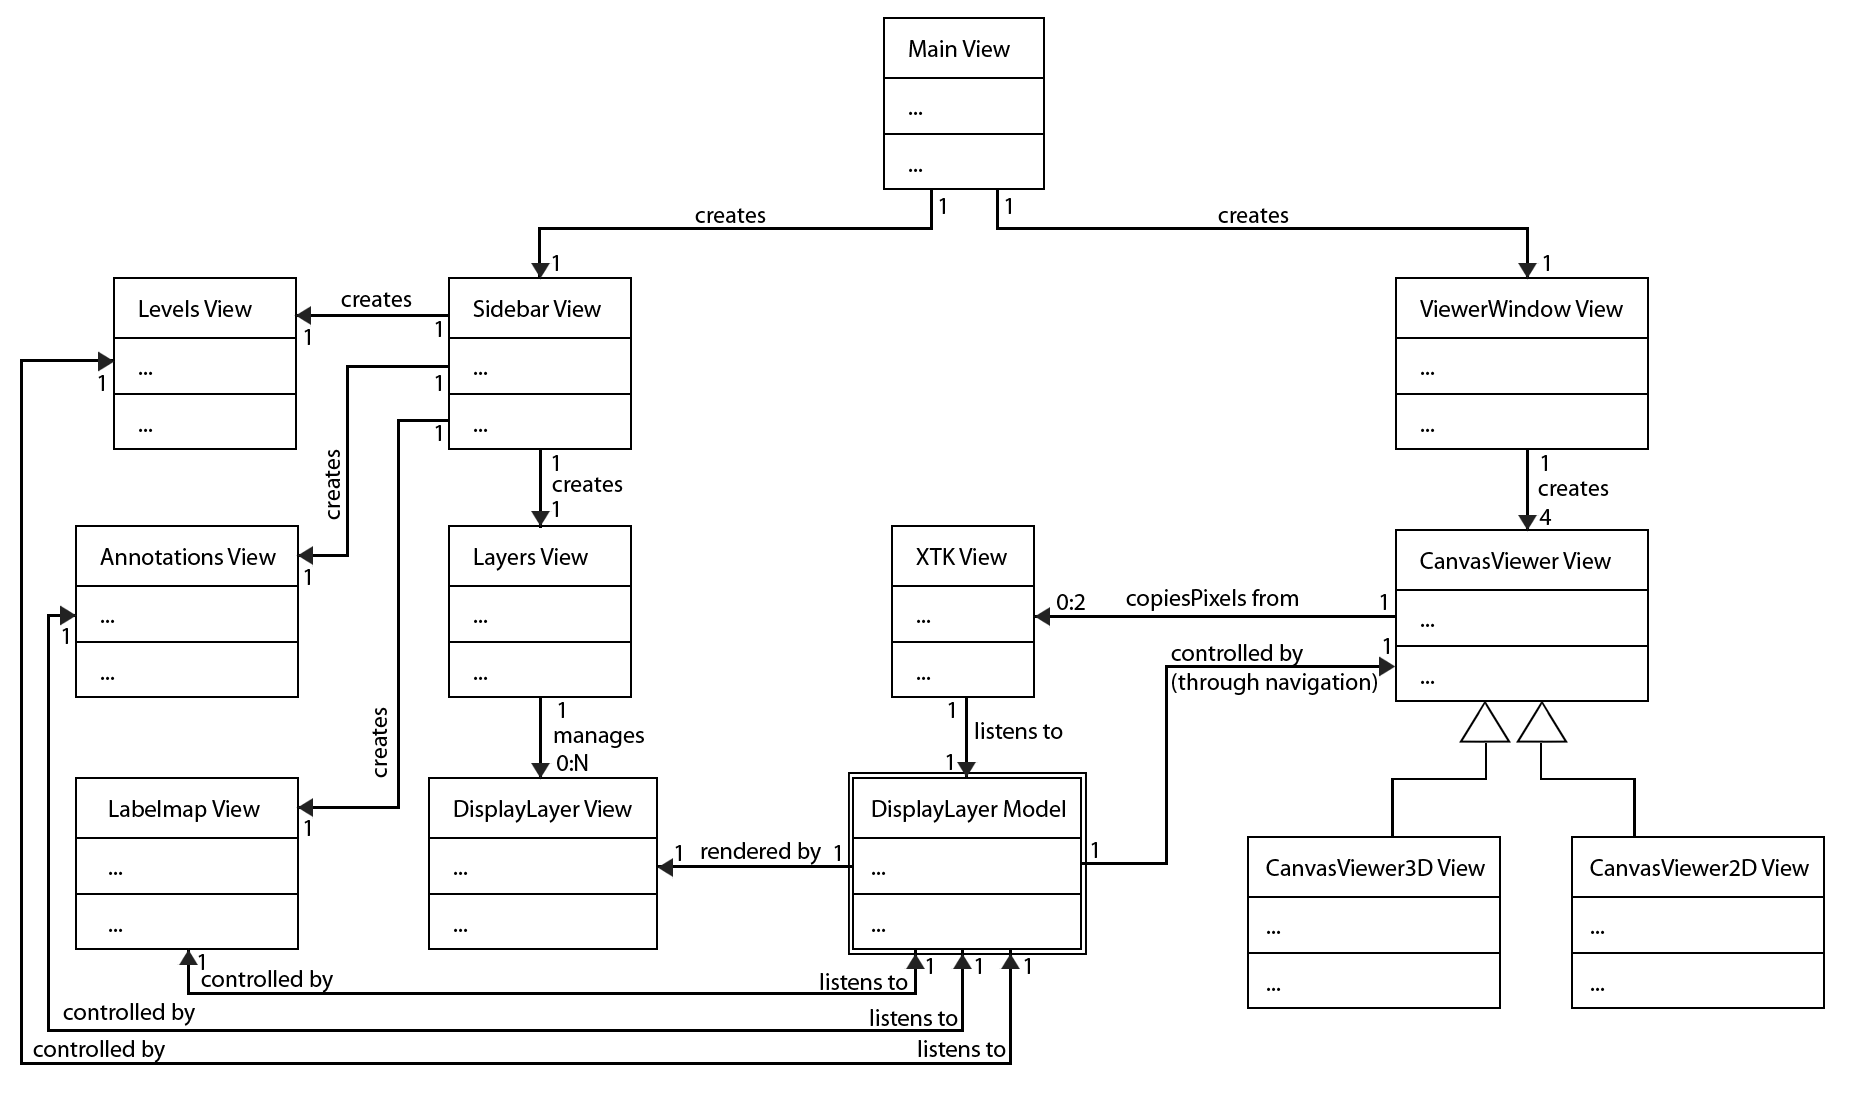
\includegraphics[width=170mm]{graphics/generalUML_v01.png}
\caption{Display Layer Model Class Diagram}
\label{fig:generalUML}
\end{figure}

The key idea is that the Display Layer is the main Backbone model and thereby central to the whole architecture. It is here that file data is stored for each volume, as well as attributes such current indices, brightness, windowing and everything else relevant for displaying a Volume File. Figure ~\ref{fig:layerUML} shows the class diagram for the Display Layer model.


\begin{figure}[ht!]
\centering
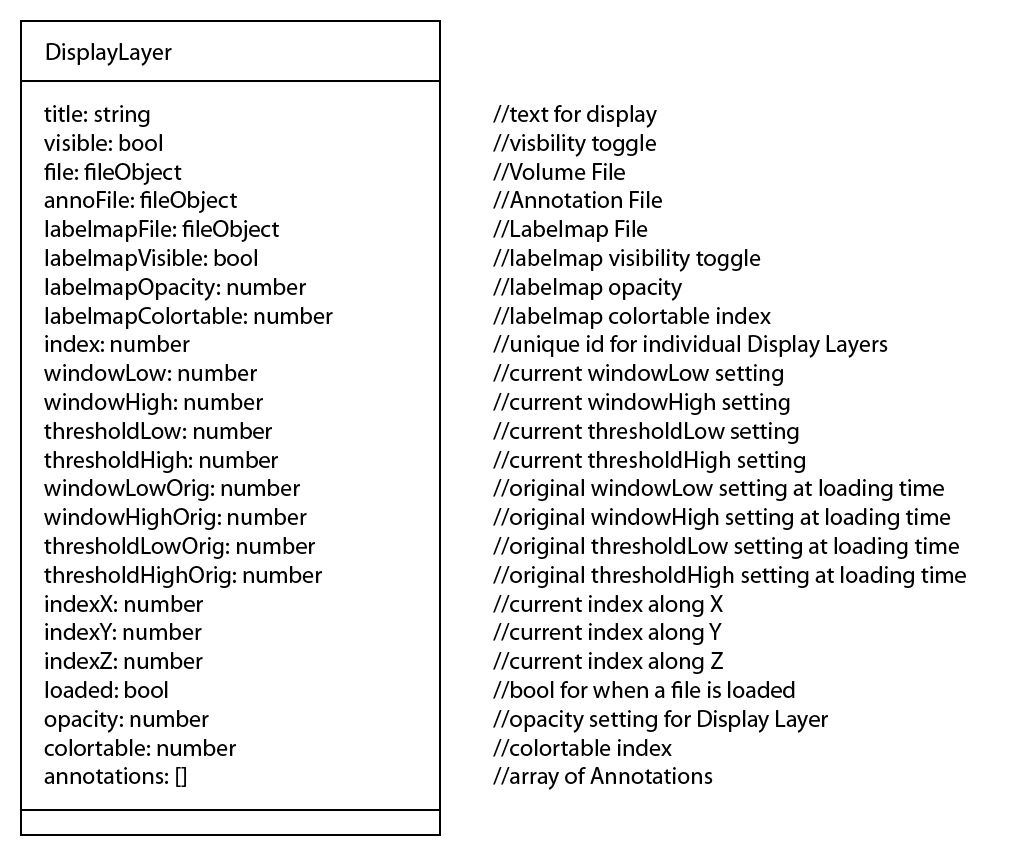
\includegraphics[width=140mm]{graphics/displayLayerUML_01.png}
\caption{Display Layer Model Class Diagram}
\label{fig:layerUML}
\end{figure}

Each Display Layer Model instance has a Display Layer view, which renders a Layer item in the Display Layer Panel. Everything else is managed by Backbone Views. These Views generally listen to the DisplayLayer Model to see if any attributes have changed. If this is the case, then the View is upated accordingly due to internal function calls. The individual Display Layer Views are managed by a Layers View (which admittedly could have been named more clearly), which handles Layer Creation, Deletion and Ordering. The specific settings for a Layer, as displayed in the Levels, Annotations and Labelmap tabs are also separate views. Due to the nature of Backbone's Views taking on the role of MVC Controller as well, these Views listen to events from the Model, but can also set attributes of the model directly, as illustrated in the diagram.

For rendering, there exists a main ViewerWindow View which controls functionality for the four DisplayPanels. Each DisplayPanel is also its own View. In fact, these have an abstract parent View called CanvasViewer, which CanvasViewer2D and CanvasViewer3D inherit from. Importantly, there is an XTK View, which contains the actual X.renderers. All interaction of the frontend with the XTK library backend happened exclusively through this View. An instance of this view is created for each DisplayLayer Model. These Views listen to the DisplayLayer Model and update the contained X.renderers accordingly. These XTK Views are hidden from the user, but their canvas' pixel values are copied by the CanvasViewer Views. When a new Display Layer is selected, the CanvasViewers stop copying the old XTK View's canvas and instead copy from XTK View linked to the new Display Layer. Again, the fact that Views also act as Controllers, means that user interaction with the CanvasViewer View (such as scrolling to set a new slice index) can directly set attributes in the model.


The decision to have the CanvasViewers Views copy the pixel data from the XTK Views was important, in that it allowed more customisation of the main View Panels. The image data from the XTK Views were essentially one image buffer. I could now add additional buffers as required. For example I added the Overlay feature, which display some info text (like current Slice index and filename) in the Canvas. Also the opacity feature and Buffer swiping (which will be discussed later) were easier to implement. Technically, the copying is done with Canvas' drawImageData() function at the requestAnimationFrame function. DrawImageData() allows for drawing on a Canvas the contents of an image file or another Canvas elements (the canvas of the XTK renderers in this case). The requestAnimationFrame function is new with HTML5 and is intended the use of setTimeout() which was traditionally used to trigger at specific interval time. It basically aims to deliver the best performance given the current CPU load and monitor refresh rate (REFERENCE).


The XTK View in itself contains of four X.renderers (3D, X, Y and Z). Initially I was planning to separate each X.renderer into a separate XTK View. However, due to XTK implementation, there exist some dependencies between these X.renderers, in that one X.renderer is a designated first viewer which takes care of all the file loading and parsing. When this is done, a signal called 'onShowtime' is emitted. This is the cue for other renderers to start rendering their newly loaded content, without having to load anything again. Due to this interplay between the renderers, I decided to bundle all of them into one View, and let all access to the X.renderers be handled by the XTK View.

Finally there is a MainView which creates a Sidebar View and the ViewerWindow View. The Sidebar View create the DisplayLayers View as well as the Levels, Annotations and Labelmap Views.


\subsubsection{Loading Volume Files}

After creating the initial structure, tackling the issue of loading local volume files was the next step. This can be tricky with Web Browsers, as for security reasons file I/O is not a feature that is readily supported. However I had the SliceDrop code to look through. This was all implemented in the XTKView, and basically copying the data into a local container did the trick. This is done with the HTML5 FileReader element, which allows for asynchronous file loading in various formats (text/buffer, etc). The FileReader loads a file asychronously and emits a signal when it has finished. The resulting fileObject could then passed onto the XTK renderer to load and parse the file.

Once I had this setup I came across one of the first bugs in XTK. When loading NRRD files, the volume would load and display, but it would be slightly offset. Testing this on a couple of Desktop solutions which worked fine let to the conclusion that it is a bug in the XTK library. 


\subsubsection{View Panel Layout}

In terms of the layout of the components of ScanView, it needed to accomodate the four different views (one 3D Camera View and X, Y and Z Camera Views). I wanted to add some customisation options in terms of size of the viewer and choice of Camera View in each panel. Depending on whether it was a 3D or 2D Camera View, the Display Panel would have different options. 3D Camera View needed a toggle for Volumetric Rendering, 2D Camera View needed a toggle for Information Overlay.

For the different layouts I briefly investigated using interactive splitters, but found them to be not very easy or reliable to tie into the program. Instead I opted for 4 different static Layouts (See image below). This should give the user enough options to choose what his prefered layout. Implementing the logic behind these panels took a while to get right. Panels had to auto-resize everytime the layout was changed. Again this required some exposing of extra XTK attributes, as well as CSS management of the CanvasViewer Views.

Implementing the feature to change the current viewer orientation took a little bit of time to figure out. I experimented first with a fixed order of CanvasViewers (meaning their order in the DOM), where changing a CanvasViewer's orientation would cause its Canvas element to start copying a different XTK Viewer. This proved to be cumbersome to manage, as not only the Canvas content but also the buttons of the CanvasViewer had to change (e.g 'Overlay' or 'Volume Rendering' toggle) depending on if the 3D camera view or the orthogonal views were selected. Instead I opted for a floating order of CanvasViewers, so that depending on selection, the CanvasViewer would be reordered in the DOM to appear at the correct position. This meant that the CanvasViewer View itself stayed intact with all functionality, only its position and possible size had changed.


\subsubsection{Buffer Management}

As the next step, I introduced Buffers. Conceptually, this was taken from the Image Compositing Software Nuke, discussed in the Desktop Software section, where the user can store different Display Layers in the Buffers. This involved some deliberate thought, as the interplay between the buffers would determine the rendering on them in the CanvasViewer Views (with opacity and swiping). I created a separate Backbone Model to keep track of which Display Layers were stored in which Buffer. I then changed the code of the CanvasViewer Views, so that they always store a background and a foreground DisplayLayer. The CanvasViewer View listens to the Buffer Model to determine which Display Layer will be in the forefround, and which in the background. This comes down to the stored Display Layers and the currently selected Buffer. 

With the above in place, I could easily implement opacity blending and buffer swiping, since I had access to both Display Layers in my CanvasViewers. I changed to code for the CanvasViewer draw() to draw first the background Display Layer's content and then the foreground Display Layer's content on top of it (only if the opacity of the foreground was less than 100\%). For drawing to Canvas with opacity, I made use of Canvas' inbuilt globalAlpha attribute. So when using the drawImageData(), it would only draw it with the specified opacity of the globalAlpha attribute, thereby revealing the content of the background layer. For buffer swiping, a similar approach was used. Again, the background is being drawn fully, and the foreground is only drawn within a specific region as controlled by the user. This was easily done, as the drawImageData() function takes Canvas coordinates as input of where to draw to. 




\subsubsection{Colortables}

The next feature I tackled was Colortables, with which to change the color output for a given volume. The XTL library does support Colortables, which ironically ended up costing me a week of coding time. XTK Colortables follow the same format as 3DSlicer's format and a Wikipedia site with which one can create custom Colortables exists online. The format is that each line is prefixed by an index, which will usually by the RGB value of the volume data. Each line is then mapped to a label and a set of RGBA values.

\begin{figure}[ht!]
\centering
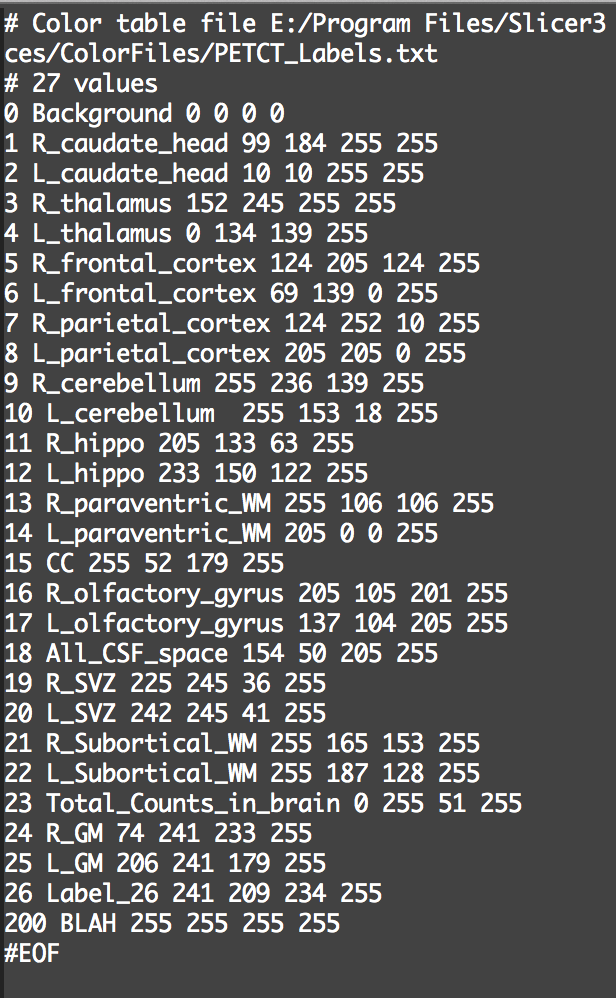
\includegraphics[width=70mm]{graphics/Colortable_01.png}
\caption{Example of a Colortable}
\label{fig:UIdesign1}
\end{figure}

XTK deals with Colortables in that the user has to load them as a .txt file when adding the Volume data and other input files. Thereby it is bundled up with the rest of the IO processes. Again, as with normal file loading, XTK is not designed for adding or modifying these kinds of files at runtime, so I had to add this functionality. This took a long time in that I had to trace the whole function flow of XTK when loading files. I proceeded with various steps, but would encounter problems at every stage, since I was forcing XTK do something that was not really inherent in its initial design. At a very basic level, colored displays (ie varying R, G and B channels) were not enabled for volumes by default, so I had to edit the code for that. On top of that, 2Drenderer and 3DRenderer deal with color and rendering quite differently. The 2D renderer does the rendering to screen space at a specific time per second. The 3D renderer uses a fragment shader (like in OpenGL) to assign color. Figuring all this out took a while, and after 7 days I had finally managed to get the whole process working. The only problem was that since I/O was involved, it would take quite a bit of time to update, so it was not entirely slick. Also, the way XTK loaded these colortables was by actually baking the colors into the slice texture. 




\begin{figure}
\centering
\begin{subfigure}{.33\textwidth}
  \centering
  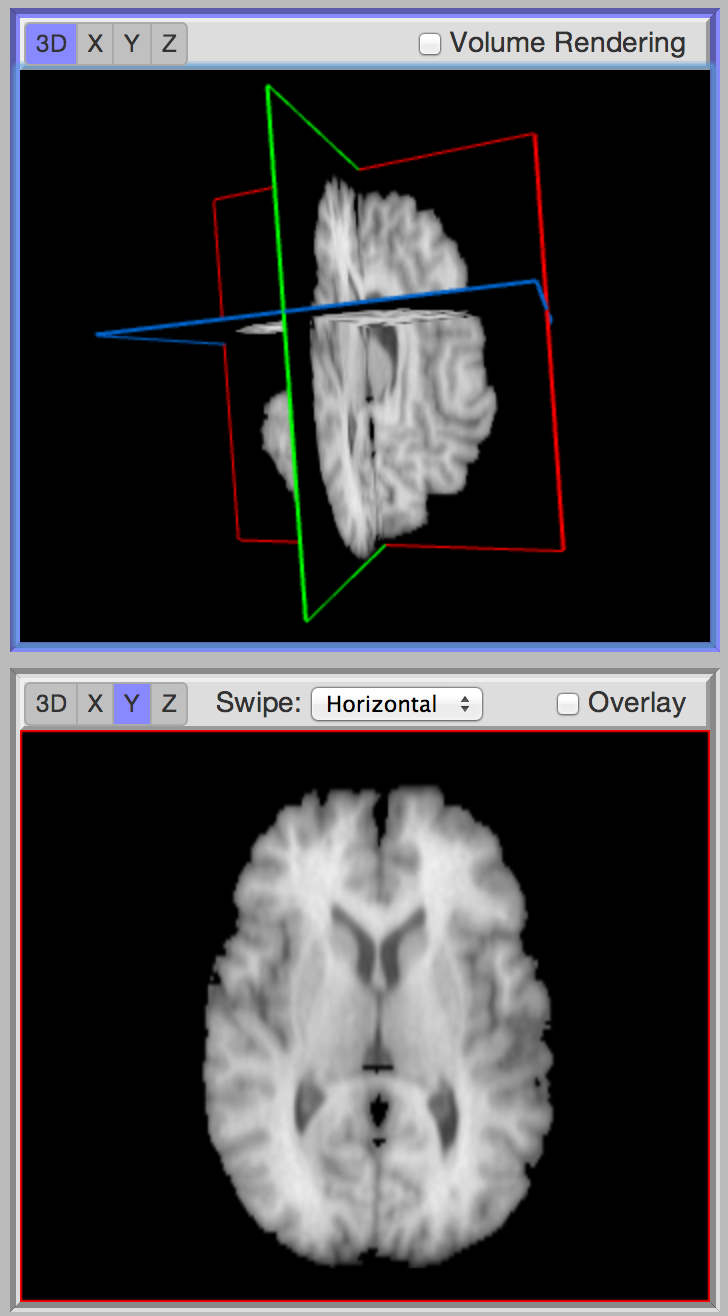
\includegraphics[width=52mm]{graphics/ColortableB_02.png}
  \caption{Colortable Option 'None'}
\end{subfigure}%
\begin{subfigure}{.33\textwidth}
  \centering
  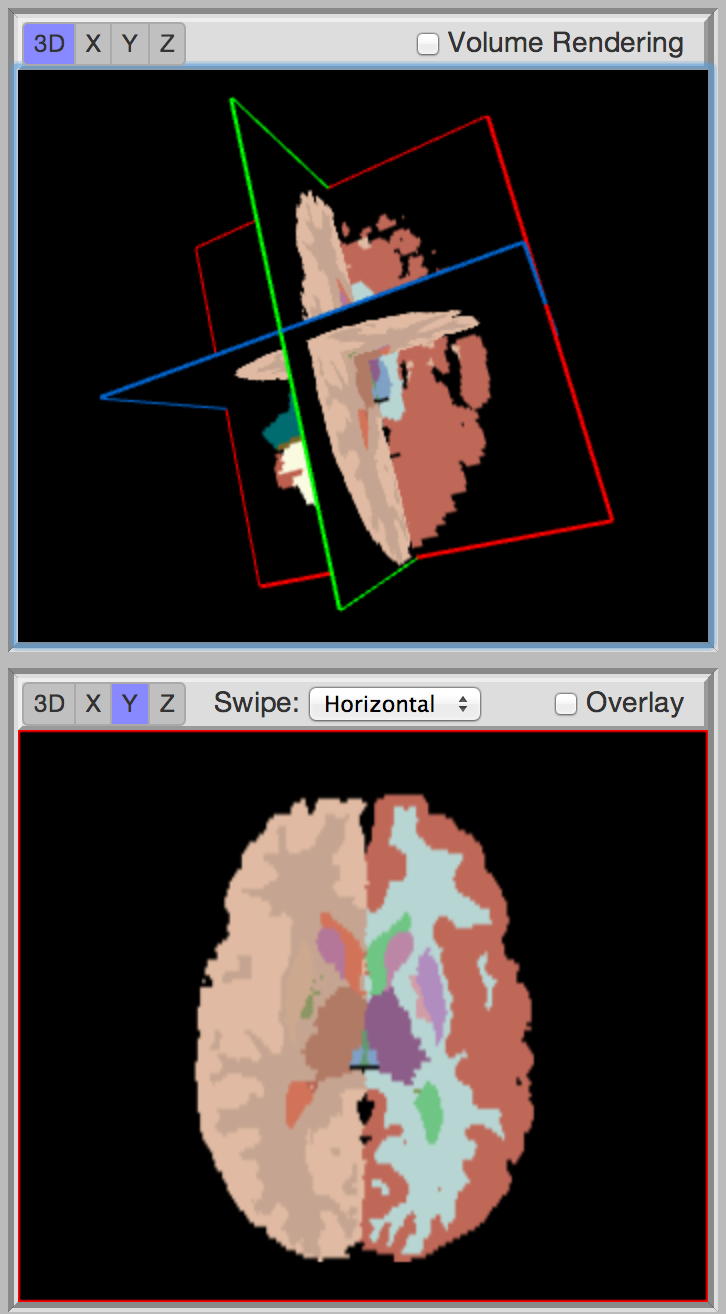
\includegraphics[width=52mm]{graphics/ColortableB_01.png}
  \caption{Colortable Option 'IDs'}
\end{subfigure}
\begin{subfigure}{.33\textwidth}
  \centering
  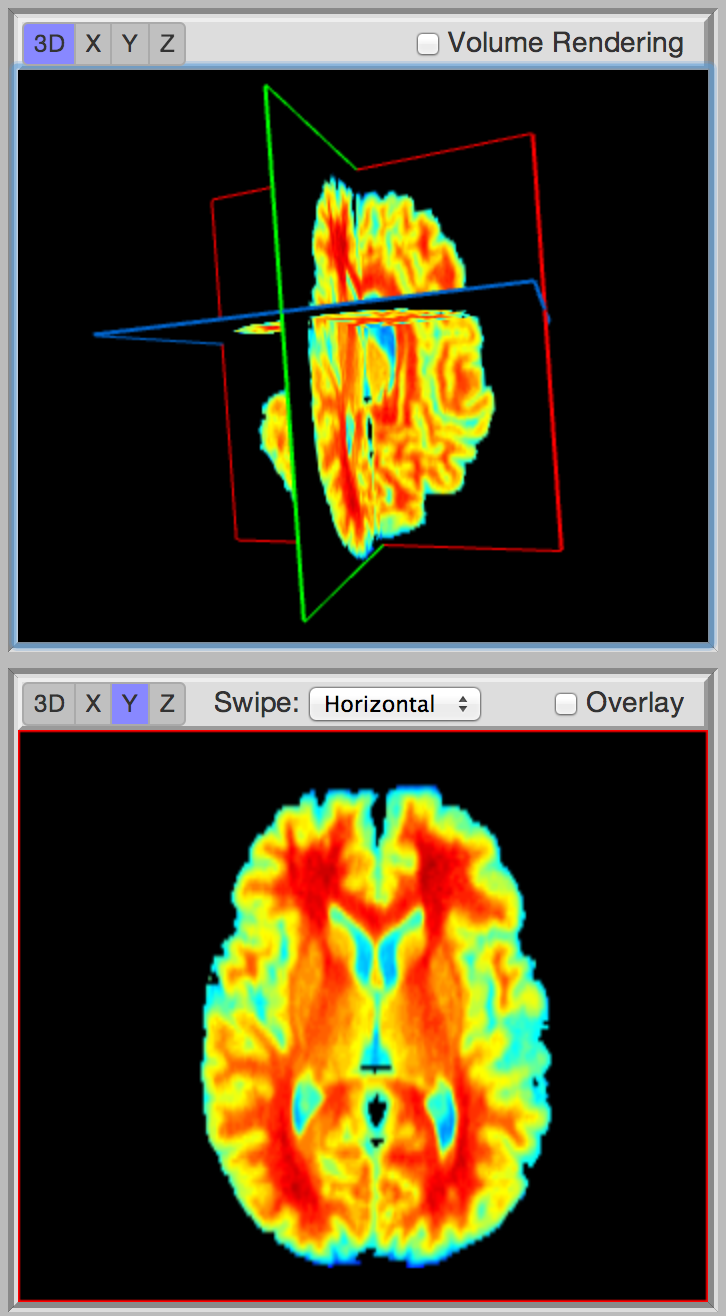
\includegraphics[width=52mm]{graphics/ColortableB_03.png}
  \caption{Colortable Option 'Heatmap'}
\end{subfigure}
\caption{Colortable Examples}

\end{figure}


Having finished this feature so far, it occured to me that I could actually speed the whole process up by having some hardcoded colortables in the code, and using them as a array to look up colorvalues when rendering the actual pixel. This was much easier to implement, loads much quicker as it is more efficient in only manipulating color at a pixel level rather then changing the color values of the whole volume. In the end I chose this method as I prefered the faster feedback. It has the limitation that the user can not load his own colortable, but this is a feature that could be added in future. For the moment, there are three colortables provided. Firstly, the standard colortable maps rgbs values directly to the same value. Secondly, an ID map maps values to different RGB values, which is intended for use with labelmaps. Thirdly, a type of Heatmap map has been included which maps the original RGB values from BLUE to RED to mimic the behaviour of a heat map. This was advised by the project supervisor, and an original heat mapping was supplied in a custom format, with only 64 integer mappings provided. I wrote a python script which would convert this into a\textit{JavaScript}array with 256 mappings. I also used a similar Python script to convert Slicer3D Wiki Colortables to useable\textit{JavaScript}arrays.



\subsubsection{Annotations}



The Annotations feature was addded in the last month and I was aware of time pressure. That is why initital design decisions had to be made to reduce wasted time later in the process. I decided on implementing rectangular annotations first, since that would make calculations easier to manage. Annotations would be\textit{JavaScript}objects with core members that were predefined (labelName, color, 3DPoints), and secondary attributes that would have to be computed on the fly (such as 2D Points for displaying on screen). Specifically, an annotation would be defined by 8 points in 3D Space. However to render it in a 2D View, 2D points had to be generated in screen space. I had intended the 2D points to be selectable in the Canvas View, so these 2D points should also be objects with custom attributes.

An initial UML diagram was desiged as below, although the final Annotation class contained quite a few more helper functions to help with the conversion from 3D to 2D space.

\begin{figure}[ht!]
\centering
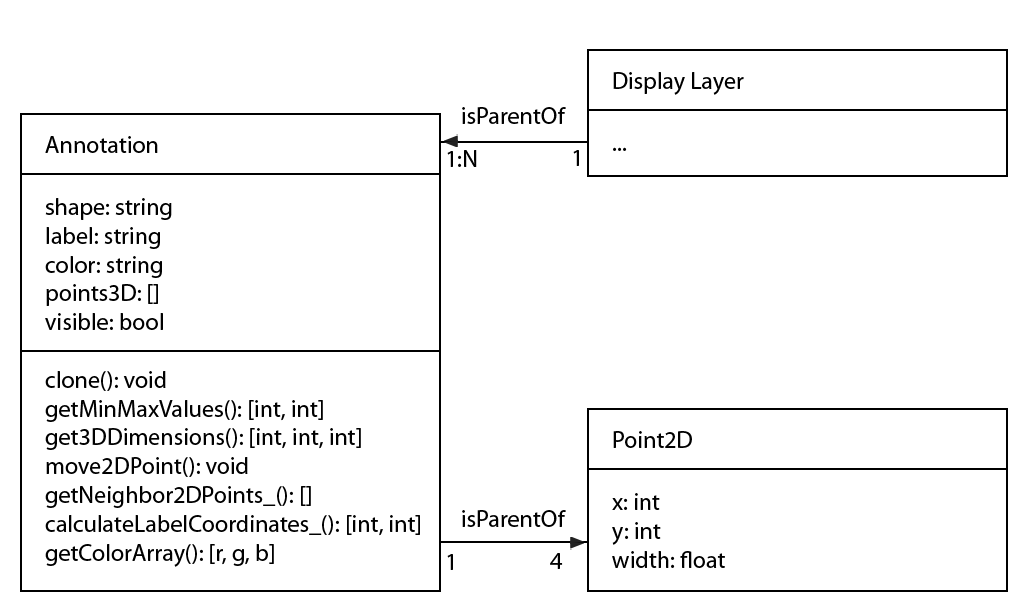
\includegraphics[width=140mm]{graphics/annoUML_01.png}
\caption{Annotation UML}
\label{fig:UIdesign1}
\end{figure}





The next step was to chose a data format and design the workflow. Initial tests were done with XML but to be somewhat cumbersome since some parsing is required and in the program the XML structures would have to be converted to\textit{JavaScript}objects. Therefore the much more intuitive JSON format was chosen, since this basically stores\textit{JavaScript}objects in readable form, and can be loaded directly into the program without almost any conversion required. The JSON format was originally derived from\textit{JavaScript}which explains its ease of use.

\begin{figure}[ht!]
\centering
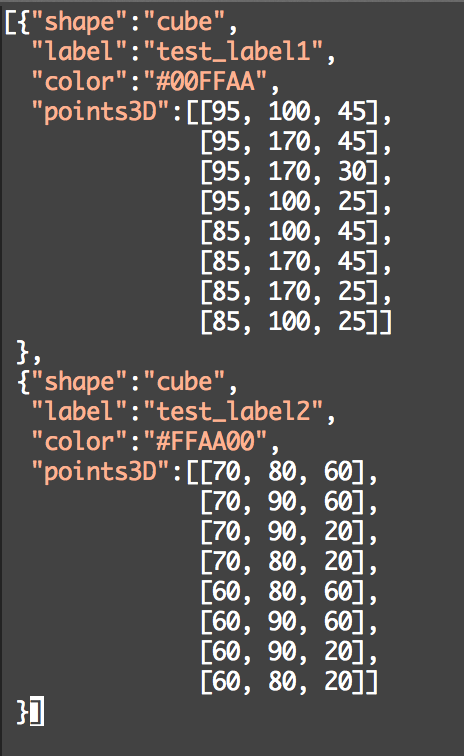
\includegraphics[width=80mm]{graphics/AnnoJSON_01.png}
\caption{Sample Annotations JSON file}
\label{fig:UIdesign1}
\end{figure}



Probably the most involved work was to figure out the conversion of 3D points to 2D screen space. The 2D points would be calculated by each XTK renderer separately, since the different views required different 2D screen space points. An array of the 2D points would be stored in the Annotation class. These points would then be updated whenever the position of the 3D points of the Annotation changed. The XTK renderer class has a function that translates 2D screen coordinates to 3D slice index coordinates which was a good starting point. I chose a simplified version of this function and implemented a conversion function, which appeared to work fine. I had to develop a much deeper understanding of the Volume File and its various Slice Depth Quantifiers, such as spacing and direction. These had to be integrated into the conversion since they define how the slices are spaced in relation to each other. A more detailed breakdown of these attributes will follow in the XTK subsection later in the Implementation section.


When I had finished my naive implementation, some small bugs were noticeable. For example all 2D points of an Annotation would sometimes jump by a pixel even when only one 2DPoint was being manipulated. I attributed this to some floating point or rounding errors, but could not track down where the errors were happening. Finally I had to admit that my simplified conversion function was not accurate enough, and I set out to reverse engineer the 2D to 3D conversion from the XTK library. This involved some inverse matrix multiplication, and in the end worked perfectly. These changes had to be made in the XTK renderer class.

In order for the user to manipulate the position of the Annotation points in screen space, I had to implement manipulatable corner points of the Annotation. This was made easy by the decision to have the 2D points. Initially I had contemplated creating a separate Manipulator class, but realised that this was superfluous and would just be repeating code. In the 2DPoint class I specified the position and width, so that in screen space I could make the 2DPoints appear wider for easier selection with the mouse. Some internal logic had to be added to the Annotation class, so that when the user changes the position of one 2DPoint, the neighboring points would also transform accordingly, since the shape had to always stay rectangular. I had to revise this is a couple of times, since in my first naive implementation, there would problems when the Annotation box would collapse so that all four 2D Points would be at the same screen space position. In the end I opted for limiting the size of the Annotation so that the points could never collapse to the same position.

\begin{figure}[ht!]
\centering
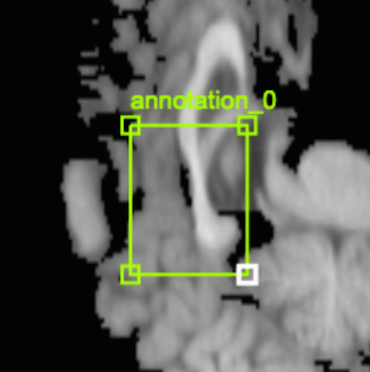
\includegraphics[width=60mm]{graphics/annoSelected_01.png}
\caption{Annotation with bottom right Point selected }
\label{fig:UIdesign1}
\end{figure}


An important part of the Annotation Management was the feature to download Annotations as a JSON file. However again due to Web Browser security restrictions, there is no 'Save File As' feature as I had imagined. However after some research, a viable alternative was found in that it is possible to 'download' a file (even if the code is running locally). This was deemed sufficient for this project, even if it does not allow for specifying the file name directly. With more time, it would be possible to add a pop-up window just like a 'Save as' dialog that would then trigger the file download.

Saving files to JSON format was straight forward due to the before-mentioned natural overlap of\textit{JavaScript}objects and JSON format. The saved files would only include the core information such labelName, color, 3D points and type.

To let the user specify a color for the Annotation, I needed to introduce a color picker. After some research, it became apparent that a host of color pickers were available online and it would be faster to use one of them than impement my own. I downloaded a couple of ColorPickers from the web, and deemed Blah's colorpicker to be better suited. It has a very basic interface that was deemed sufficient for chosing an Annotation color. Installing and implementing it into the project was also very straight forward.

Once I had implemented the code for creating and editing one Annotation, I created another layer system similar to main Display Layer management. Final tweaks to Annotation management include highlighting the Annotation Layer in the Layer View when hovering over or transforming one of the 2D Points.


\subsubsection{Labelmaps}

Adding Labelmaps proved to be relatively painless due to the time spent understanding the file loading process when implementing the colortables. The loader had to be forced to refresh when the labelmap was added on the fly. I restricted the program to only overlay one labelmap. I hooked up the opacity and colortables as for the Display Layers. I set the default colortable to chose the ID colortable preset, as that made more sense given the nature of labelmaps.

\begin{figure}[ht!]
\centering
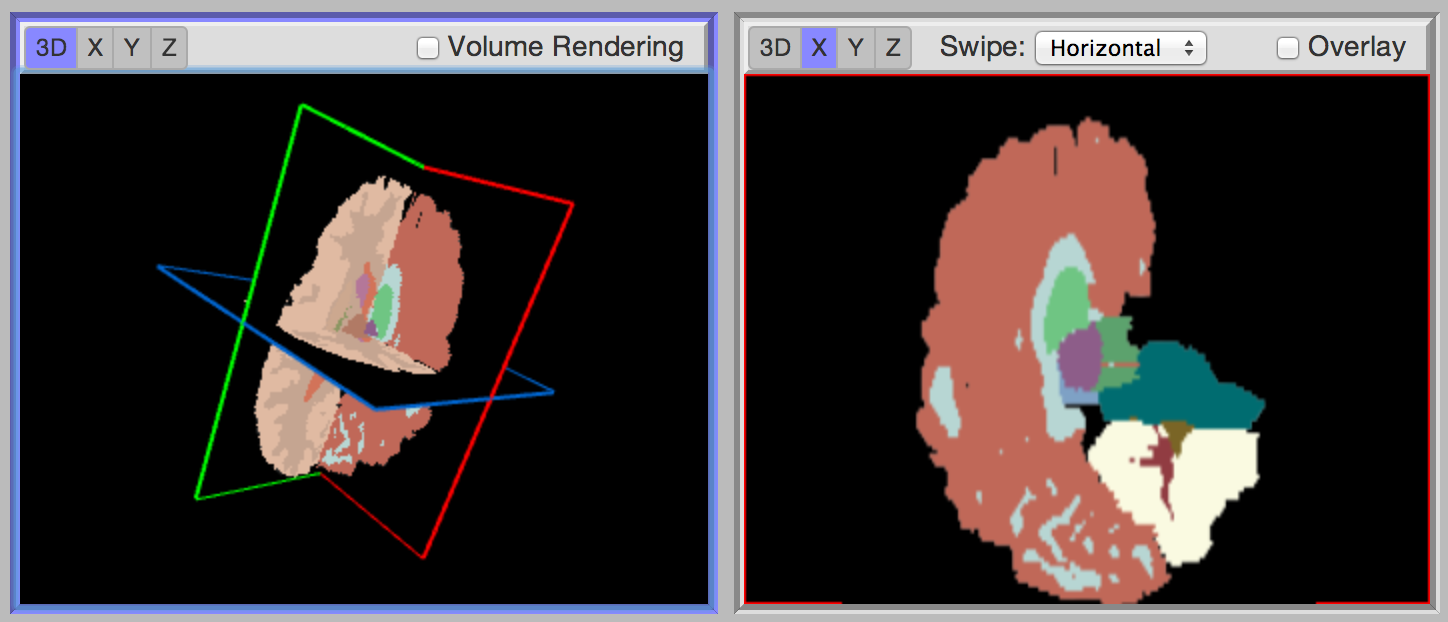
\includegraphics[width=170mm]{graphics/Labelmap_01.png}
\caption{Brain Scan with overlaid Labelmap}
\label{fig:UIdesign1}
\end{figure}



\subsubsection{Controls}

Dedicated effort was put into making the software intuitive for users to use, after having researched specific requirements for user input and understanding how many of these files could be inspected in a typical session. Since I was copying the pixels from the XTK render canvases into the custom Render Panels, I had to reinstate the controls that were already in XTK. However this also gave me some freedom to redesign certain controls.

I scrapped the mouse controls for brightness and contrast, since they were buggy, as discussed in previous sections, and there was not enough visual feedback for the user to see what was being changed. Instead I opted for traditional slider based methods, with numerical input fields on either side to clearly show which numbers were currently set. This works well in that it is very clear to the user how to manipulate the image, and it is more bug-free than the XTK implementation. Also the number input fields allow for precise control for the case that a user wants to recreate a certain brightness configuration.

All slice navigation and traversal was placed on mouse controls. The guidelines from the book helped inform the controls in that radiologist prefer to have as simple controls as possible since their work can consist of dealing with vast quantities of these kind of files, so any intricate control input method would soon get tiresome. Therefore the standard XTK input methods were kept mostly intact, so the middle clicking pans the camera, right-clicking zooms and left-click rotates in the 3D View. Since the left-click for the 2D Views was freed from controlling brightness, I assigned the traversal function to this, which allows the user to quickly reset all 3 slice indices. This was inspired by IMView (check!!) and prefered to XTK's default traversal input which requires the additional holding down of the 'Shift Key'.

Reinstating the mouse controls took some as I had to find out how to trigger the appropriate response in the XTK canvases. For 2D and 3D navigation, I had to study the XTK X.camera more closely. It turned out that I could access the X.camera's view matrix directly via an already implemented setter method, where indices 13 and 14 were synonymous with the X and Y position camera, and index 15 was the Z position. Therefore all I needed to do was calculate the relative movement to the currently selected HTML Canvas (by substituting the absolute mouse coordinates from the HTML Canvas coordinates), and convert this with an appropriate factor to X and Y numbers to be entered into the view matrix.
Likewise for zooming in the 2D Views, an adaptive zoom factor was implemented after discussion with the supervisor. The first normal implementation would zoom with a constant factor, but this would be more ineffective the further the camera was zoomed in on a slice. I implemented an adaptive zoom factor that interpolates between a linear zoom function to a square zoom function to counteract this effect.

To further add convenience for user input, I created a couple of keyboard shortcuts. To toggle between the A and B buffers, the user can press '1' or '2'. I was used to this from using the compositing software Nuke and have always found a frequently used short cut when comparing two images with each other, especially when looking for minute differences. This ties in with the idea that ScanView could be used to compare two medical image data files with each other. For the View Panels I also added the keyboard 'f' shortcut to recenter the camera after any panning, zooming or rotation had been applied, inspired by ITKSnap's image centering feature. This is achieved by storing the initial camera view matrix when the file is loaded, and loading this view upon key press. Adding these keyboard shortcuts is relatively trivial and more could and should be added, assuming that keyboard short cuts increase user speed. Some care had to be taken to ensure that the keyboard shortcuts do not get triggered when a text field is being edited.




\subsubsection{Error Handling}
An issue that is entirely related to the XTK library is how to let the user know that a certain file has not loaded. This was an important issue since a large variety of files downloaded from the Internet could not be opened with the XTK library. Various errors would be thrown in the loader.js and parser.js components of the XTK library, but there is no simple way to propogate this to the higher API-using layer, since the file loading is handled asynchronously and with event sending. There are no events implemented that signal the failing to load a file (other than failing to download a file via HTTP). Due to limited time, rather than adding these events into the XTK library, I added an error listener to the UI Layer which would call an errorHandler function whenever an error was thrown. This errorHandler function would then do a string comparison and cause a pop-up modal window to appear to inform the user of the specific error. This had the benefit of being able to screen for only certains types of errors.


\begin{figure}
\centering
\begin{subfigure}{.5\textwidth}
  \centering
  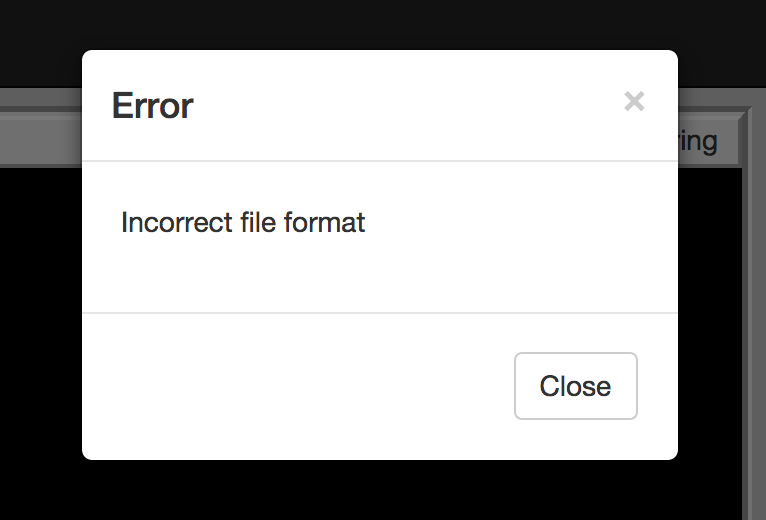
\includegraphics[width=82mm]{graphics/error_01.png}
  \caption{Error message for incorrect file format}
\end{subfigure}%
\begin{subfigure}{.5\textwidth}
  \centering
  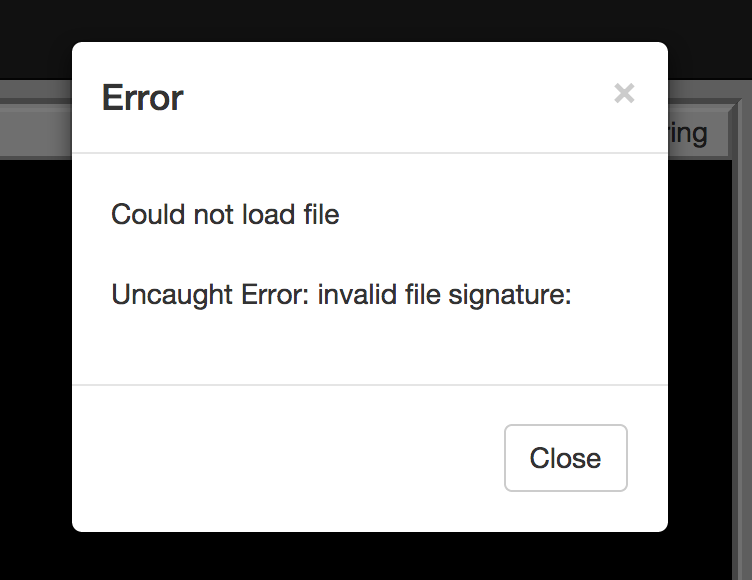
\includegraphics[width=82mm]{graphics/error_02.png}
  \caption{Error message for specific load error}
\end{subfigure}
\caption{Examples of Error Messages}

\end{figure}



\subsubsection{Slice Animation Feature}

This feature was added fairly late in the project, but it was relatively fast to implement. It had been suggested in the big medical book, and when talking to a radiologist, it seemed like it could be a useful feature which would relieve the user from manually having to scroll through a Volume file. I implemented this via a set of 5 buttons from the Twitter-Bootstrap library, commonly used to signal playing, stopping or rewinding a media file. I used the settimeout() method to recursively increment or decrement the current slice index (dependent on the viewer). At each recursion, it checks a guard variable whether to keep looping. The stop button changes this guard variable to on and therefore breaks the loop. I also trigger this break when the user uses the mouse scroll button, as I figured that the user might like to stop the animation easily other than by hitting the stop button. Almost by accident, it also provides the user to quickly navigate from to the minimum and maximum slice numbers for each direction by use of the fast-forward and fast-backward buttons.


\subsubsection{Polishing the User Interface}

Now with the program gaining shape, it was time to tweak the User Interface. This included the not very glamourous tasks of making sure that any Display or Annotation Layers would never be bigger than their container element by adding scroll bars. Luckily, this is a JQueryUI feature that is easy to implement, and one can specify along which axis one would like the scrollbars.

\begin{figure}[ht!]
\centering
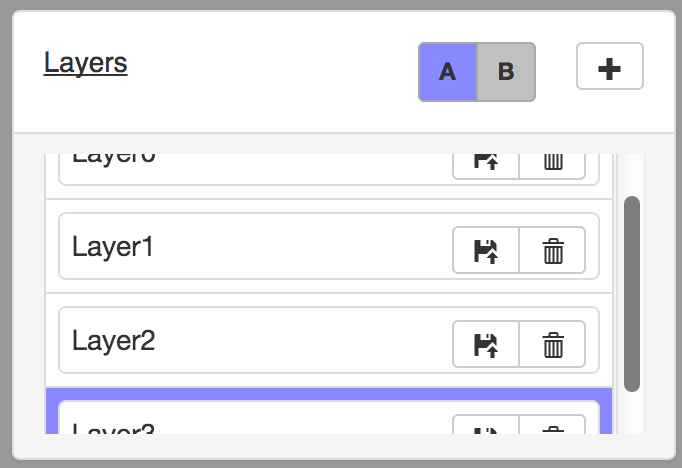
\includegraphics[width=90mm]{graphics/scrollbar_01.png}
\caption{Vertical Scrollbar for Display Layers}
\label{fig:UIdesign1}
\end{figure}

Furthermore, I implemented changes that would guide the user better in terms of using the software. This included disabling of all input and buttons in the Levels, Annotations and Labelmap tabs when no appropriate medical imaging file had been loaded yet. Also I added pop up windows were introduced to warn a user if the wrong kind of file was being loaded. Tooltips (from Twitter-Bootstrap library) were added to almost every button to help the user understand the intended functionality of each.


\begin{figure}[ht!]
\centering
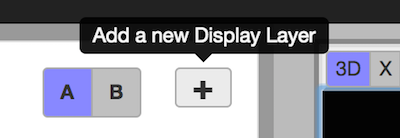
\includegraphics[width=70mm]{graphics/tooltipExample_01.png}
\caption{Twitter-Bootstrap tooltip example}
\label{fig:UIdesign1}
\end{figure}


\subsubsection{Deployment}


In order for users to be able to evaluate the product, some effort had to be put in to deploy the software to the web. I am hosting it on my personal webspace, which I prefered to hosting it on a local college server since I can send the site for feedback to people outside of Imperial College. I use FileZilla to upload the code, but wrote a Python script to facilitate the uploading, since manual replacing of files soon became tedious and time-wasting. The script will recursively copy each file of a specified directory to a designated space on my web space.

The deploying process went smoothly, as it had been desiged as a live webpage from the beginning. I added a page with some sample data for the user to download, tutorials resembling the protocols above together with screen capture videos. Furthermore an 'About' page was added which explained the main features of the program as well crediting various libraries and plug-ins that were used, as well as patch notes. 

Finally, an online survey by Survey Monkey was introduced to allow for convenient feedback by the user. Survey Monkey allows for free creation of surveys that are hosted online and accessible via a web link that can be sent by email or in this case embedded into a website. They also offer a host of analytical tools for investigating survey answers and data. The more advanced tools need to be paid for, but even the free tools allow for summary of results and inspection of individual responses. In lack of a proper beta test, this was deemed a quick way of getting feedback from different users. It was deemed important to ascertain whether the user has some experience with medical image data and viewing software, how much time the user spent with ScanView in order to estimate how thorough the usage was, which bugs were found and which features could be improved or added, The following questions were asked:

\begin{enumerate}
\item Have you worked with medical image data before? (Yes/No)
\item If yes, in what capacity have you worked with medical image data before?
\item Have you worked with medical image viewing software before? (Yes/No)
\item If yes, please states which programs you have used!
\item How much time did you spend with the ScanView program? (0 - 15 Minutes, 15 - 30 Minutes, 30 - 60 Minutes, 60 Minutes and more)
\item How convenient is the ScanView program to use? (Extremely convenient, Very convenient, Moderately convenient, Slightly convenient, Not at all convenient)
\item Do you think the ScanView program could be a viable alternative to comparable non-browser-based Medical Imaging Viewing software (eg. Slicer3D)? (Agree strongly, Agree somewhat, Not sure, Disagree somewhat, Disagree strongly)
\item Do you have any criticisms of the ScanView program?
\item What features would you like to see added to the ScanView program?
\end{enumerate}





A host of fixes have been uploaded since initial deployment, partially fixing outstanding bugs and implementing features requested from user feedback. More on this topic will be covered in the results section.





\subsection{Implementation Details/ Working with Libraries}

\subsubsection{Version Control}

To keep track of my project, I used Git. This was an obvious choice since it has been the DOC-prefered version control system as well as XTK being hosted on Github which I had to fork. I managed my own project code in a separate Version Control from my XTK fork in order to not confuse the two. Github proved as per usual very useful and reliable in tracking down changes from earlier versions as well keep submodules up to date for the XTK library. 


\subsubsection{Browser Developer Environment}

Initially I started developing in Chrome since it was my primary target for running the software. A few weeks my laptop broke due to accidental damage and I had to work in the labs, where I had problems running WebGL in Chrome, so I switched to Firefox. I soon found however, that Firefox leaves a lot to be desired for developing. The most important part of developing for me was the web console. With\textit{JavaScript}it is possible to print to this console, which I used endlessly. It also prints when a runtime error has occurred, complete with line number. This works great in Chrome, but in Firefox (on Ubuntu) at least, the line number would often be obscured. Any another problem is when printing a\textit{JavaScript}object to the console, it shows the final state of this object at the end of the code runtime. This means it is not possible to check the state of an object during runtime, only at the end. This caused some confusion until I had figured this out. Firefox is supposed to have a lot of plug-ins that can be downloaded, but in general I found Chrome to be much more convenient to use, and after a month managed to get a new laptop and returned to developing in Chrome.


\begin{figure}
\centering
\begin{subfigure}{.5\textwidth}
  \centering
  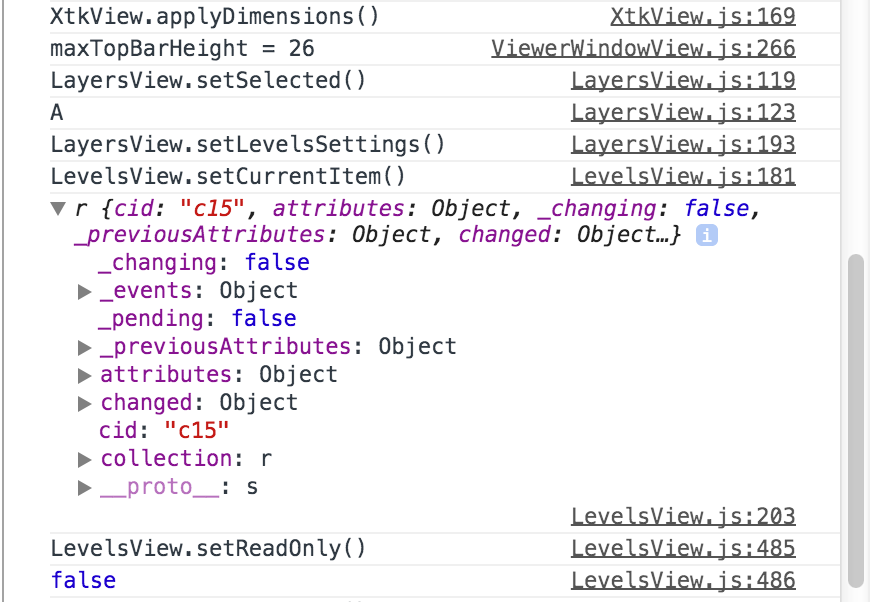
\includegraphics[width=82mm]{graphics/console_01.png}
  \caption{Chrome console showing\textit{JavaScript}Object}
\end{subfigure}%
\begin{subfigure}{.5\textwidth}
  \centering
  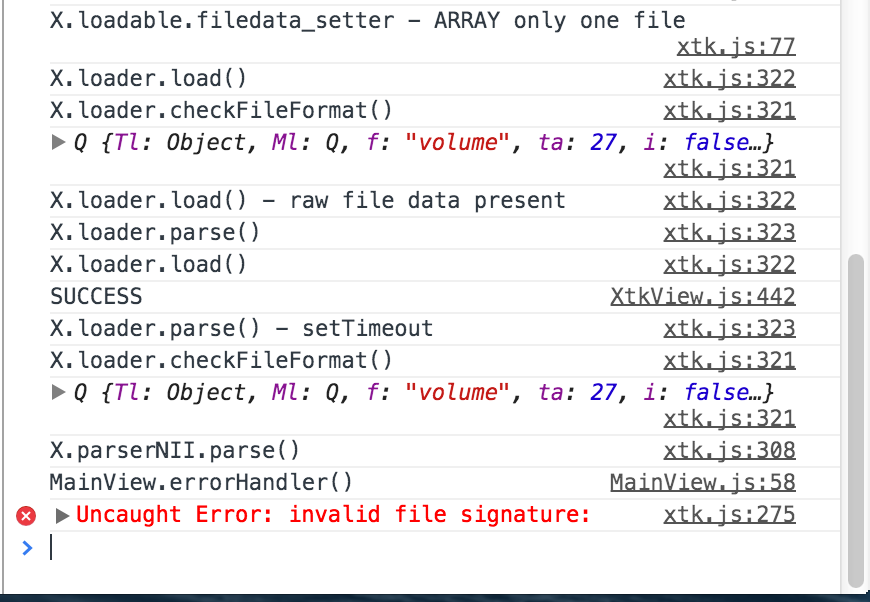
\includegraphics[width=82mm]{graphics/console_02.png}
  \caption{Chrome console showing error message}
\end{subfigure}
\caption{Examples of Chrome console displays}

\end{figure}

Chrome offers a variety of developer tools that come with the browser. First the 'Elements' tab provides the interactive HTML source code of the current web page. When hovering over a line of HTML, the appropriate element in website lights up. It also shows the current CSS rules that are being applied, with the option of toggling them on or off and getting a live preview. The 'Elements' tool is extremely helpful when debugging if the correct HTML correct has been written into the DOM or to check which CSS rules are currently active or have been overridden.


The next developer tool is the 'Network' tab. This shows the external libraries and source files are being loaded. It gives a good chronological break down of which library loaded when and how long it took. This proved useful in the beginning to see if the dependencies were handled correctly by RequireJS.

\begin{figure}[ht!]
\centering
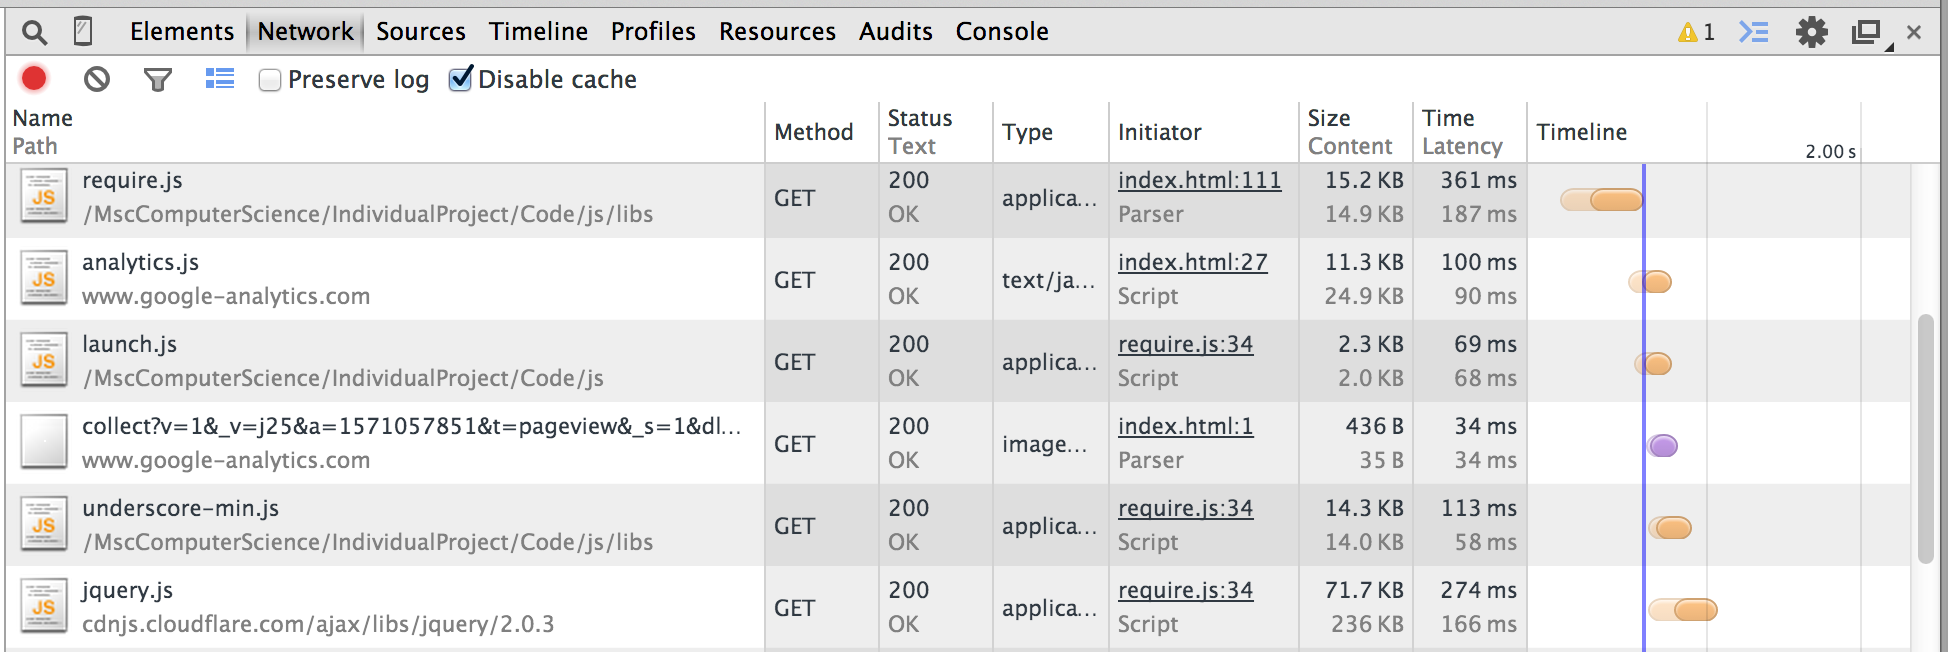
\includegraphics[width=140mm]{graphics/chromeNetwork_01.png}
\caption{Chrome Networks Tab}
\label{fig:UIdesign1}
\end{figure}


Chrome furthermore offers a debugger complete with break points, so it's possible to follow the flow of code  by individual lines or break points. This was used sparingly, as when working with XTK, the number of files that are being involved is huge and it would take too long to actually follow the code. Nonetheless it was helpful when I had to develop a deeper understand of the flow of control for example during when a file is loaded with XTK.

\begin{figure}[ht!]
\centering
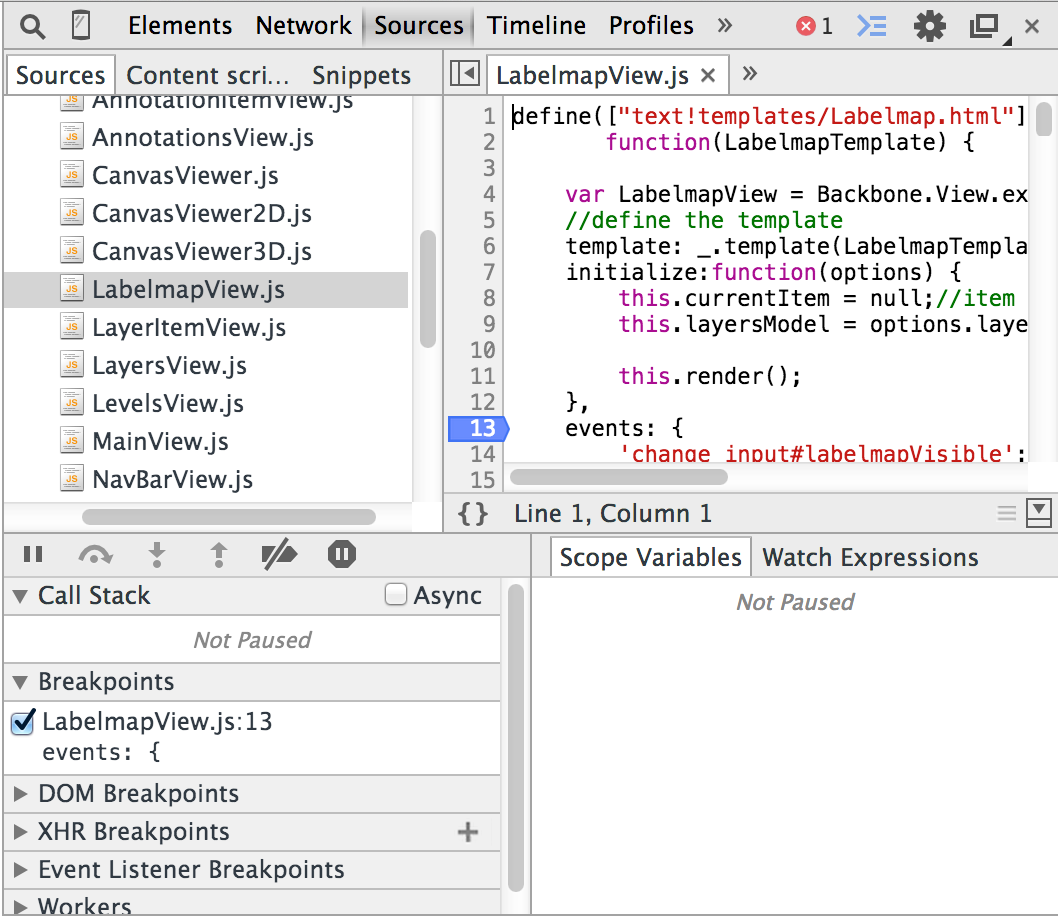
\includegraphics[width=140mm]{graphics/chromeDebugger_01.png}
\caption{Chrome Sources Debugger with one Breakpoint set}
\label{fig:UIdesign1}
\end{figure}



As there was some switching between Web Browsers, I noticed that Chrome and Firefox behaved differently sometimes. For example the layout would look drastically different in Firefox compared to Chrome, sometimes for reasons that were hard to track down due to large amount of variables in play. It appeared as if the css float command behaved differently, and place items to a different rule set. At other times, mouse navigation would not work in Firefox, since somehow mouse clicks where registered differently from Chrome. During the project, I spent time trying to bring up browser compatibility for both in parallel, but in retrospect I probably should have focused solely on Chrome, and then spent time making it work in Firefox and all other browsers, since they will also need custom work.


\subsubsection{JSFiddle}

Related to browser development, a tool I used a number of times was JSFiddle. This tool allows to on the fly testing of JavaScript, CSS and HTML. In fact, when asking for web developlement related questions on StackOverflow, answers are often posted with a working JSFiddle example. To create an example, one only needs to open JSFiddle and one can start coding. There are separate input windows for JavaScript, CSS and HTML code. It also features a windows that displays the resulting output. The link to this code can then be saved or sent to other people. All of the XTK tutorials are written as JSFiddle examples which allows for quick experimentation and testing of features. This was a really useful and convenient tool. 


\begin{figure}[ht!]
\centering
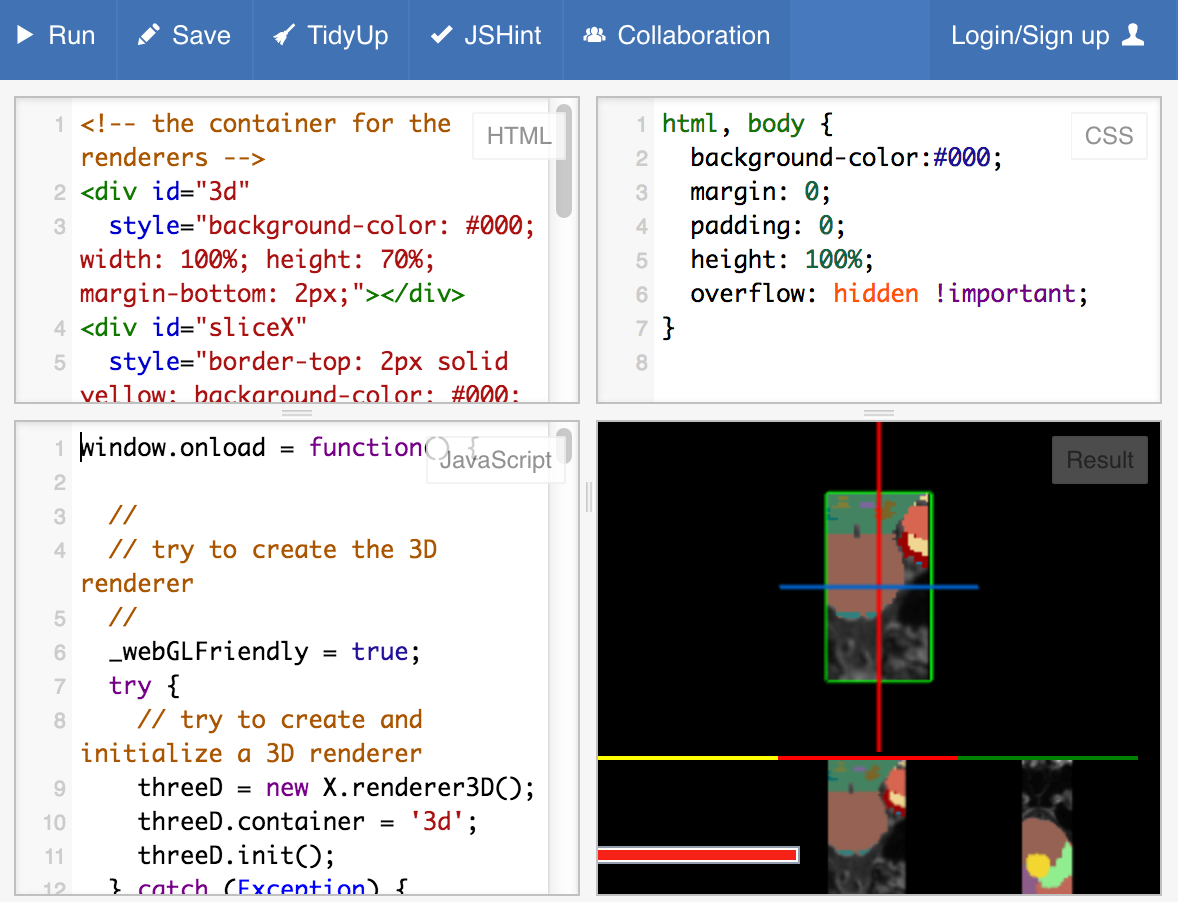
\includegraphics[width=140mm]{graphics/jsFiddle_01.png}
\caption{XTK Tutorial in JSFiddle Format}
\label{fig:UIdesign1}
\end{figure}




\subsubsection{XTK}


As already mentioned, the initial idea was to use XTK as an API to handle all the low level work to with loading and displaying Volume Files. As it soon became apparent, I had to dig deeper into the XTK library. Since XTK uses the goog closure library to minify the code, I first started to introduce print statements into the code in order to follow the flow better. However this became tedious quite fast and I figured out that is possible to run the uncompiled code with a few steps. This proved to be quite necessary since I was getting lots of errors at later stages of the project.





\begin{figure}[ht!]
\centering
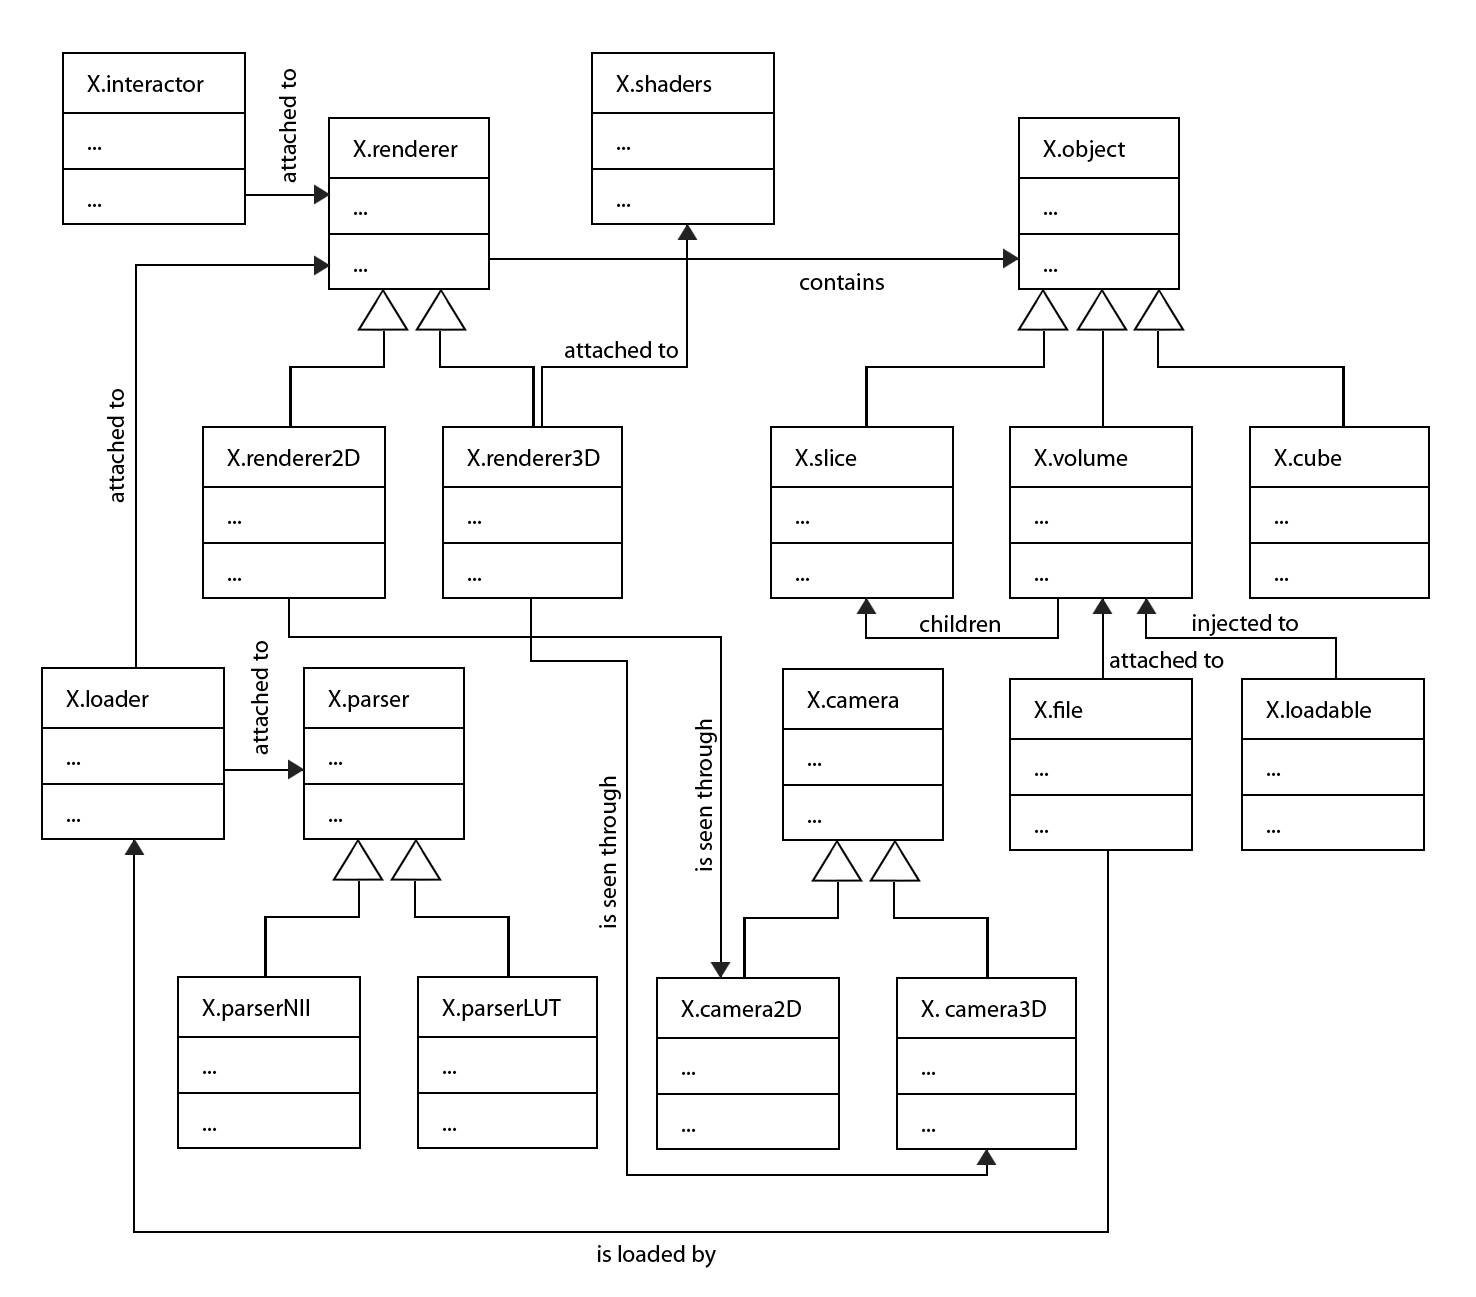
\includegraphics[width=170mm]{graphics/xtkUML_big_01.png}
\caption{Flow of Control of XTK renderer}
\label{fig:UIdesign1}
\end{figure}



When implementing the interactive loading of colorTables and labelMaps, I was forced to get a deeper understanding how the file loading process works. The Chrome debugger did help with this, and due to the complexity and the number of files involved, I had to draw diagrams which I would consult often. See below for the flow of control when loading a file.

\begin{figure}[ht!]
\centering
\includegraphics[width=140mm]{graphics/XtkFileLoad_01.png}
\caption{Flow of Control during XTK file load}
\label{fig:UIdesign1}
\end{figure}

In the example, a file is assigned to the volume. The volume is then added to the renderer (1) and the render() command is called (2). The render() call starts the continuous frame updating at 60 frames per second. At the same time, the renderer.add() function calls the internal update() function (3), which sets up event listeners for the volume. The overloaded update() function in renderer2D.js (4) gets the loader attached to the renderer, and calls the loader.load() function (5). The internal parse() function is called (6), which in turn determines the required parser (parserNII in this case) and calls its parse() function (7). At the same time, loader.parse() sets up an event listener to wait for a 'Modified' signal which will call the internal complete() function. ParserNII.js deals with the file format specific loading of data, and employs the reslice() (8) and reslice2() (9) functions to compute the current slice information of the volume. These are called three times - once for each orthographics view directions. Control is returned to parserNII.js after reslice2() has finished (10). Then an event signal is sent to loader.js, which triggers loader.complete() to be called (11). It also sets the volume's dirty flag to be true (which , among other uses, is used as a check by the renderer's render() function). The loader calls the modified() function in volume.js (12), which in turn calls its internal slicing\_() function (13), again once per orthographic view. In this last function, the current slice is set to be visible if it has been computed previously in the parser and parserNII. The slicing\_() function also gets called at other times, and if the current slice does not have any texture information loaded, the parser's reslice2() method is called from here for computation. Renderer2D's render() method which has been running continuously throughout this time, will recognise that the slice number has changed (from null to a specific integer number) and force a redraw of its pixels, thereby drawing the current slice texture to the screen. The render() function also checks if any dirty flags have been raised and will force a redraw accordingly.

If this process is being called for the first time, the modified volume will also send an Event Signal to the renderer that is has been added to, forcing the renderer.\_onShowtime() function to be called. This is useful in a setup with more than one renderer (such in ScanView's example where there exists one 3Drenderer and three 2Drenderers), as one can link the other renderers to start their render() functions when the loading has been done in the first renderer. Personally I do not actually like this method, since it forces an interdependence on the viewers and I would have prefered a more modular approach. When asking about this StackOverflow, one of the XTK developers agreed that the current solution is not ideal.





For renderer2D.js, when the user changes the index of one of the slide directions, the update function is called and the new slice texture calculated. This slice texture is then stored in a local buffer in the volume object, called children so as not to have to recalculate this slice when the user returns to this index at a later point. The renderer.js object itself is running at a specified frame rate, and will update if it detects that one of a number of things has changed in the volume. Slice index changing is one of them. It was this that caused some problems when causing a redraw after reapplying a colortable or a labelmap. All the current checks would not cause a redraw, since I had not changed the slice index, but rather data that was affecting the current slices. So I had to find another way of triggering this redraw. In the end I opted for querying for the X.slice's sliceId attribute, which is a unique identifier number that gets changed every time a slice is recomputed. This way I could finally register the update. 




Xtk deals with its 2D and 3D renderers quite differently. One difference is in how the update function works. For renderer3D.js the update function becomes a recursive call with 60 plus iterations depending on the loaded volume.


I needed to write various setters and getters for attributes that I need to get access to, which was trivial to implement. Adding some functions required for inverting ijk to xy values proved to be more challenging and took much longer.

I tried to follow the style guide which is posted online in using camelCase typing with underscores at the appropriate places for attributes and functions.

There seem to be some issues and bugs with XTK. One of these is that some files do not load properly, so more advanced file handling should be added. Also the mouse controls for threshold and window setting work in a way that is not intuitive and not reversible, so that after left-clicking and dragging a few times, the image will not return to its original brightness anymore. This could be because there are two attributes (min and low) to set for both threshold and windowing.




\subsubsection{RequireJS}

RequireJS proved invaluable for determining correct dependencies for loading\textit{JavaScript}libraries.
As I am using more than a handful of libraries which are also dependent on one another, I needed the ability to ensure that they had loaded correctly. The issue is that the modules are loaded asynchronously, so a module that depends on a another module could easily load before the other (as opposed to in sequence loading from function programming). A good exampe for this is the tooltips that I implemented towards the final stages of the project. Both jQueryUI and twitter-bootstrap provide tooltips. In both cases they are initiated by the same function call, however they look quite distinctly different. I wanted to use the twitter-bootstrap tooltips as they seem more aesthetically pleasing. Without determining the load order with RequireJS, whenever I reloaded the software a different tooltip style would pop up, depending on which library loaded first. This kind of race condition is of course undesirable.

Another example is of course XTK itself which relies on JQuery and UnderscoreJS. RequireJS really was a life saver for these situations. The screen shot below shows the ordered nature of loaded modules, using Chrome's Network tab. Without RequireJS, the loads would happen a lot more randomly.


\begin{figure}[ht!]
\centering
\includegraphics[width=120mm]{graphics/requireOrder_01.png}
\caption{Ordered module loading with RequireJS}
\label{fig:UIdesign1}
\end{figure}





\subsubsection{Backbone}

Working with Backbone worked well after a steep learning curve in the beginning, especially because I had to set it up in parallel with RequireJS (discussed in the next subsection).

I sometimes was unsure of whether to follow the event-based design or normal functionl design. It is tempting to communicate between components via events, but I found it also makes it a lot more difficult to debug, since it's not easily visible which pieces of code are listening to an event that is fired.

Similarily, I started out using Backbone's collections which are a type of array for models. However this seemed not necessary and I just converted to use an array of Display Layers instead.

Issue with DRY between models and views. It is tempting to put functionality into the views, rather than the models.

//CHANGE THIS AROUND, ADD TO HISTORY... of annotations

One issue came up with arrays and the 'change' event. When changing the contents of an array, the 'change' event does not get fired. This is because the base address of the array does not change. In order to work around this, I had to clone the arrays everytime I wanted to change their contents. I ended up packaging this sort of behaviour in classes that had arrays as members. This issue came up predominately with Annotations, since Annotation objects are stored in a array structure in the Display Layer Model. Also Annotation objects contain arrays of 3D and 2D points.






\subsubsection{JQueryUI}

Generally speaking, for any HTML page element, both the look and the functionality have to be considered, as implementing them can be quite complex. This is why a lot of libraries have been created that provide generalised elements such as buttons, file loaders and more complex UI elements. A few like JQueryUI and Twitter-Bootstrap have been become very popular and have been used in this project. They have the benefit of providing both the CSS style definitions as well as predefined\textit{JavaScript}functionality for the elements. 

Some features from this library were utilised, such as the tab functionality for the 'Levels', 'Annotations' and 'Labelmaps' tabs. Also, the sliders for setting Brightness, Threshold and Opacity were taken from this library, as they provided a convenient solution both for the design and for the functionality.


\subsubsection{Twitter-Bootstrap}

This library was used to style the webpage consistently and to make use of their icons, buttons and tooltip functionality.

The library provides a host of useful icons and button presets, such as button groups which were used when grouping buttons close together like the 'Load' and 'Delete' button for each Display Layer. This added a more sophisticated look to the software without the need for individual styling of buttons by writing custom CSS classes.

Adding the tooltips proved more involved than initially thought. For dynamically added HTML elements such as the Display Layers, custom tooltip options would have to be used and set in order to make them work correctly. So instead of having a general purpose solution, custom settings had to be set for each tooltip. Also, since Twitter-Bootstrap and JqueryUI both provide tooltips that called by the same initialisation function, sometimes errors would appear in the browser console, stating that a conflict had been caused. Fortunatly, JQueryUI allows for downloading a custom build where the tooltip feature has been disabled.

Furthermore, creating modal warning screens when the user attempts to load a file with the wrong extension was made very easy with Twitter-Bootraps modal screen. Again, styling this manually and creating the logic behind it would have been very time consuming.

Twitter-Bootstrap supplies a host of interactive UI elements such as buttons, tooltips, pop up windows, tabs, navigation bars, progress bars and more. It is a widely used library - in June 2014 it was the No.1 project on GitHub with 69,000+ stars and 25,000+ forks (Wiki).


\begin{figure}[ht!]
\centering
\includegraphics[width=100mm]{graphics/twitterBootstrap_01.png}
\caption{Examples of Twitter-Bootstrap components used. Panel (left), Modal (top right) and Button Group (bottom right)}
\label{fig:UIdesign1}
\end{figure}



All things considered, this libary proved to be very useful and saved a lot of time.




\subsubsection{Google Analytics}

Google Analytics is a tool by Google that provides detailed information of website usage. I installed it to get a clear picture of how many people would be using the website. I have used Google Analytics in the past and have been impressed by the comprehensive overview it provides. It shows the number of unique and returning visitors, average session duration, feedback on which browsers and operating systems they were using, which city and country it was viewed from. Additionally for mobile devices it even shows the screen resolution.

Implementation is very easy by just copying an HTML script code snippet and pasting it into any website that the user would like to track the usage for.

\begin{figure}[ht!]
\centering
\includegraphics[width=160mm]{graphics/googleAnalytics_01.png}
\caption{Google Analytics Website Usage Statistics}
\label{fig:UIdesign1}
\end{figure}








\newpage


\section{Results and Evaluation}

In order to evaluate the software, two components were chosen. The first was to test one of the main claims of this project, namely that the website runs on a variety of computer setups, thereby freeing the user of having to use a specific desktop tool for a specific platform. Secondly, the software has been deployed on the Internet and has been sent to a number of users for evaluation via a survey. Finally the software will be evaluated against the aims set forth at the beginning of the project.
Evaluation of main client?







\subsection{Review of Features}

\subsubsection{Comparing to initially set requirements}

When comparing the final features of ScanView with the list of initial requirements, it appears that all of the primary requirements have been implemented successfully.


Regarding secondary requirements, only a few have been implemented. This is mainly due to lack of time and complexity of some of these requirements. In retrospect it is much more clear that some secondary requirements are harder to implement than others. For example adding Measuring Tools would be quite easy, since a lot of the basic functionality that would be required is in place, such as conversion from screen space to volume space. Sharing data online would be much more demanding to implement, since it would require dealing with network and could be subject to entire other project (even though an implementation via DropBox would be feasible).



\begin{center}

  \begin{tabular}{| l | l |}
    \hline
    Primary Requirement & Implemented \\ \hline \hline
	Loading NII file & Yes\\ \hline
	Viewing file in 2D and 3D & Yes\\ \hline
	Navigation in 2D and 3D & Yes\\ \hline
	Brightness and Contrast controls & Yes \\ \hline
	Loading NII Labelmaps & Yes \\ \hline
	Loading additional NII files for comparison & Yes \\ \hline
	Different color-lookups provided & Yes \\ \hline
	Sample Data Provided & Yes \\ \hline

  \end{tabular}\\
\end{center}

\begin{center}

  \begin{tabular}{| l | l |}
    \hline
    Secondary Requirement & Implemented \\ \hline \hline
	Paint Custom Labelmaps & No\\ \hline
	Save Labelmaps to computer & No \\ \hline
	Create and save Annotations & Yes \\ \hline
	Method of sharing data & No \\ \hline
	Image filters & No \\ \hline
	Measuring Tools & No \\ \hline
	View volume file as 3D model & Yes \\ \hline
	Animation along axis & Yes \\ \hline



  \end{tabular}\\
\end{center}









\subsubsection{Comparing with other Web Browser based programs}

In terms of the final feature list, ScanView distinguishes itself from the currently available web-based Medical Image Programs. As most online programs are very basic, ScanView's features outnumber them. 

The software that it resembles most closely is SliceDrop, also in part due to its common heritage. ScanView improves on SliceDrop in a number of ways. ScanView is more dynamic in that it allows interactive file loading and deletion similar to a standard desktop software program. It allows to load several Volume Files (via Display Layers) which can be compared visually due to the implemented Buffer System. Furthermore file load errors are handled more completely by letting the user know the error message via a message pop-up. In SliceDrop, file load errors are only printed to the developer console, which the standard user can not be expected to check. Both ScanView and SliceDrop enable volumetric rendering, since this is a common feature of the XTK library. ScanView's View Panels are more free to display custom information via the Overlay toggle. In terms of navigation, both feature the same set transformations. ScanView adds the convenience feature of resetting the view camera to the start position of the camera. SliceDrop does not feature an Annotation System like ScanView does. SliceDrop does allow for custom loading of color tables, whereas ScanView's final implementation relies on predefined colortables. SliceDrop also allows for downloading .nii files of currently viewed data, which ScanView is not able to do. Both programs can overlay labelmaps on top of Volume Files. Although not implemented, there is code in SliceDrop's code base that would enable loading and saving to DropBox. So while both programs have different feature sets, ScanView is better at comparing multiple files and adding annotations. Furthermore it provides a more interactive feel with its Display Layer Management system and adjustable Layouts.




Compared Papaya and DICOM Web Viewer, ScanView's feature list looks even more favorable. Both programs are very light-weight, feature only 2D Views and no multiple file loading. NEED MORE TEXT HERE.




\begin{center}

  \begin{tabular}{ | l | l | l | l | l |}
    \hline
    Feature & ScanView & SliceDrop & DICOM Web Viewer & Papaya \\ \hline \hline

Loading NII file & Yes & Yes & Yes & Yes\\ \hline
Loading Other file formats & No & Yes & ? & ?\\ \hline
Loading multiple files in one session & Yes & No & No & No \\ \hline
Error handling for loading files & Yes & No & No & No\\ \hline
Orthogonal Views & Yes & Yes & Yes & Yes\\ \hline
3D Perspective View & Yes & No & Yes & Yes \\ \hline
Volumetric rendering & Yes & Yes & No & No\\ \hline
Volumetric and 2D rendering overlaid & No & Yes & No & No \\ \hline
Comparing several files to each other & Yes & No & No & No\\ \hline
Annotations & Yes & No & No & No\\ \hline
Loading of custom colortables & No & Yes & No & No \\ \hline
Loading predefined colortables & Yes & No & No & No\\ \hline
Saving of Data & No & Yes & No & No\\ \hline
Online File Sharing & No & No* & No & No\\ \hline
Adjustable Layouts & Yes & No & No & No \\ \hline
Segmentation Tools & No & No & No & No \\ \hline

  \end{tabular}\\



*Not currently available but being worked on


\end{center}



\subsubsection{Comparing with Desktop-based programs}

Naturally due to the limited time frame of this project, ScanView can not compete in terms of feature richness with other available programs. Given the time, it should however be possible to reach a similar level of feature completeness. Technically, it seems feasible. Actually, ScanView does aim to match in terms of features...


\begin{center}

  \begin{tabular}{ | l | l | l | l | l |}
    \hline
    Feature & ScanView & 3DSlicer & ImView & ITKSnap \\ \hline \hline

Loading NII file & Yes & Yes & Yes & Yes\\ \hline
Loading Other file formats & No & Yes & ? & ?\\ \hline
Loading multiple files in one session & Yes & No & No & No \\ \hline
Error handling for loading files & Yes & No & No & No\\ \hline
Volumetric rendering & Yes & Yes & No & No\\ \hline
Volumetric and 2D rendering overlaid & No & Yes & No & No \\ \hline
Comparing several files to each other & Yes & No & No & No\\ \hline
Annotations & Yes & No & No & No\\ \hline
Loading of custom colortables & No & Yes & No & No \\ \hline
Loading predefined colortables & Yes & No & No & No\\ \hline
Saving of Data & No & Yes & No & No\\ \hline
Online File Sharing & No & No* & No & No\\ \hline
Adjustable Layouts & Yes & Yes & No & No \\ \hline
Segmentation Tools No & Yes & No & Yes \\ \hline

  \end{tabular}\\


\end{center}


\subsection{Reviewing of Use Cases}

Considering the use cases that were stated at the beginning of this report:

\begin{itemize}

\item A user loads two medical images files ... for image comparison and compositing.

\item A user wants to create a custom label map by highlighting a certain section of a loaded scan...

\item The user wants to create annotations for a file... (and) can save out this files as a custom data file.

\item A user wants to communicate with another user who is not present in the same location...
\end{itemize}

the first and the third have been implemented in this project. The comparison of two medical image files is possible by loading them into two separate Display Layers and Buffers, and then setting the opacity slider and switching or swiping between the Buffers. Secondly, the Annotations feature covers the third use case by enabling the user to create custom Annotations, edit, label, color and to save them out in JSON format. As was pointed out by the project supervisor, this could be used for example for annotating a large set of volume files for a specific feature or organ. This data set could then be used to by machine learning algorithms for automatic detection of similar graphical features.

The second and fourth use case have unfortunately not been implemented, but as they both fell into the secondary requirement category, this is not surprising. Implementing the primary requirements simply took too much time. However at least the case of creating custom label maps is quite within reach with maybe a month of more development time, since it some of the basic methods such as 2D screen to 3D volume (and vice versa) point conversion methods are already implemented.




\subsection{Protocol Testing across different platforms}

In order to judge whether the software fulfils its purpose of running on a variety of operating systems and Web Browsers, a number of protocols were tested across a range of computer setups. It was tested on the four most commonly used Web Browsers and on Windows, OSX Mavericks, Linux (Ubuntu) and Android. Additionally a test was run for the Apple I-Pad. The protocols were designed to mimic what a typcial user would do with the software as well as to get a comprehensive coverage of all the features.


\subsubsection{Protocols}

\subsubsection*{Protocol 1 - Basic Viewing of Volume File }

- Create a Display Layer\\
- Load a medical image data file (.nii)\\
- Test navigation - pan/zoom/rotate/traverse\\
- Test window levels\\
- Test threshold\\
- Test changing color lookup\\
- Test the different layouts\\
- Test switching Camera Views

\subsubsection*{Protocol 2 - Creation of Annotation }

- Create a Display Layer\\
- Load a medical image data file (.nii)\\
- Create a new annotation\\
- Change annotation label\\
- Change annotation color\\
- Change annotation vertex points

\subsubsection*{Protocol 3 - Loading and Saving of Annotations }

- Create Display Layer\\
- Load a medical image data file (.nii)\\
- Load/Import annotation JSON file\\
- Change annotation color\\
- Change annotation vertex points\\
- Save out annotation


\subsubsection*{Protocol 4 - Labelmaps }

- Create Display Layer\\
- Load a medical image data file (.nii)\\
- Load a labelmap file\\
- Set opacity of labelmap file\\
- Change color lookup for labelmap

\subsubsection*{Protocol 5 - Display Layer Management }

- Create Display Layer\\
- Load a medical image data file (.nii)\\
- Create a second Display Layer\\
- Load a second medical image data file (.nii)\\
- Toggle between buffers\\
- Test opacity slider\\
- Test horizontal swipe\\
- Delete First Display Layer\\
- Test basic viewing\\
- Delete Second Display Layer




\subsubsection{Testing Environments}


\subsubsection*{OSX Mavericks}

For OSX the website was tested on the latest OSX Mavericks Operating System, installed on a Mac Book Pro. All protocols were run successfully for both Chrome and Firefox.\\

\noindent Hardware:\\
- Model Name:	MacBook Pro\\
- Processor Name:	Intel Core i7\\
- Processor Speed:	2.3 GHz\\
- Number of Processors:	1\\
- Total Number of Cores:	4\\
- L2 Cache (per Core):	256 KB\\
- L3 Cache:	6 MB\\
- Memory:	16 GB\\


\noindent Operating System:\\
- OS X 10.9.4\\

\noindent Browsers Tested:\\
- Chrome Version 36.0.1985.143\\
- Firefox Version 31.0\\
- Internet Explorer - Not available
- Safari Version 7.0.6 (9537.78.2)\\

\subsubsection*{Windows 7}

For Windows the website was tested on Windows 7, running on a virtual machine on a Mac Book Pro with the same specification as the previous section.\\

\noindent Hardware:\\
- Running via VMware Fusion on same MacBook Pro as used for testing OSX Mavericks\\

\noindent Operating System:\\
- Windows 7 Professional N Service Pack 1\\

\noindent Browsers Tested:\\
- Chrome Version 36.0.1985.143\\
- Firefox Version 31.0\\
- Internet Explorer 8.0.7601.17514\\
- Safari Version 5.1.7\\


\subsubsection*{Linux Ubuntu}

For Windows the website was tested on Windows 7, running on a virtual machine on a Mac Book Pro with the same specification as the previous section.\\

\noindent Hardware:\\
- Running via VMware Fusion on MacBook Pro as used for testing OSX Mavericks and Windows 7\\

\noindent Operating System:\\
- Ubuntu 14.04 LTS\\

\noindent Browsers Tested:\\
- Chrome Version 36.0.1985.143\\
- Firefox Version 28.0\\
- Internet Explorer - Not available\\
- Safari Version - Not available


\subsubsection*{IOS}

For IOS the website was tested on a Ipad Air. It was fairly clear that this would not work well, since IOS is a closed system that does not allow a free file structure as required by this software. However it was still checked to get a wider coverage of platforms.\\

\noindent Hardware:\\
- Ipad Air\\

\noindent Operating System:\\
- IOS V.XX\\

\noindent Browsers Tested:\\
- Safari Version XX



\subsubsection{Protocol Results}

\subsubsection*{OSX Mavericks}

All protocols were run successfully for both Chrome and Firefox. When using Safari, they were issues with loading Annotations and Navigation control. This should be fixable by simply investing more time into the project.\\


\begin{center}
  \begin{tabular}{ | l || l | l | l | l |}
    \hline
    Protocol & Chrome & Firefox & Internet Explorer & Safari \\ \hline \hline
    1 & Yes & Yes  & - & No   \\ \hline
    2 & Yes & Yes & - & No \\ \hline
    3 & Yes & Yes & - & No  \\ \hline
    4 & Yes & Yes & - & No  \\ \hline
    5 & Yes & Yes & - & No  \\
    \hline
  \end{tabular}
\end{center}

\subsubsection*{Windows 7}

All protocols were run successfully for Chrome. The file loading failed for Firefox and therefore all subsequent tests failed as well. However when testing on a machine in Imperial College, ScanView did work perfectly on FIrefox, so more tests will have to be performed to analyse the source of this discrepancy. There were lots of issues with Internet Explorer, which was expected since it is renowned for being difficult to code for and not following conventions of the other browers. Safari was not tested on Windows 7, since a stable version could not be installed.

\begin{center}

  \begin{tabular}{ | l || l | l | l | l |}
    \hline
    Protocol & Chrome & Firefox & Internet Explorer & Safari \\ \hline \hline
    1 & Yes & No  & No  & - \\ \hline
    2 & Yes & No & No & - \\ \hline
    3 & Yes & No & No & - \\ \hline
    4 & Yes & No & No & - \\ \hline
    5 & Yes & No & No & - \\
    \hline
  \end{tabular}

\end{center}

\subsubsection*{Linux Ubuntu}

On Ubuntu, both Chrome and Firefox performed well. Chrome worked perfectly as intended. With Firefox, some layout issues were notices, for example that the Labelmap Tab was beneath the Annotation tab and not next to it. Safari and Internet Explorer were unfortunately not available for testing.

\begin{center}

  \begin{tabular}{ | l || l | l | l | l |}
    \hline
    Protocol & Chrome & Firefox & Internet Explorer & Safari \\ \hline \hline
    1 & Yes & Yes  & -  & - \\ \hline
    2 & Yes & Yes & - & - \\ \hline
    3 & Yes & Yes & - & - \\ \hline
    4 & Yes & Yes & - & - \\ \hline
    5 & Yes & Yes & - & - \\
    \hline
  \end{tabular}

\end{center}


\subsubsection*{IOS}

As expected, most functionality did not work on the Ipad. The display layer management worked fine, however the user is not able to load a file, since the default file opening only allows opening photos. However, it would be possible to circumvent this by implementing a solution that uses a file loading app, such as Dropbox. The Driopbox API seems to allow for this, so it could be possible given extra time.

\begin{center}

  \begin{tabular}{ | l || l | l | l | l |}
    \hline
    Protocol & Chrome & Firefox & Internet Explorer & Safari \\ \hline \hline
    1 & - & -  & -  & No \\ \hline
    2 & - & - & - & No \\ \hline
    3 & - & - & - & No \\ \hline
    4 & - & - & - & No \\ \hline
    5 & - & - & - & No \\
    \hline
  \end{tabular}

\end{center}

Looking at the results from all browser tests, ScanView seems to be stable for Chrome on all three platforms. This is encouraging, since most time was spent developing for this platform. Firefox support comes in second place, as it works fine on both OSX and Ubuntu, but not on some Windows 7 computers. For Internet Explorer and Safari, ScanView fails to supply even basic functionality of file loading, and more time would have to be spent getting it working for these two browsers.


\subsection{CPU performance}

It has to be noted that the CPU usage is higher in ScanView than the original XTK apps. This is large part due to the design choice of copying the renders from the XTK renderers as discussed in the implementation. This accounts for the majority of the computational overhead. CPU comparisons were run in the Chrome - OSX environment and look as follows.
In order to improve performance, RequestAnimationFrame was used. Need some more text explaing what this does.



\subsection{Usage and User Feedback}

\subsubsection{Google Analytics}

At the time of writing, the following results were collected from Google Analytics about the usage of the website.

\begin{figure}[ht!]
\centering
\includegraphics[width=160mm]{graphics/resultsAnalytics_01.png}
\caption{Google Analytics Website Usage Statistics as of September 2nd, 2014}
\label{fig:UIdesign1}
\end{figure}

The website has had 32 unique visitors over the 13 days since going live on August 21, 2014. The average session time was 5 minutes and 30 seconds. The majority of users viewed ScanView with Chrome (74.6\%), the recommended browser, on OSX (61.9\%). Ideally the 
website would be online for a longer time to get a more complete picture in terms of usage. 

\subsubsection{Survey Responses and Feedback}

Unfortunately only three people answered the survey, but I received two more individual responses with reviews and suggestions by email.
For the survey, 2 of the 3 users had used medical imaging software before (such as ITKSnap). The users spent 0 to 30 minutes with the website. For convenience, the responses were 'extremely convenient', 'very convenient' and 'moderately convenient', which suggests that convenience was judged to be better than average. When asked if the software could be an alternative to desktop software, the answers were 'agree somewhat', 'disagree somewhat' and 'not sure' which is undecisive, and in retrospect deservedly so, as most desktop software reviewed had a lot more features and development time compared to ScanView. In terms of criticism, the following were raised (combined with individual email responses):

\begin{itemize}
\item High CPU usage on Ubuntu laptop (with Chrome)
\item Loading stack of images rather than isotropic volume does not work
\item Volume rendering not working with Sample Data
\item Cannot delete Labelmaps
\item Lack of Undo functionality
\item Lack of clarity in terms of which orthographical view is which, should be labeled more clearly
\item Issue with Opacity and 3D-Views
\item Cursor changes to test selection mode during View Panel interaction
\item No 3D Views for any Display Layer after second Display Layer
\end{itemize}


The following additions or changes were suggested from survey and email responses.

\begin{itemize}
\item Add support for .nii.gz files (has been added since)
\item Add support for other file formats
\item Combine "Create Display Layer" and "Open File" actions, as they are implied to go together (has been added since)
\item More info could be displayed about the specific files
\item Be able to apply colortable selectively to Canvas Views
\item Export and save out datasets (in different formats)
\item Add a play feature for the 3D view that would rotate a camera around the volume data
\end{itemize}

 
As mentioned, it would have been beneficial to run a more comprehensive beta test to get more user feedback for ScanView, which unfortunately was not possible in the time of this project (as development took up so much time). Five responses does not quite provide enough data to get a sense of how ScanView is perceived by users in general. It would probably help to incentivise survey participation somehow, in order to get more responses. However the answers I did get were very helpful and useful in pointing out deficiencies. I managed to add some fixes to the few criticisms that I received. File loading error handling is much more robuts now, with enabled nii.gz support. Some spelling mistakes have also been fixed, as well as some name changes made in order to be less confusing. It is frustrating to receive bug reports of errors that I am not able to reproduce, and could therefore have to do with the specific hardware of the user. At this point it shows that an anonymous survey is not ideal to tackle this kind of problem, and a direct dialogue with users would be preferable. Alternatively to the survey, I could have added a more detailed bug report page, where the user could have specified their browser, version and hardware. Ideally this could be detected automatically like Google Analytics already does to a degree.


\subsubsection{Outstanding Feedback}

I sent a link to the software to the XTK developers in order to get their feedback, but at this point in time have not heard back from them. Also two radiologists in London and India have been contacted through private channels, but their feedback is also outstanding at this point.





\section{Conclusions}

In terms of the initial purpose of this project to investigate whether it is possible to create a feature rich medical image viewer which works in a Web Browser, the course of the project seems to suggest that it is indeed possible given current Web standards with HTML5 Canvas Element and the WebGL standard becoming common-place. The XTK library forms a solid base for adding more features such as in this project. In order to add more complexity, a method was chosen which requires more CPU power than the normal XTK library.

In terms of creating a functioning piece of software, more time would have been benificial to iron out bugs. Also it would have been great to have a bigger pool of sample data to work from, as there seem to certain files that do not open with this software. Given the limited time frame and man power, ScanView does not match the feature richness and performance of high-end software solutions. However this is not a limitation based on the technical possibilities of Web Browser technology, so should be feasible. One issue might be the complexity of scale, as software solutions such as BrainSomething are 400MB. That would be too much to load in a Web Browser, so a more complex memory management would be required.

The experience of this project suggests that with a team of dedicated programmers and proper funding, a viable web-browser based medical imaging tool could be created that could rival current desktop based applications in terms of features richness, performance and user experience.



\newpage
\section{Future Work}


\subsection{Limitations and Bugs}

At the time of writing, there are a number of known bugs and issues to resolve:

\begin{itemize}

\item Annotations are not positioned properly with specific files
\item Not all .nii files open, due to issue with XTK library
\item ColorPicker pop-up for Annotations will open too low in screen if too many Annotation Layers have been created, so that the 'OK' button can not be pressed
\item Number input fields for Window and Threshold are too small with bigger numbers
\item When panning, object in Viewer Panel does not follow mouse cursor 100\%
\item High CPU usage has been reported on Linux Ubuntu and Chrome. This is due to a general architecture decision and would take considerable time to redesign
item When loading more complex data sets, the responsiveness drops noticeably

\end{itemize}


\subsection{Future Improvements}

As has has been shown, using a library like XTK can be used successfully to write a cross-browser web app for inspecting medical image data. In terms of expanding the software, a number of features could be added which could make the application more useful and user-friendly.

\begin{itemize}
\item Add support for other file formats other than .nii
\item Re-enableing the loading of custom color tables
\item DropBox support could be built into the software to enable file loading, saving and sharing. Additionally this could enable the tool to be used on IOS.
\item More work to style the website for different resolution screens.
\item Paint tools could be implemented as has been done successfully by BrainBook, to paint custom Labelmap
\item Support for 4D data sets could be implemented. This would have be done at a low level in the XTK library, but should conceptually not be too hard since it would just be a series of volumes. Appropriate and meaningful user interface additions could be made without much difficulty.
\item Smart sliders should be added, so that for Levels and Threshold, the bar can be dragged instead of having to manipulate for ends.
\item Interactive splitters could be introduced so that the user has more freedom in defining the size of individual View Panels
\end{itemize}


In this specific case, I would probably chose to rework the XTK library more closely to add the features that I have added with ScanView, however at a lower level. There exists a performance trade-off based on the decision to have custom Render Canvases copying image data from the XTK canvases. This was done to add extra functionality more easily, but it adds computational requirements. It should be possible to add this high level functionality into the XTK library itself.










\newpage

\begin{thebibliography}{1}


http://www.statista.com/statistics/263401/global-apple-iphone-sales-since-3rd-quarter-2007/

http://webdesignfromscratch.com/html-css/how-html-css-js-work-together/

http://en.wikipedia.org/wiki/Model%E2%80%93view%E2%80%93controller#mediaviewer/File:MVC-Process.svg

\end{thebibliography}

\newpage

\section{Appendix}



- Talk about DRY, UML Style Diagrams!




\end{document}
